\chapter{仿真结果}
\label{chap:model2}

\fontsize{12bp}{14.4pt}

\section{锁模的条件}
\subsection{调制深度}
以$FSR = 25GHz$,泵浦功率$P_{in} = 100mW$,改变调制深度进行仿真。\\
随着调制深度的增加,系统的稳态经历了混沌,周期性振荡,双脉冲,单脉冲振荡,单脉冲五个阶段。
\begin{figure}[htbp]
    \centering
    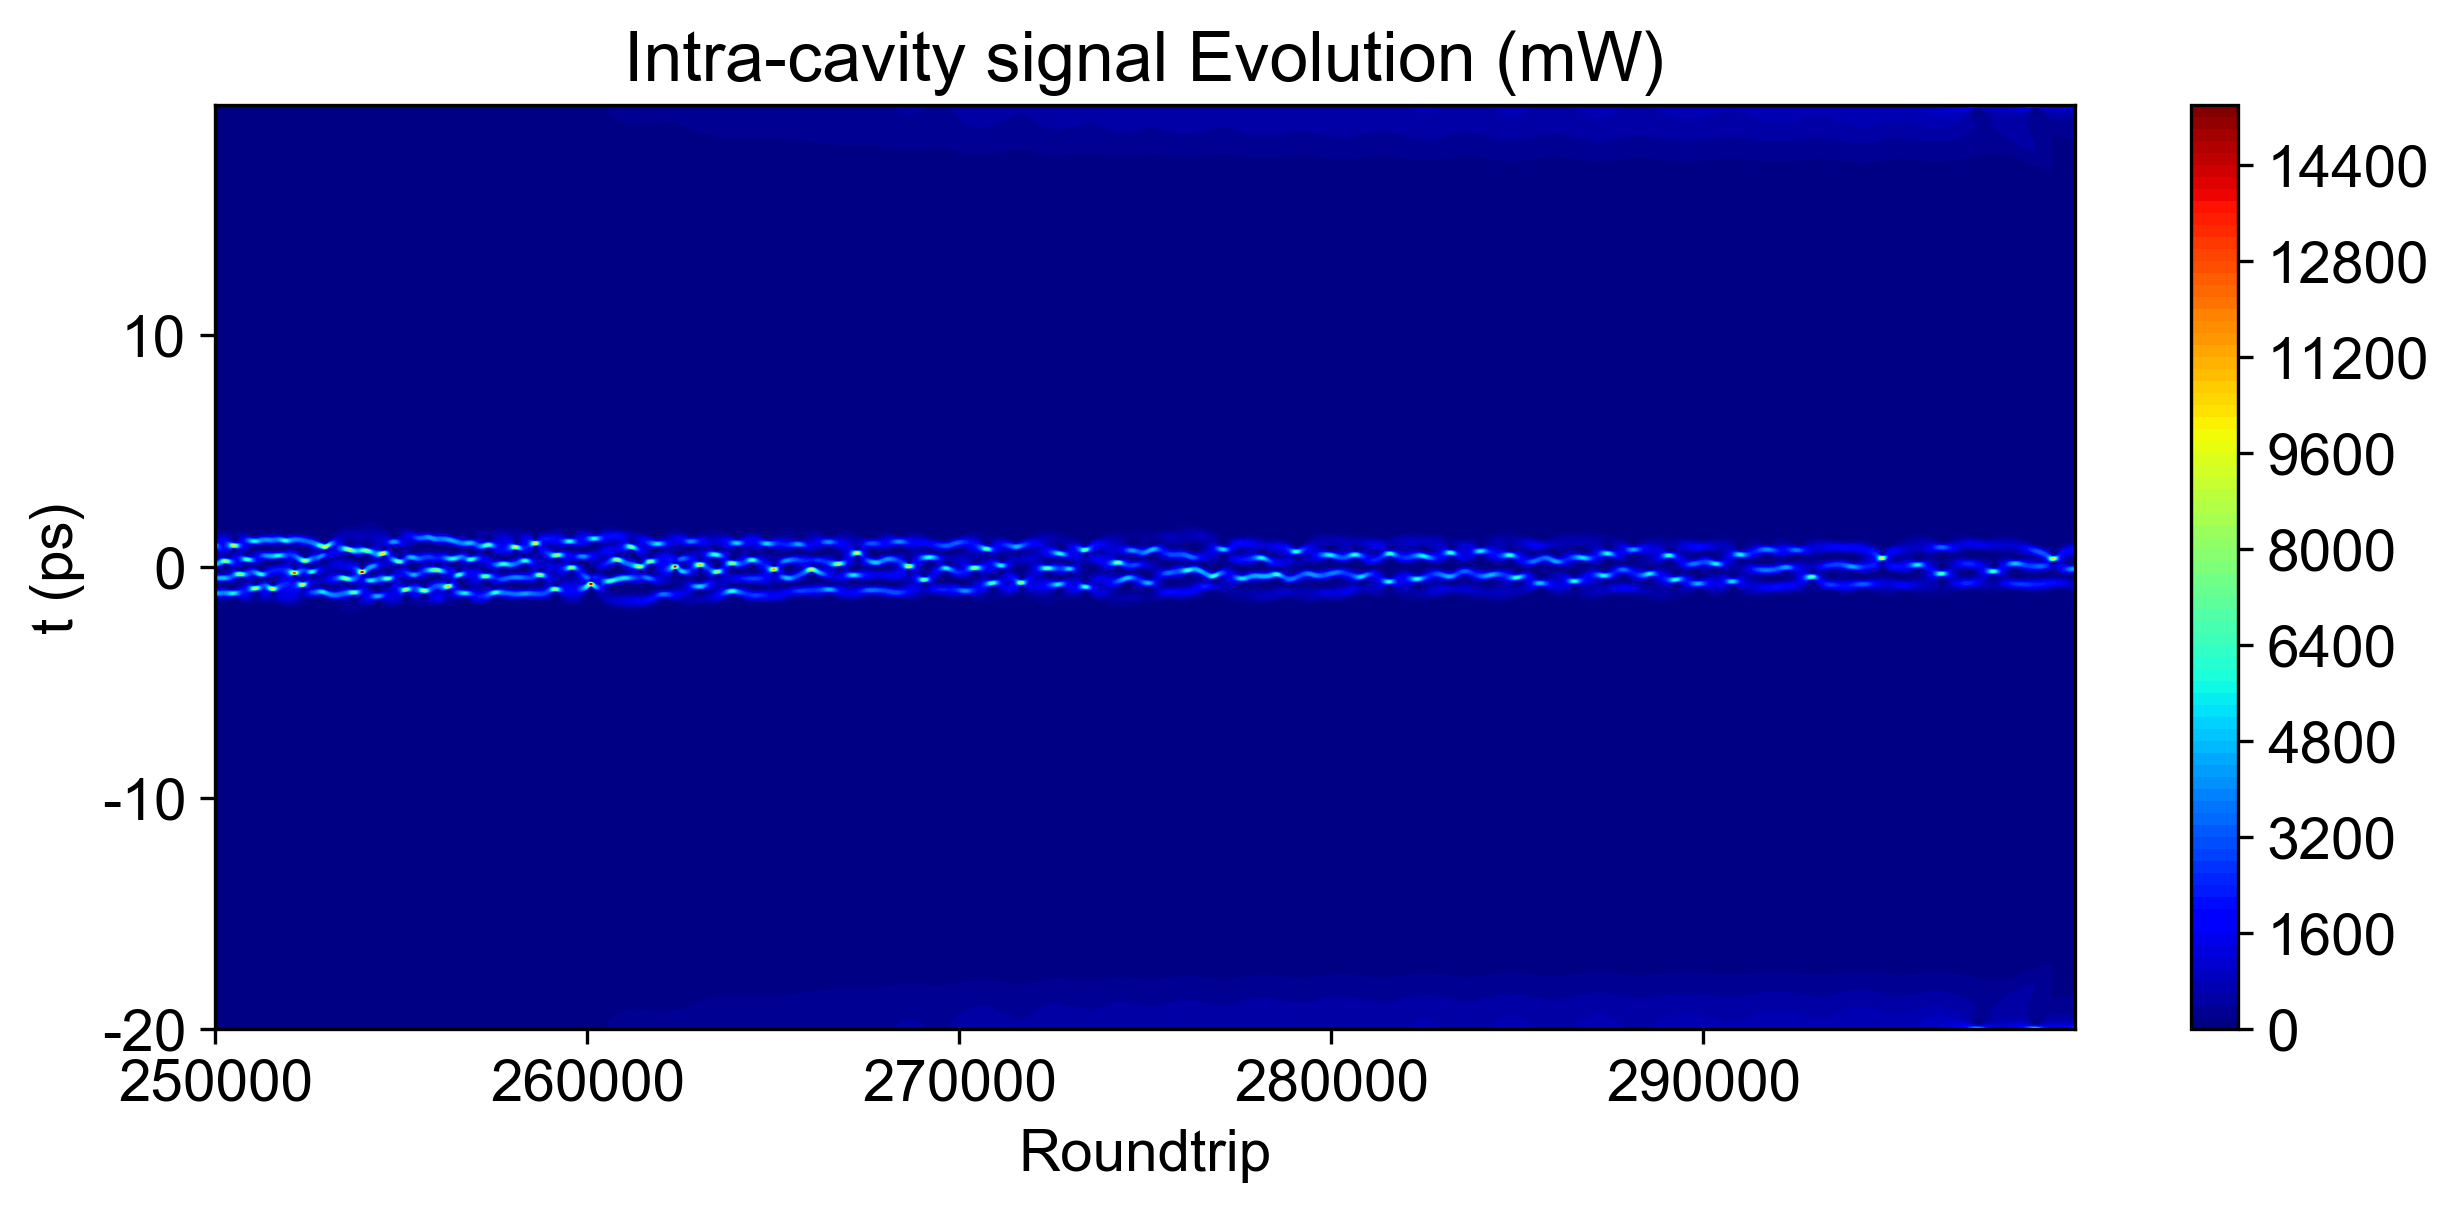
\includegraphics[width=0.48\linewidth]{figure/fig_12.png}
    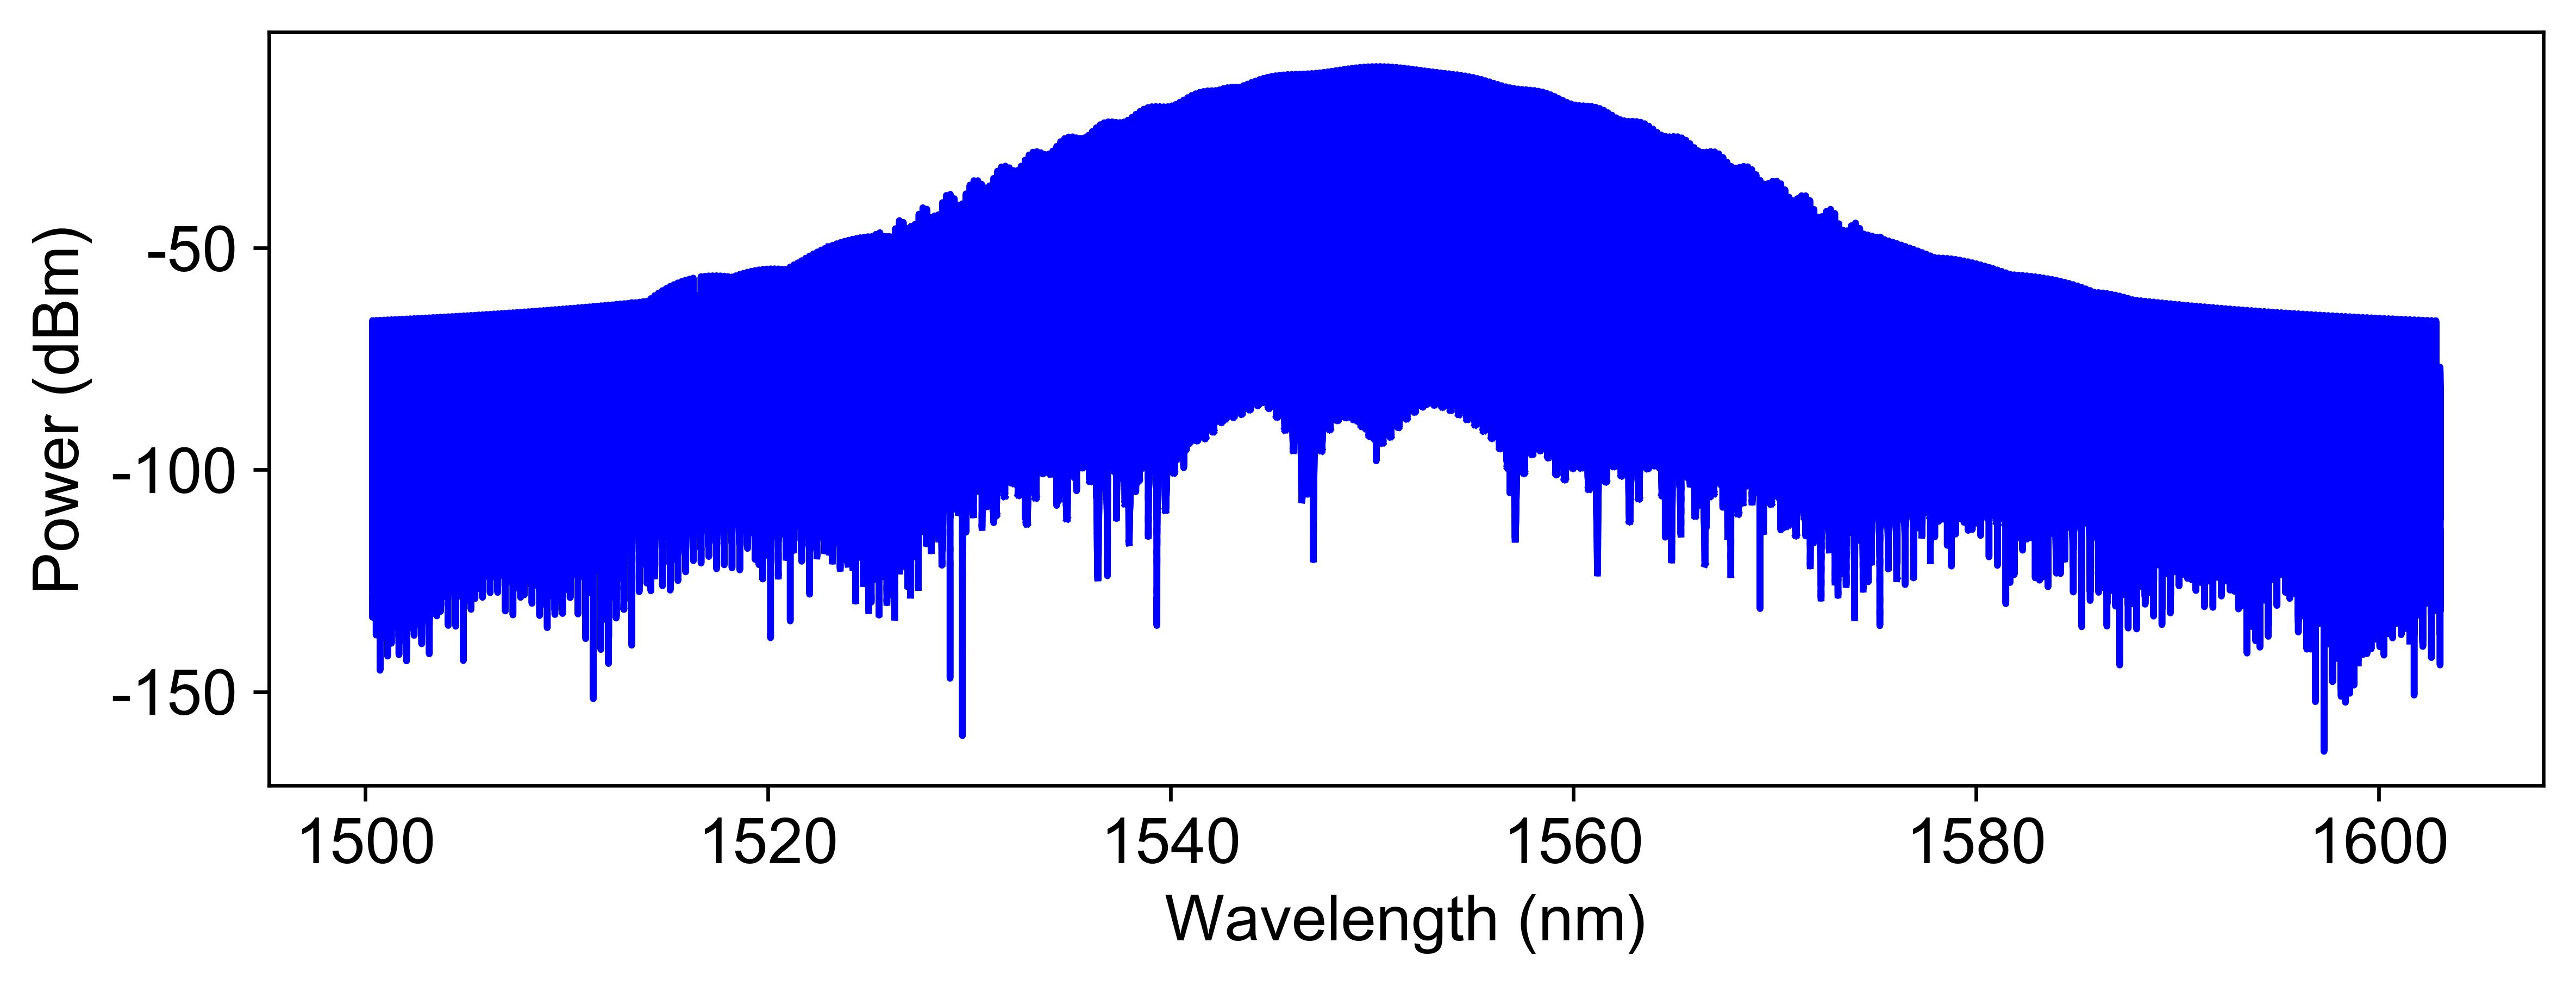
\includegraphics[width=0.48\linewidth]{figure/fig_12_0.png}
    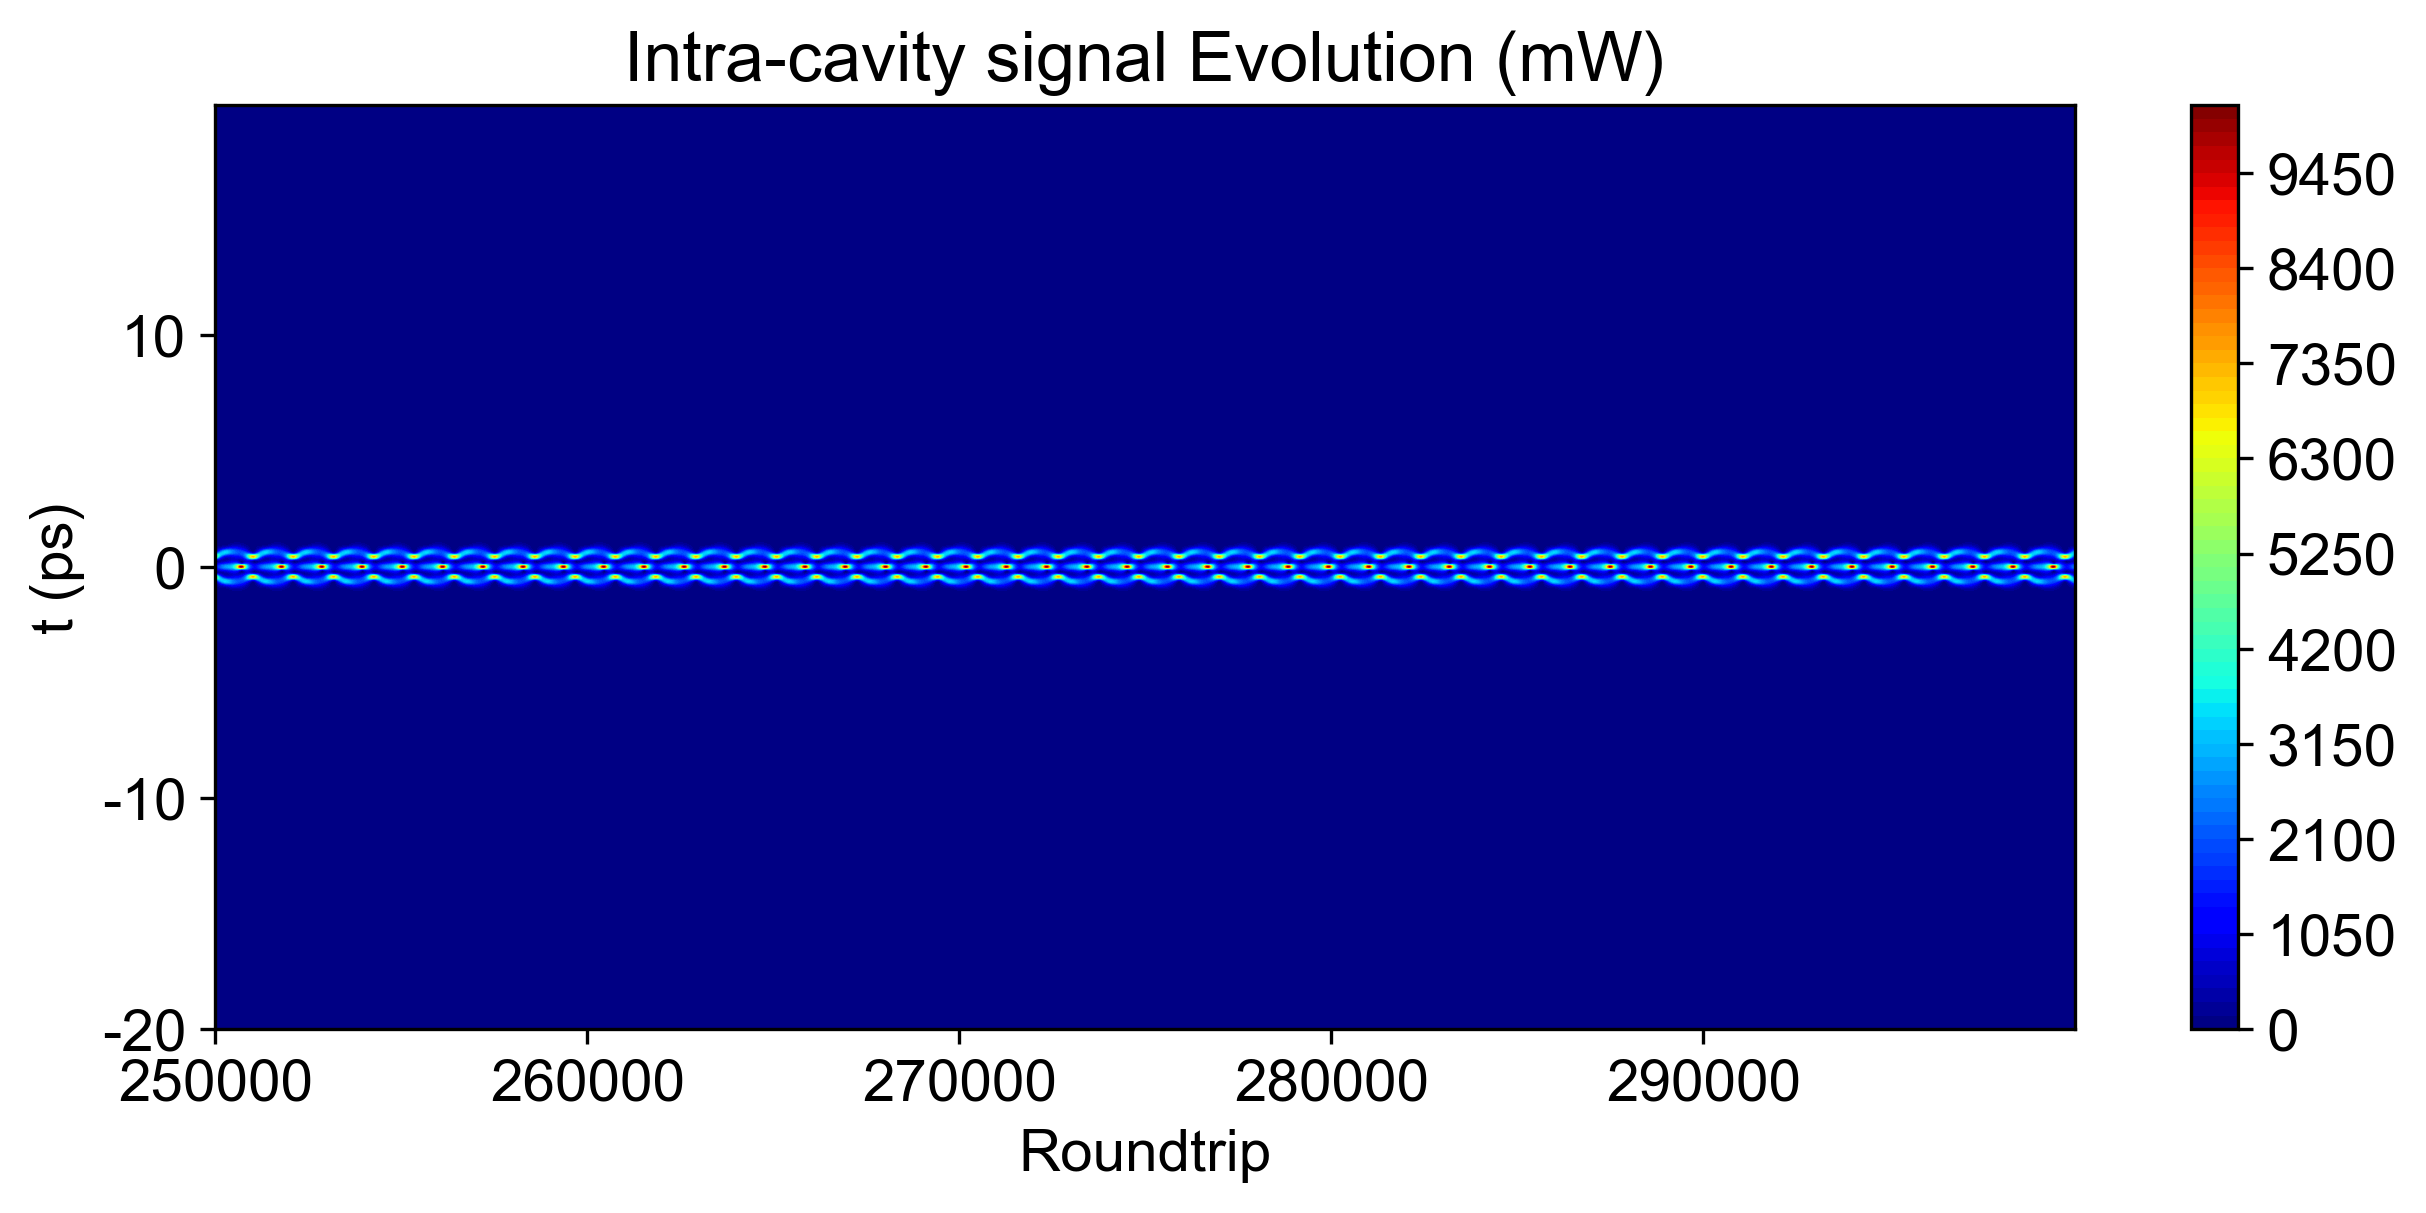
\includegraphics[width=0.48\linewidth]{figure/fig_13.png}
    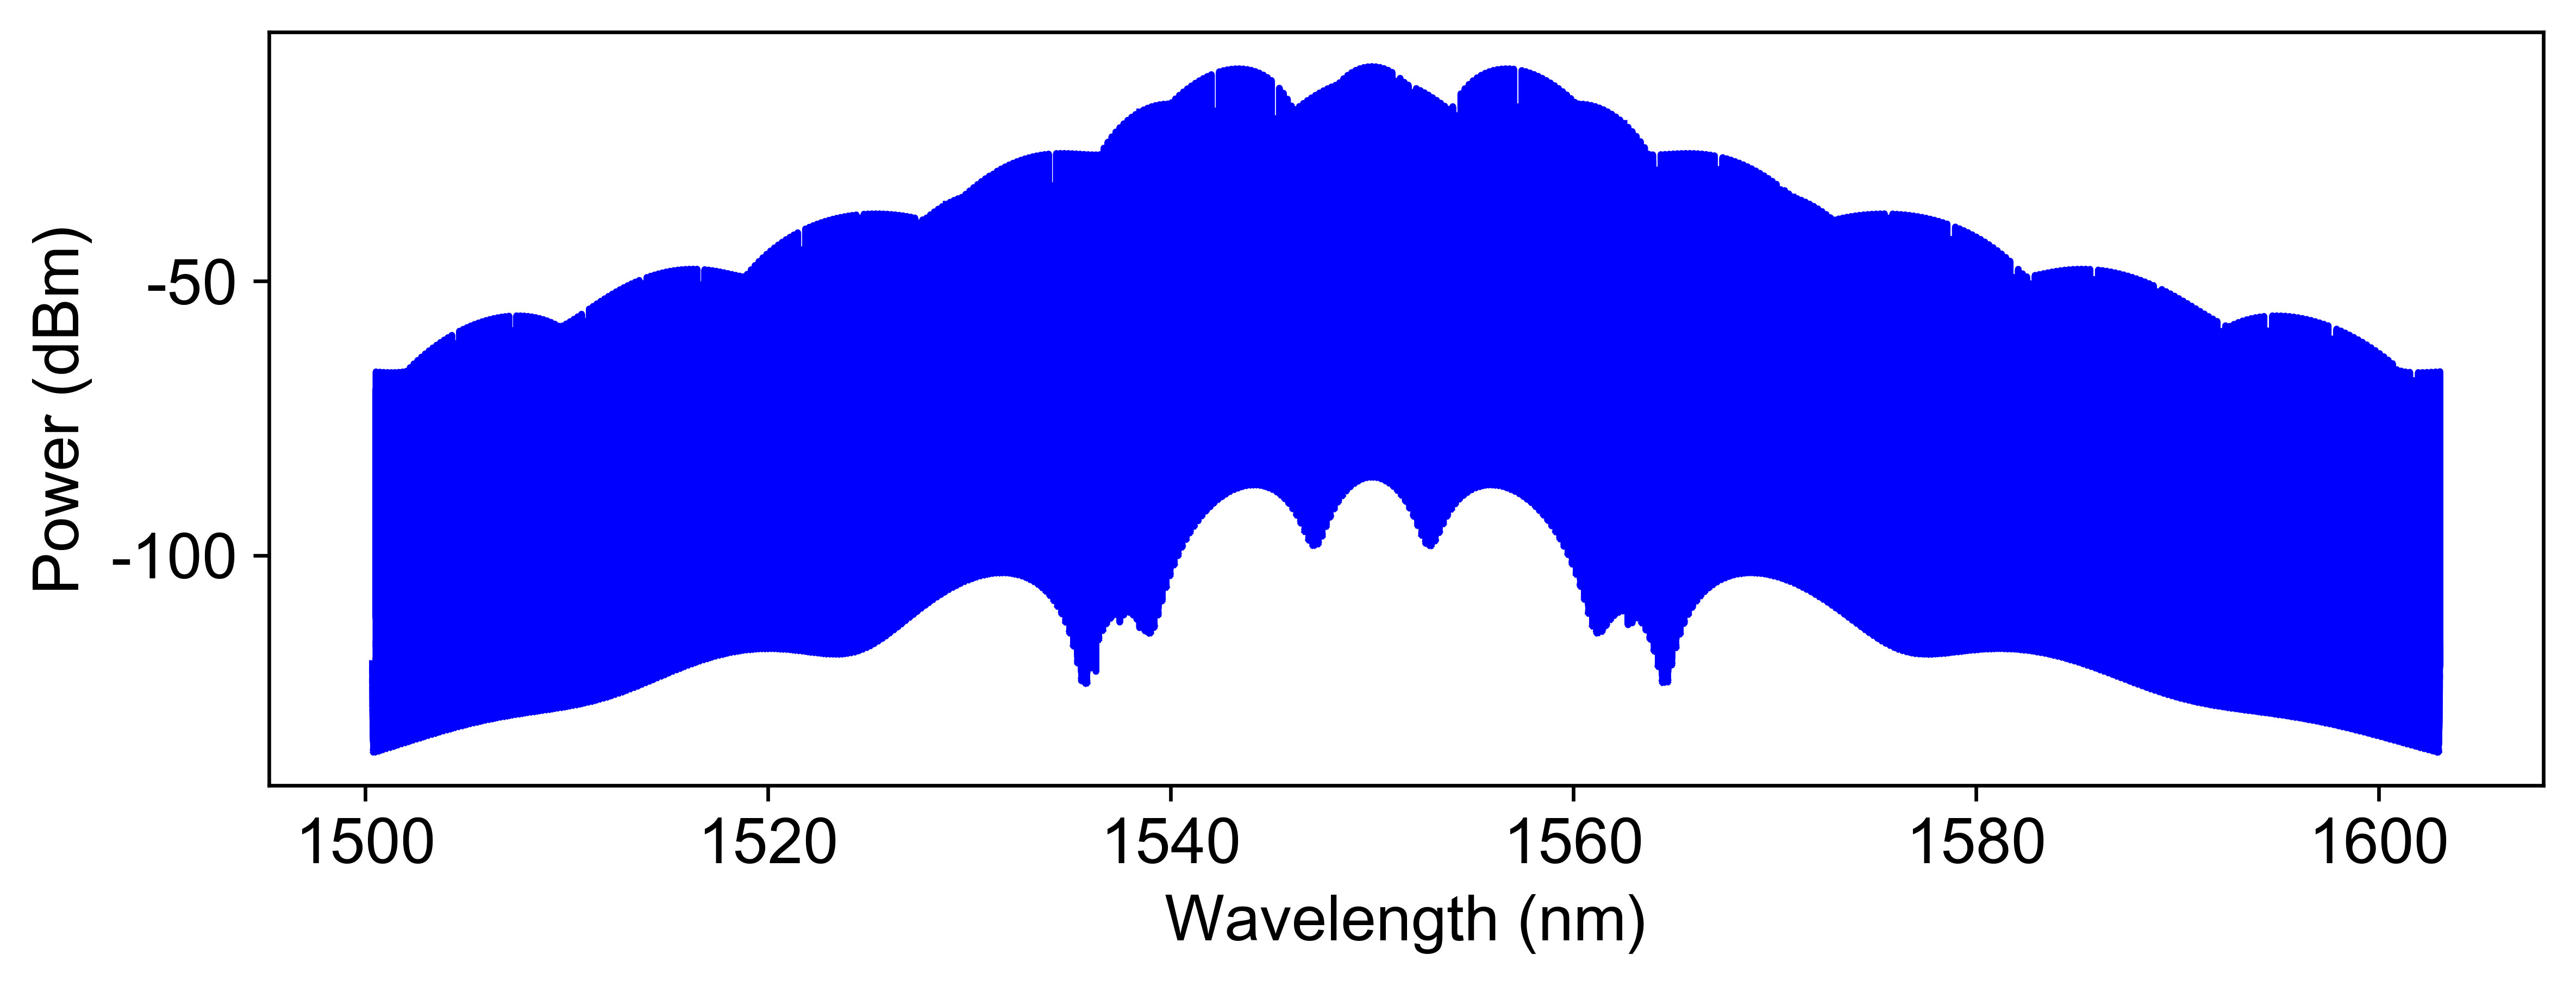
\includegraphics[width=0.48\linewidth]{figure/fig_13_0.png}
    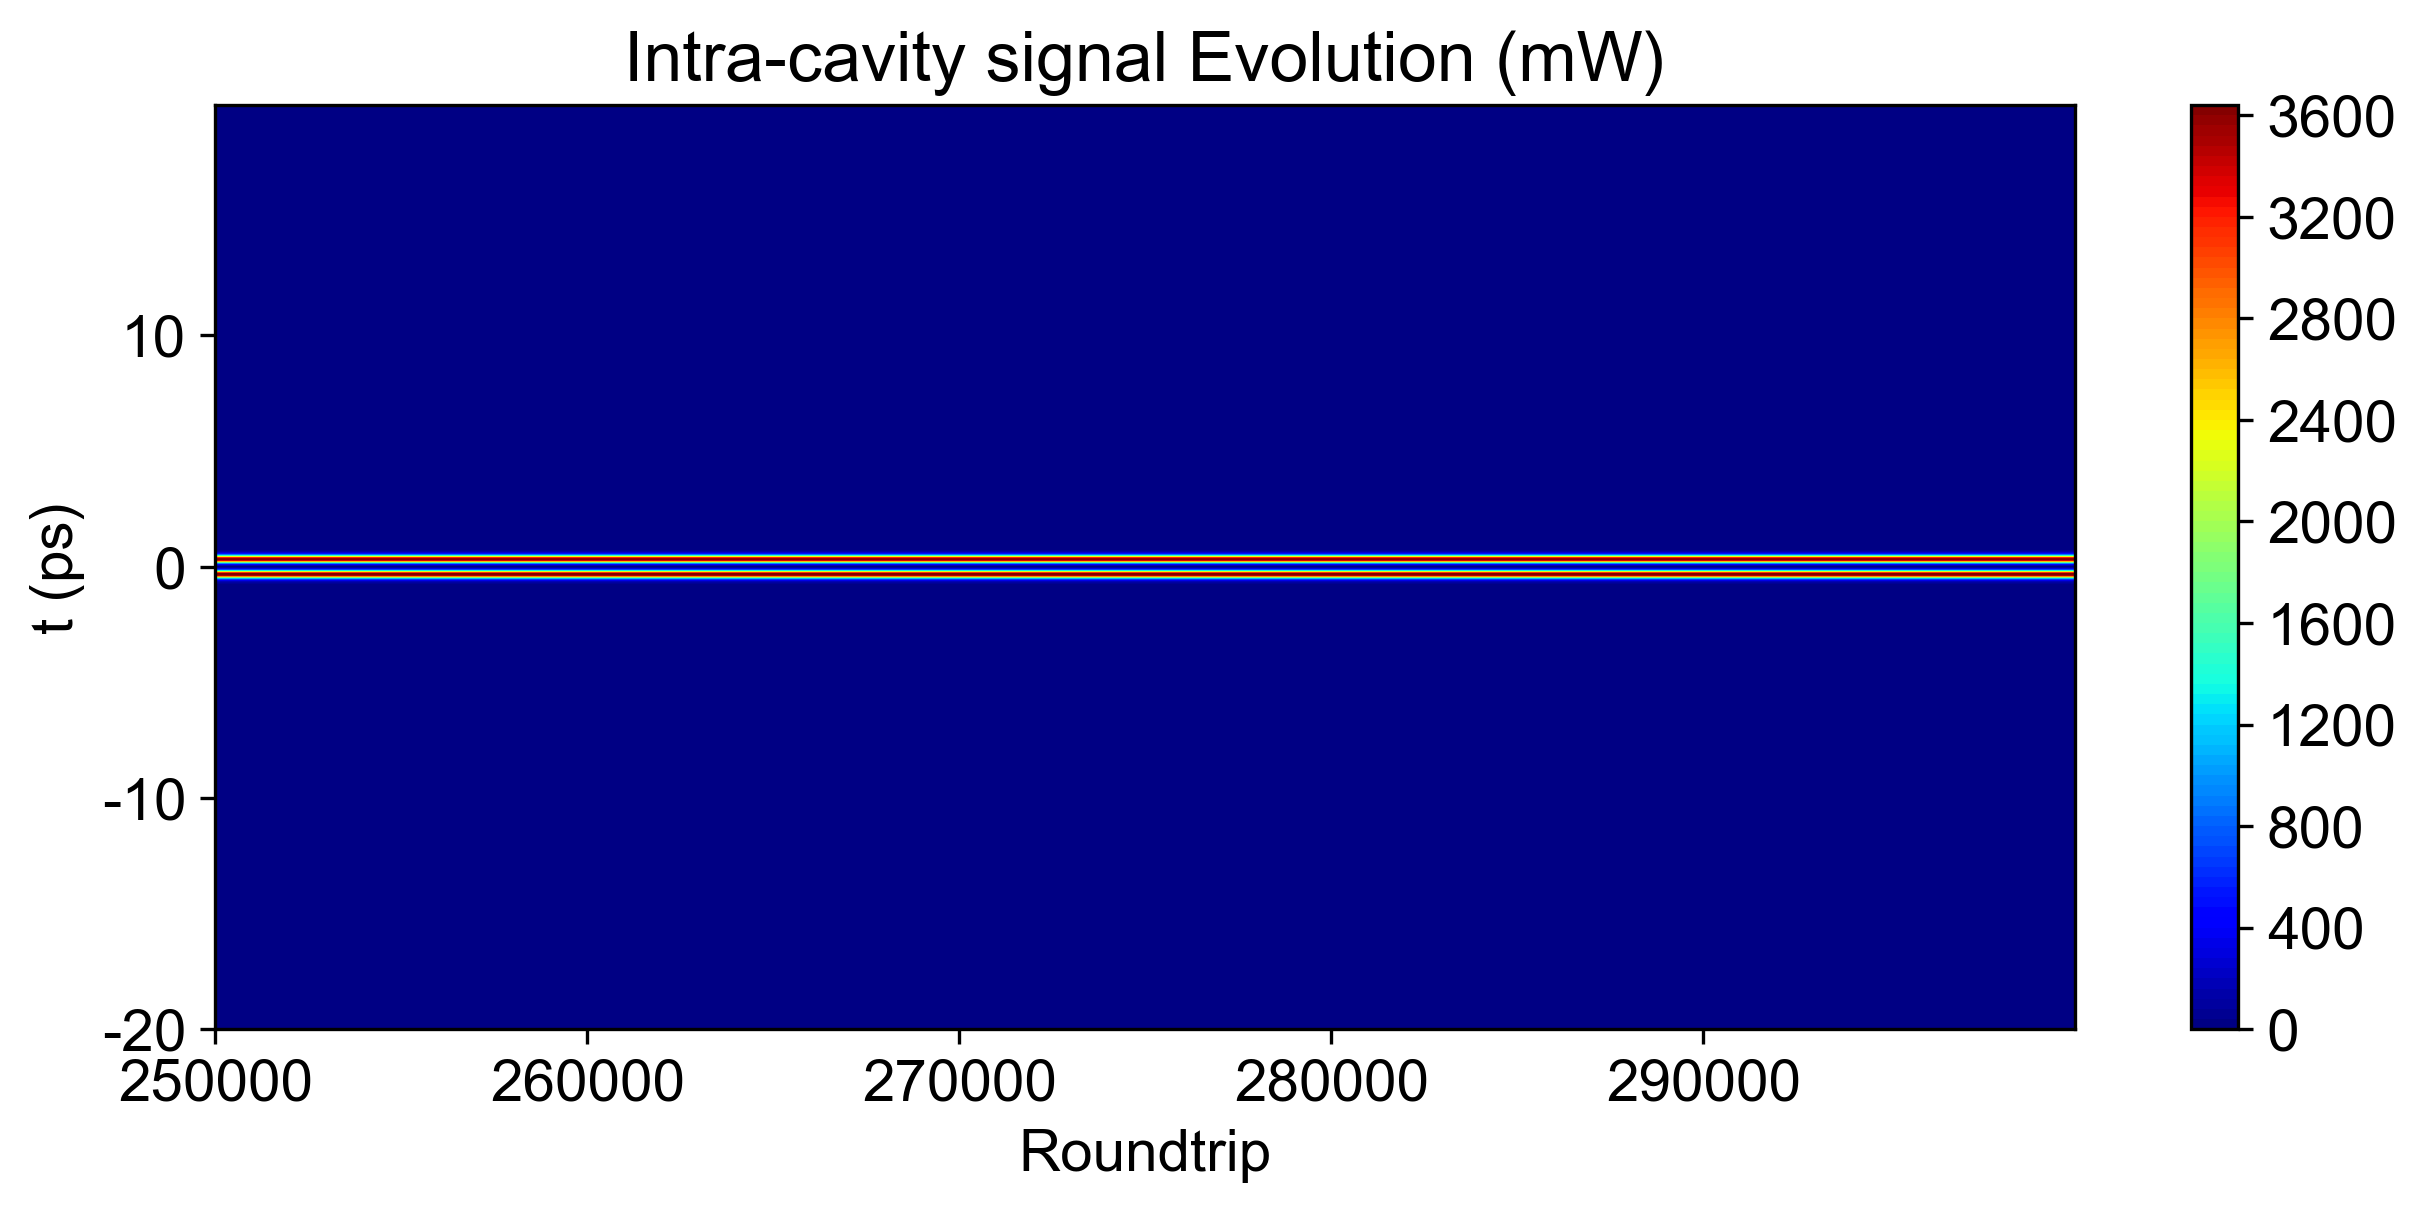
\includegraphics[width=0.48\linewidth]{figure/fig_14.png}
    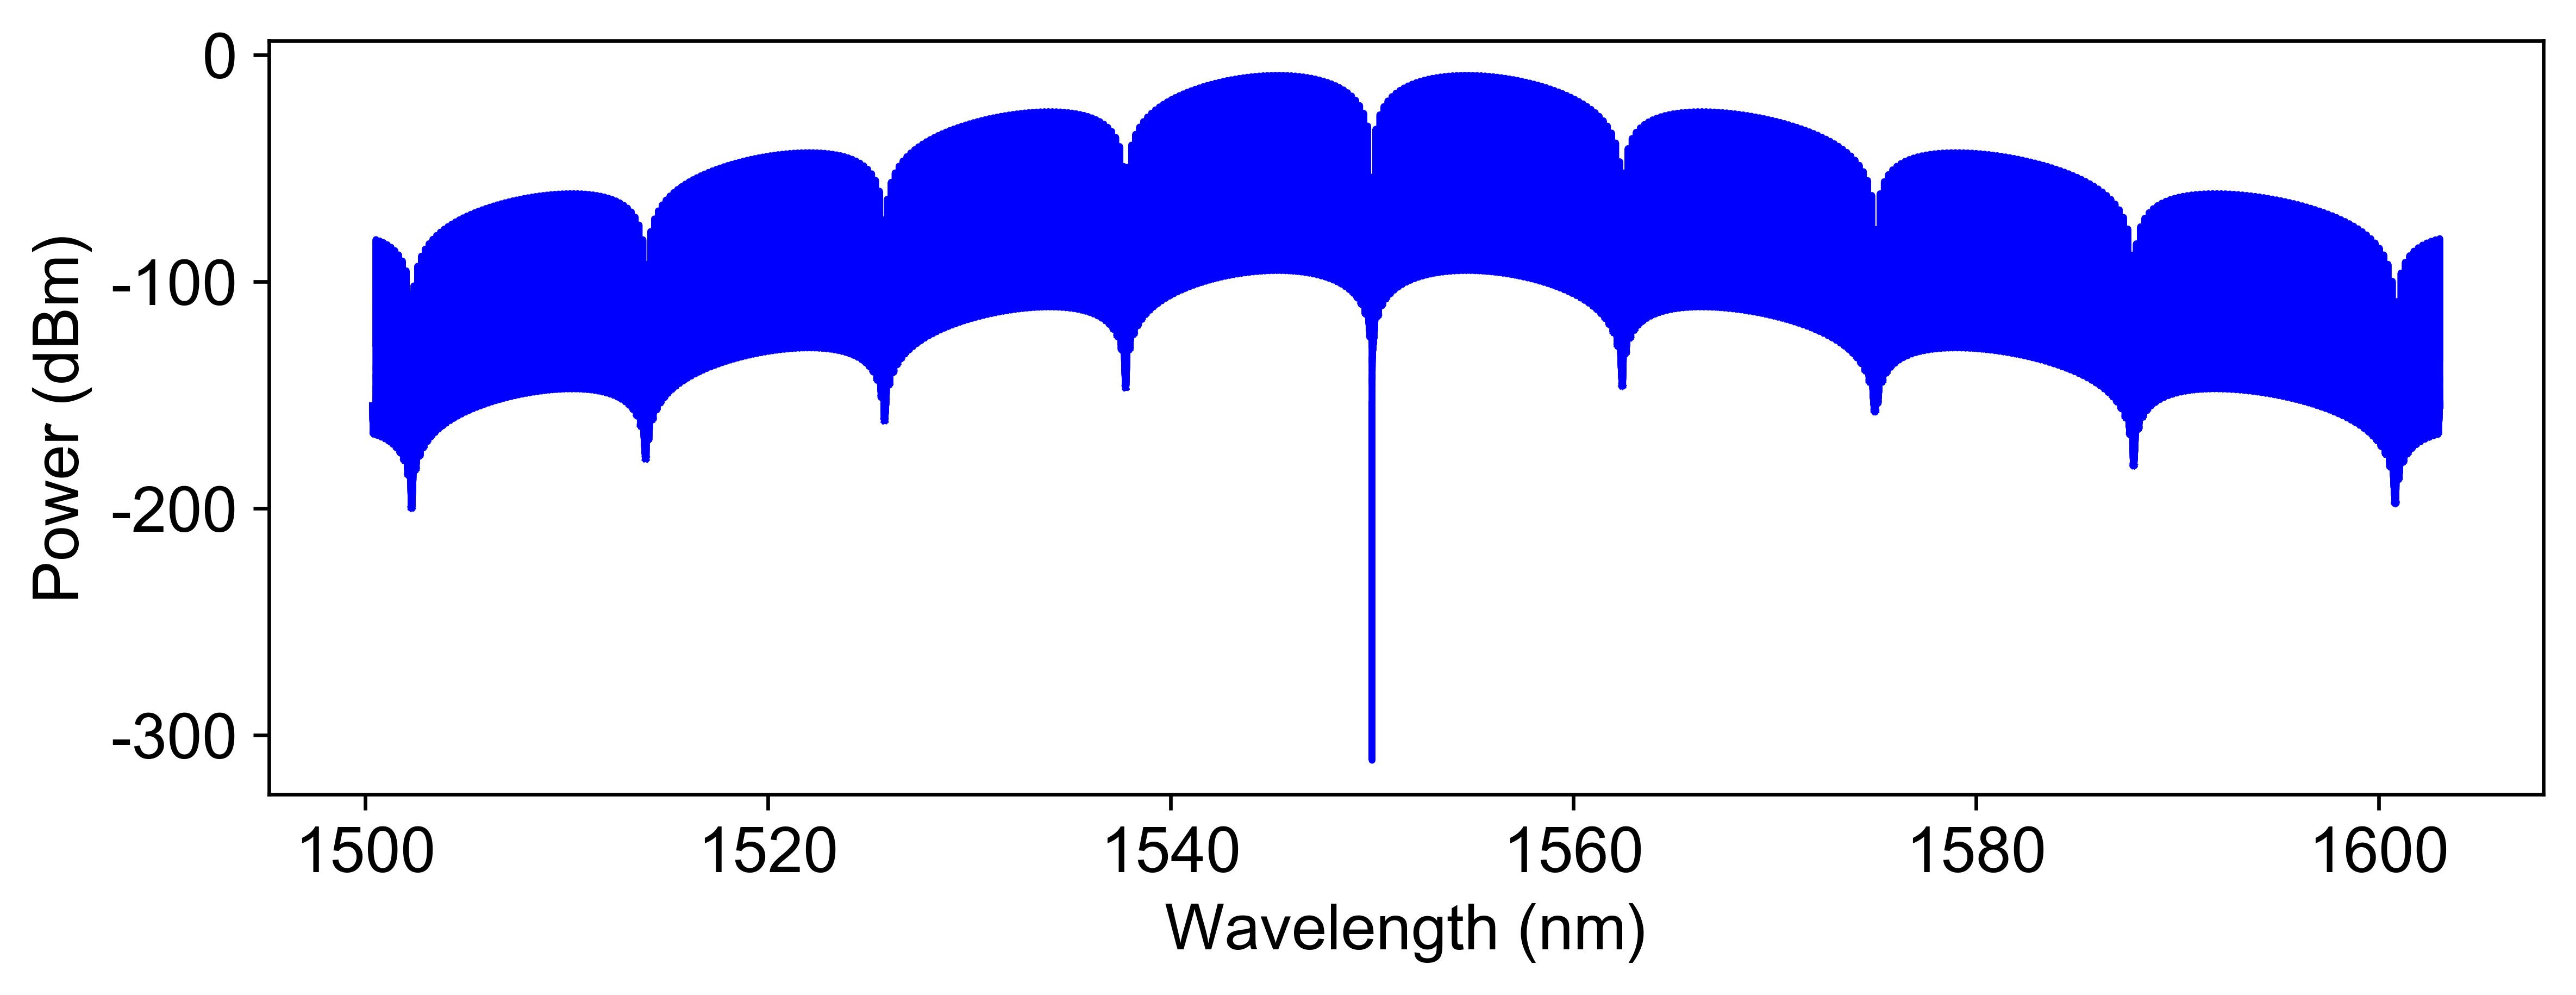
\includegraphics[width=0.48\linewidth]{figure/fig_14_0.png}
    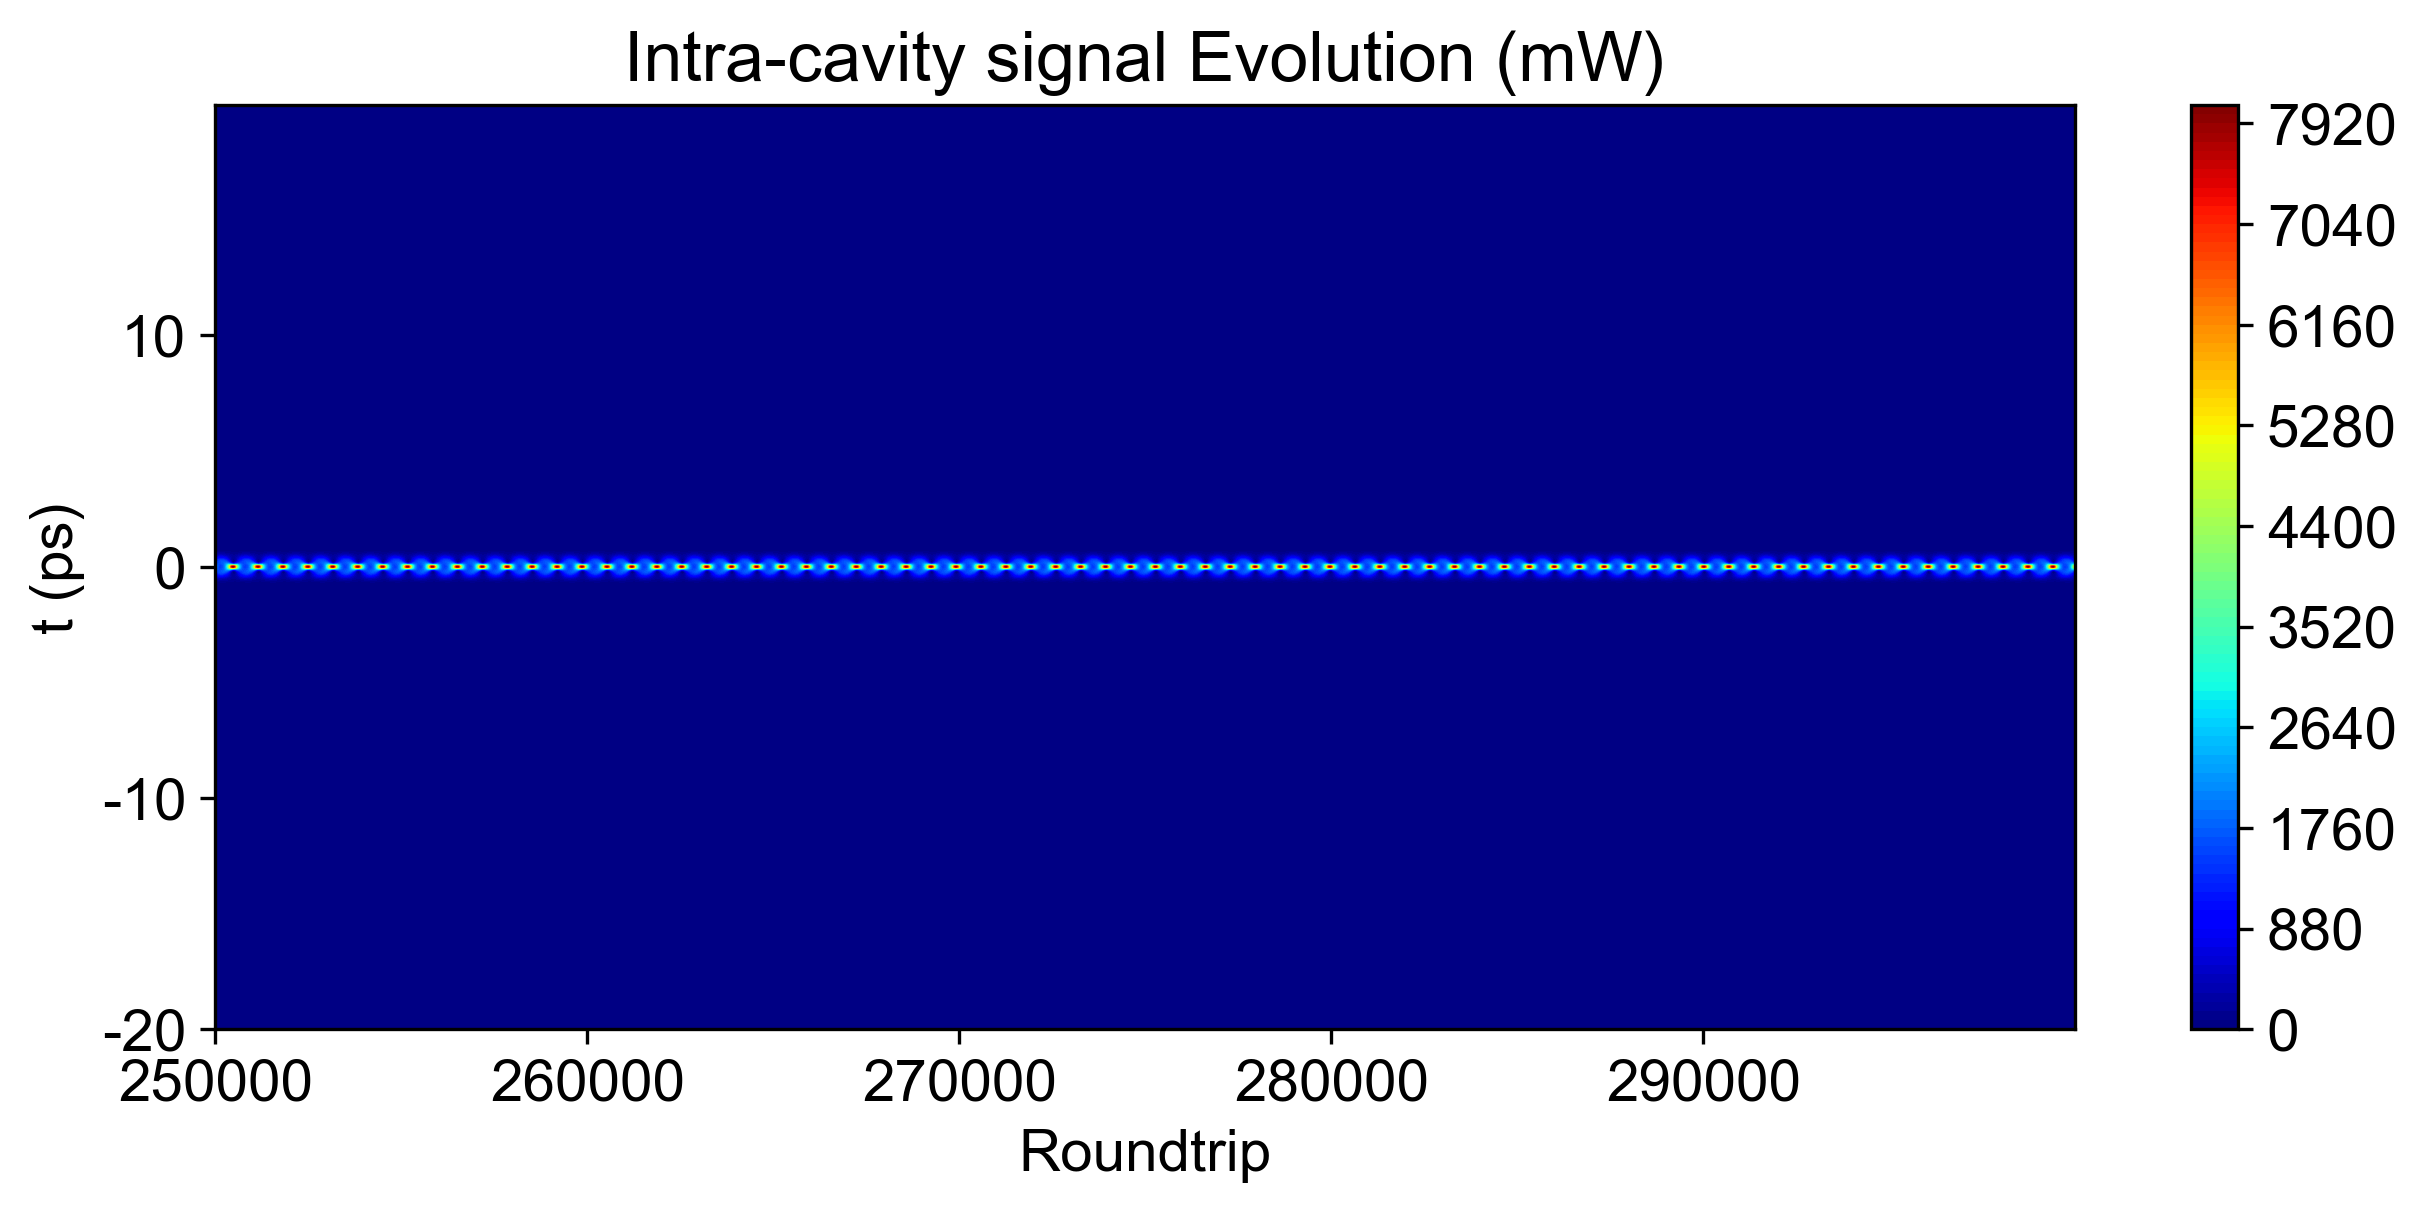
\includegraphics[width=0.48\linewidth]{figure/fig_15.png}
    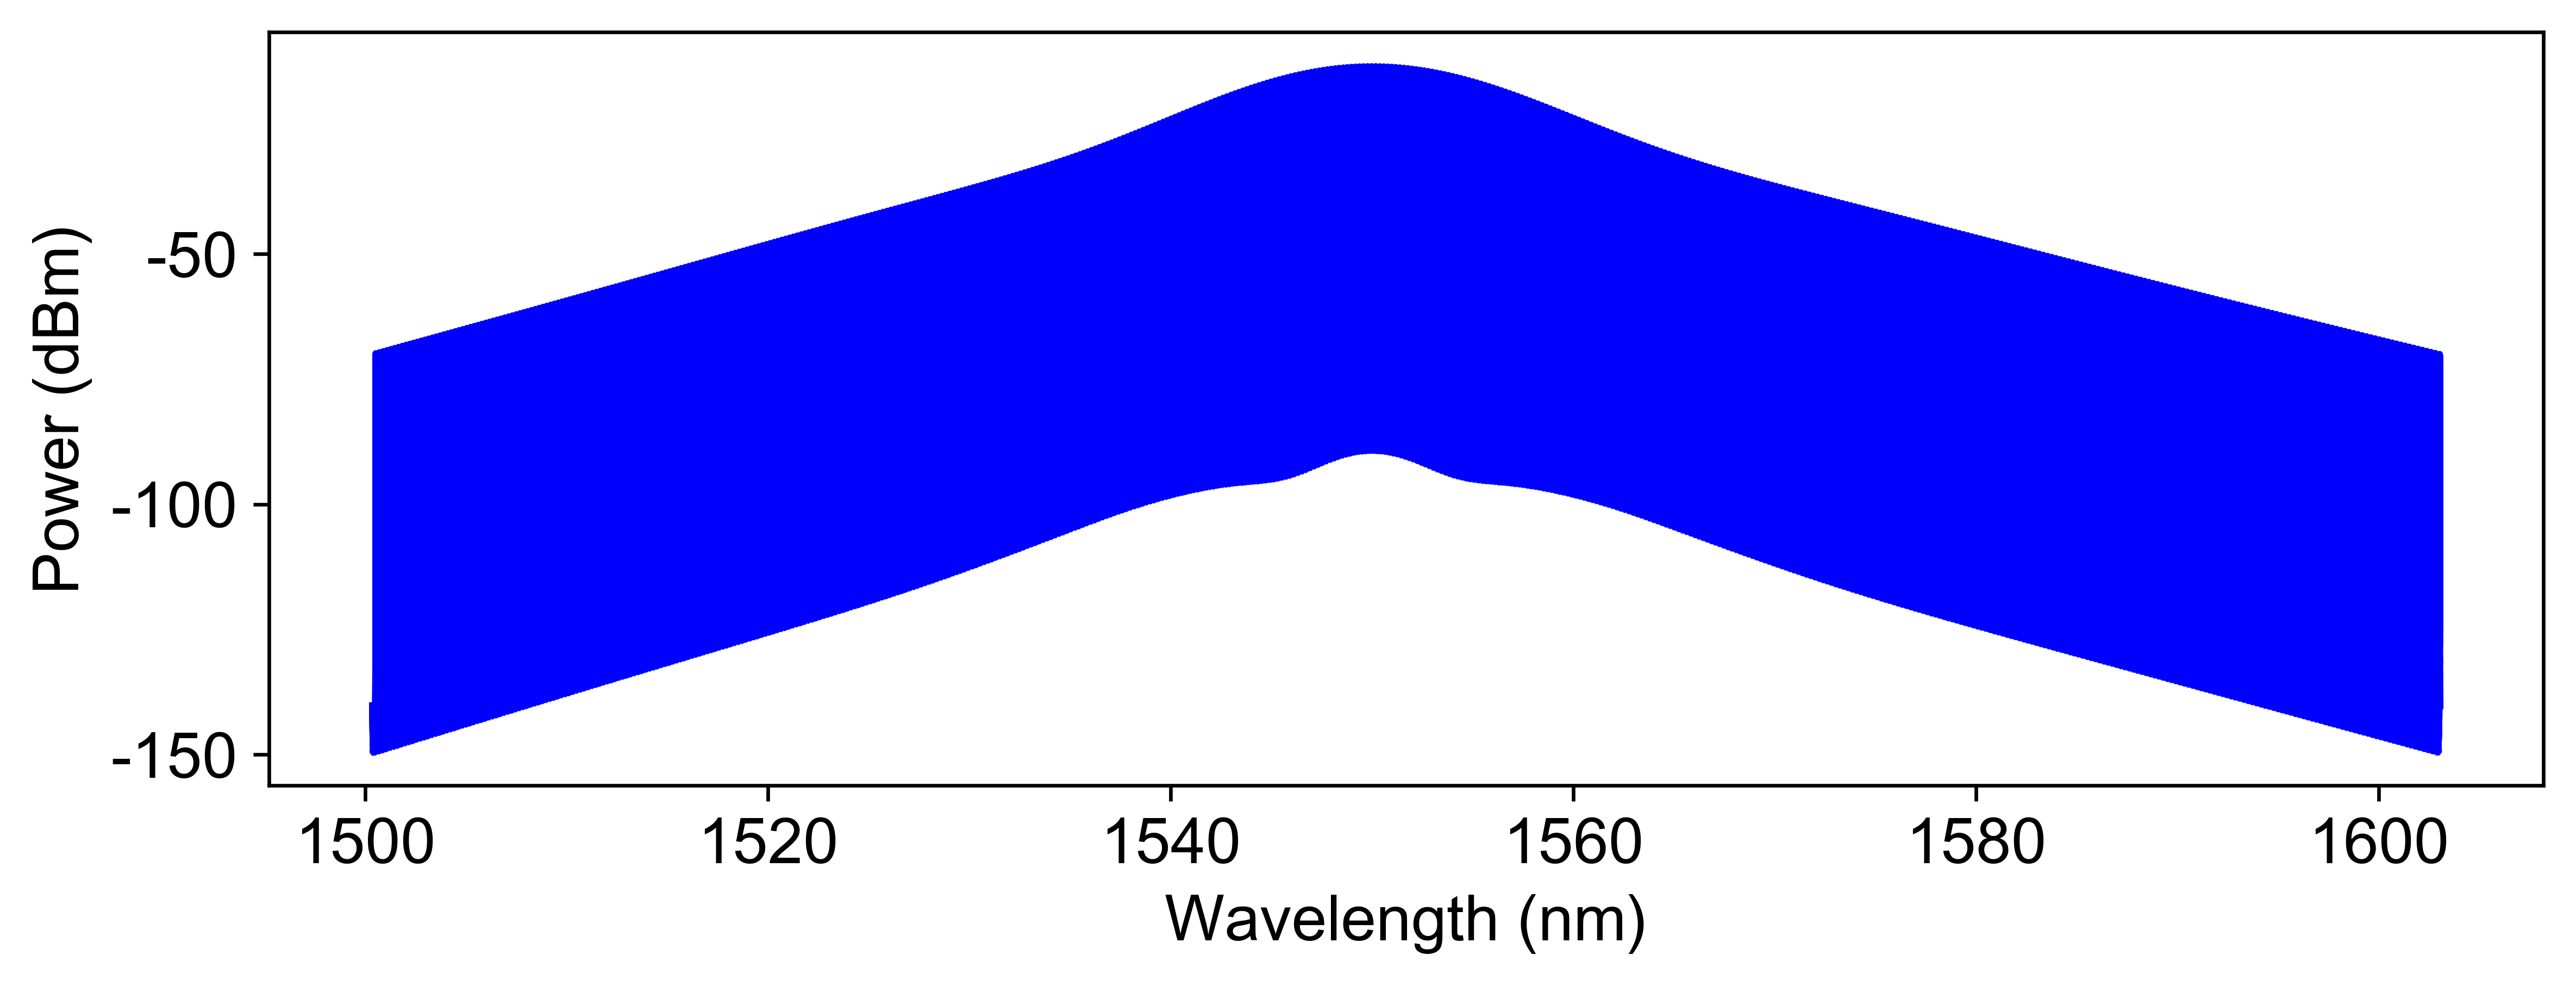
\includegraphics[width=0.48\linewidth]{figure/fig_15_0.png}
    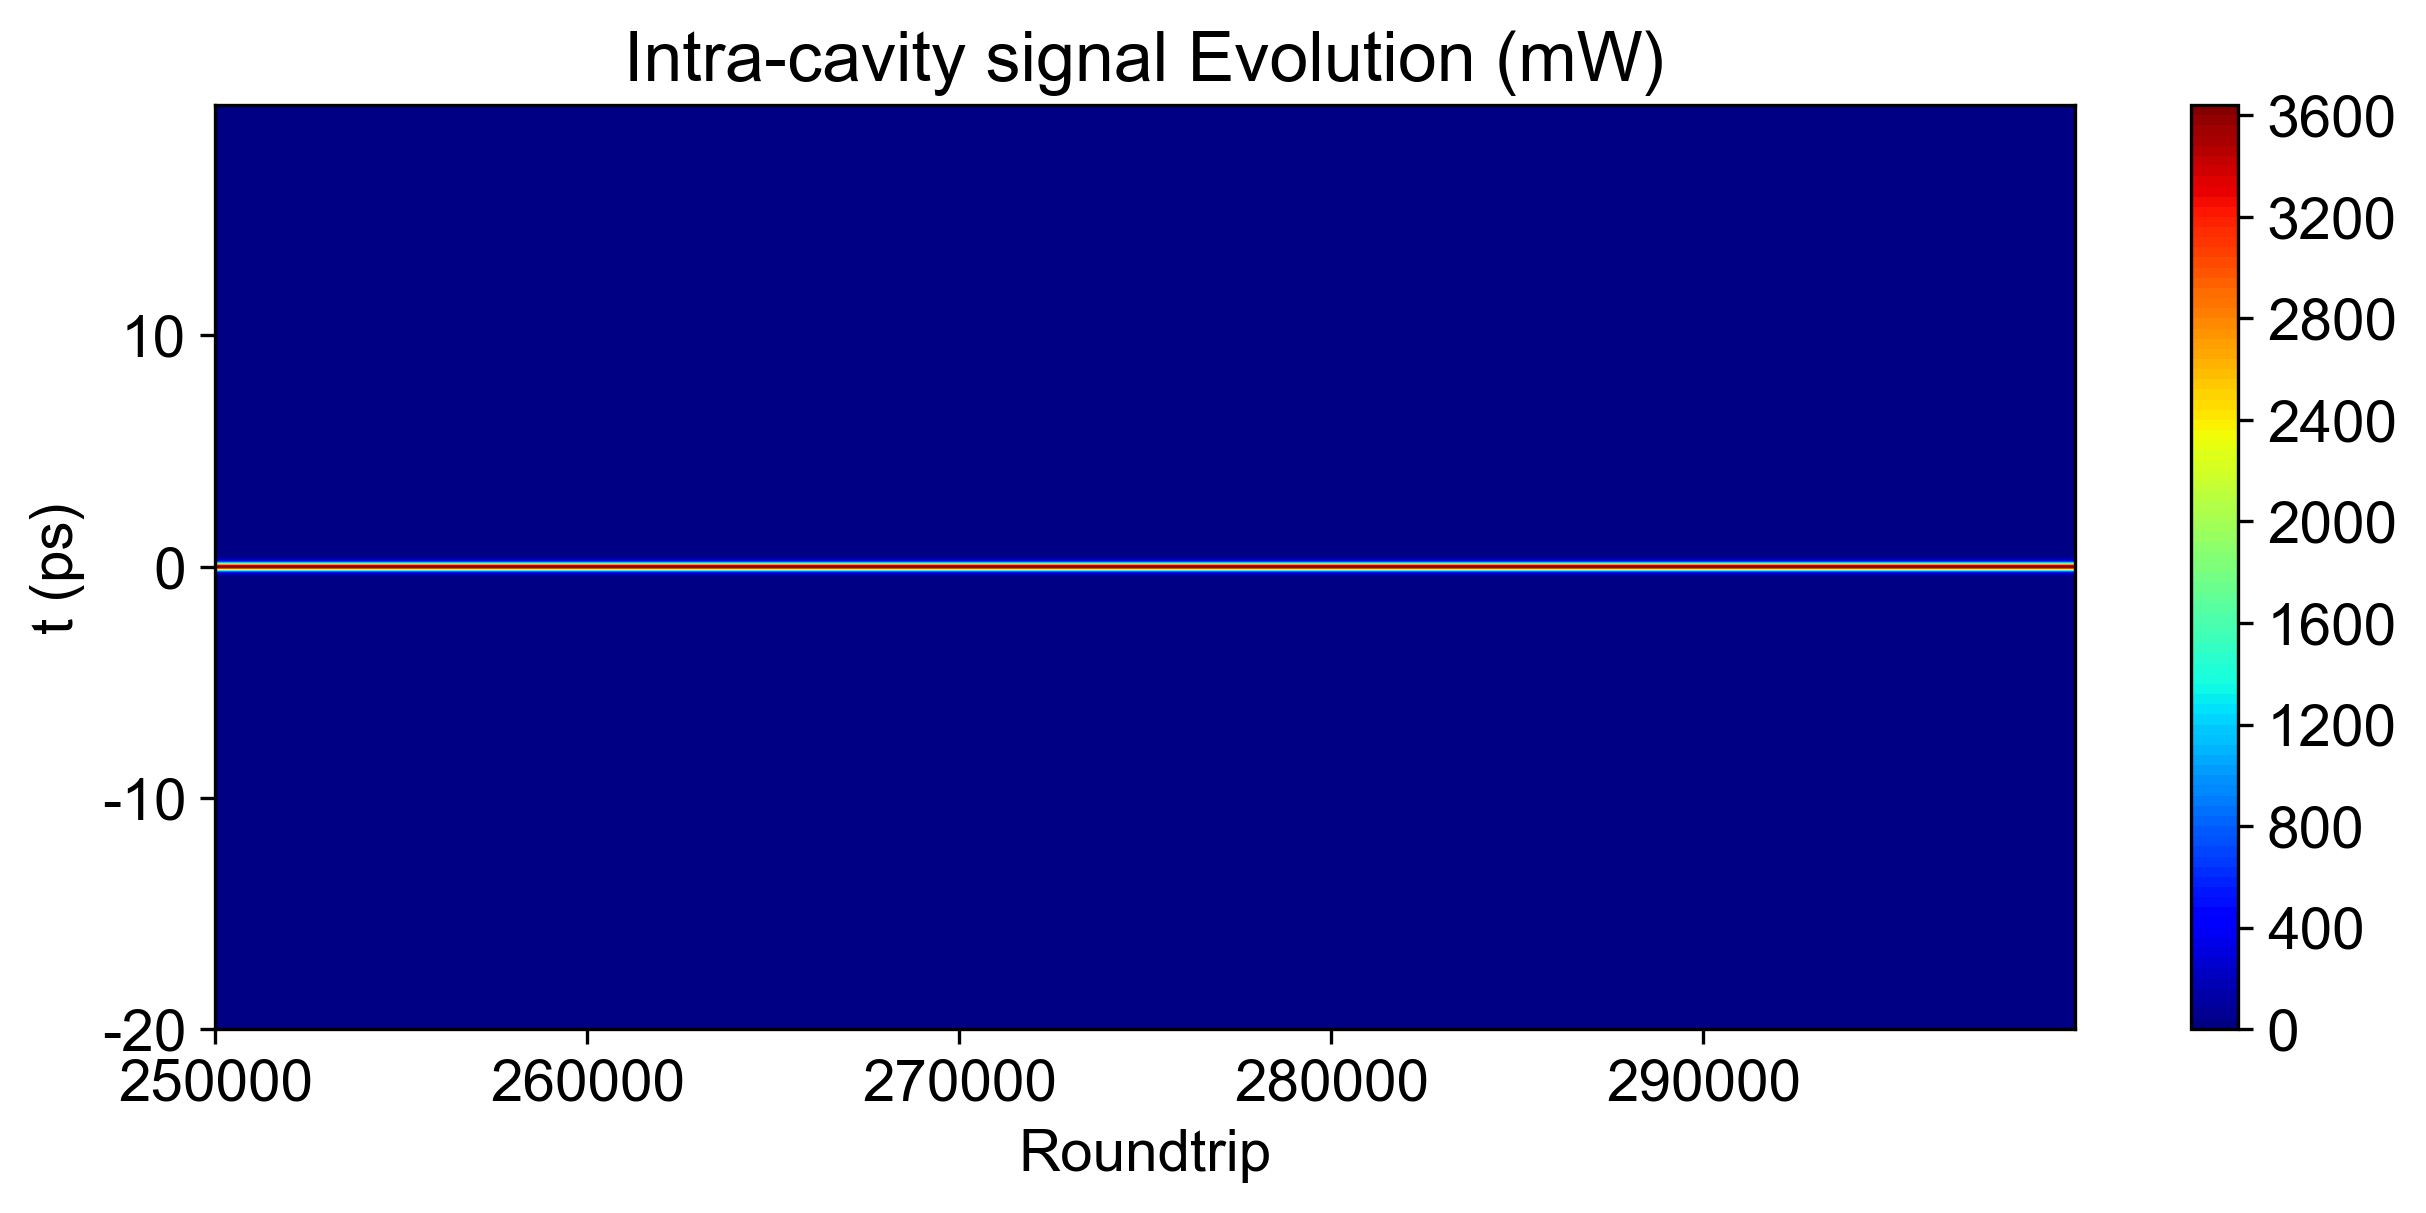
\includegraphics[width=0.48\linewidth]{figure/fig_16.png}
    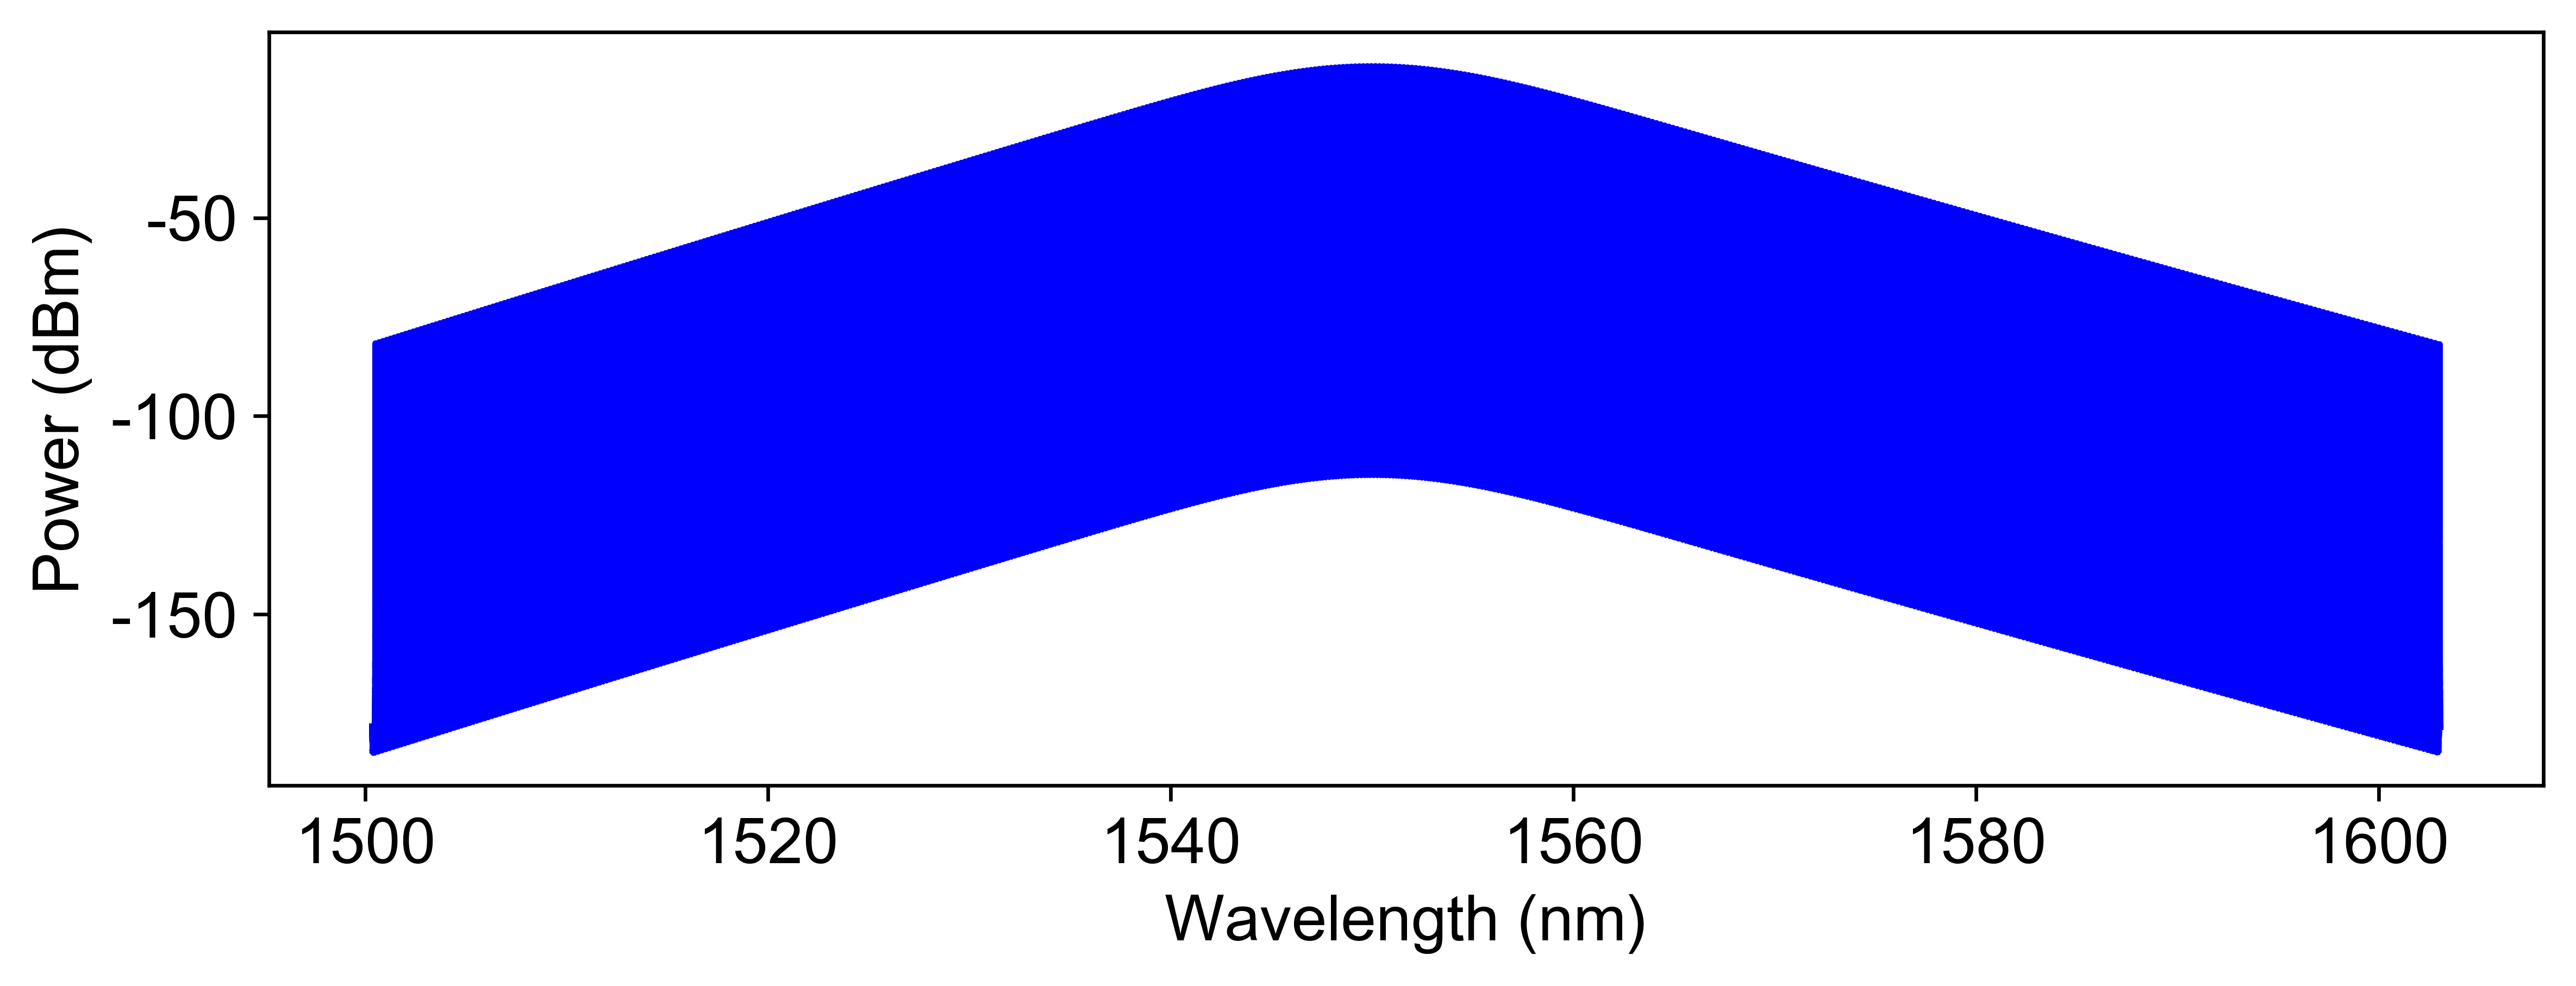
\includegraphics[width=0.48\linewidth]{figure/fig_16_0.png}
    \caption{左列:腔内信号光场的稳态,对应的光谱。从上到下调制深度依次为:0.1,0.3,0.5,0.7,1.0。}
    \label{fig:enter-label}
\end{figure}
调制深度越大,越接近锁模态。
\subsection{泵浦光功率}
以$FSR = 25GHz$,调制深度$M = 0.5$,改变泵浦功率进行仿真。\\
\begin{figure}[htbp]
    \centering
    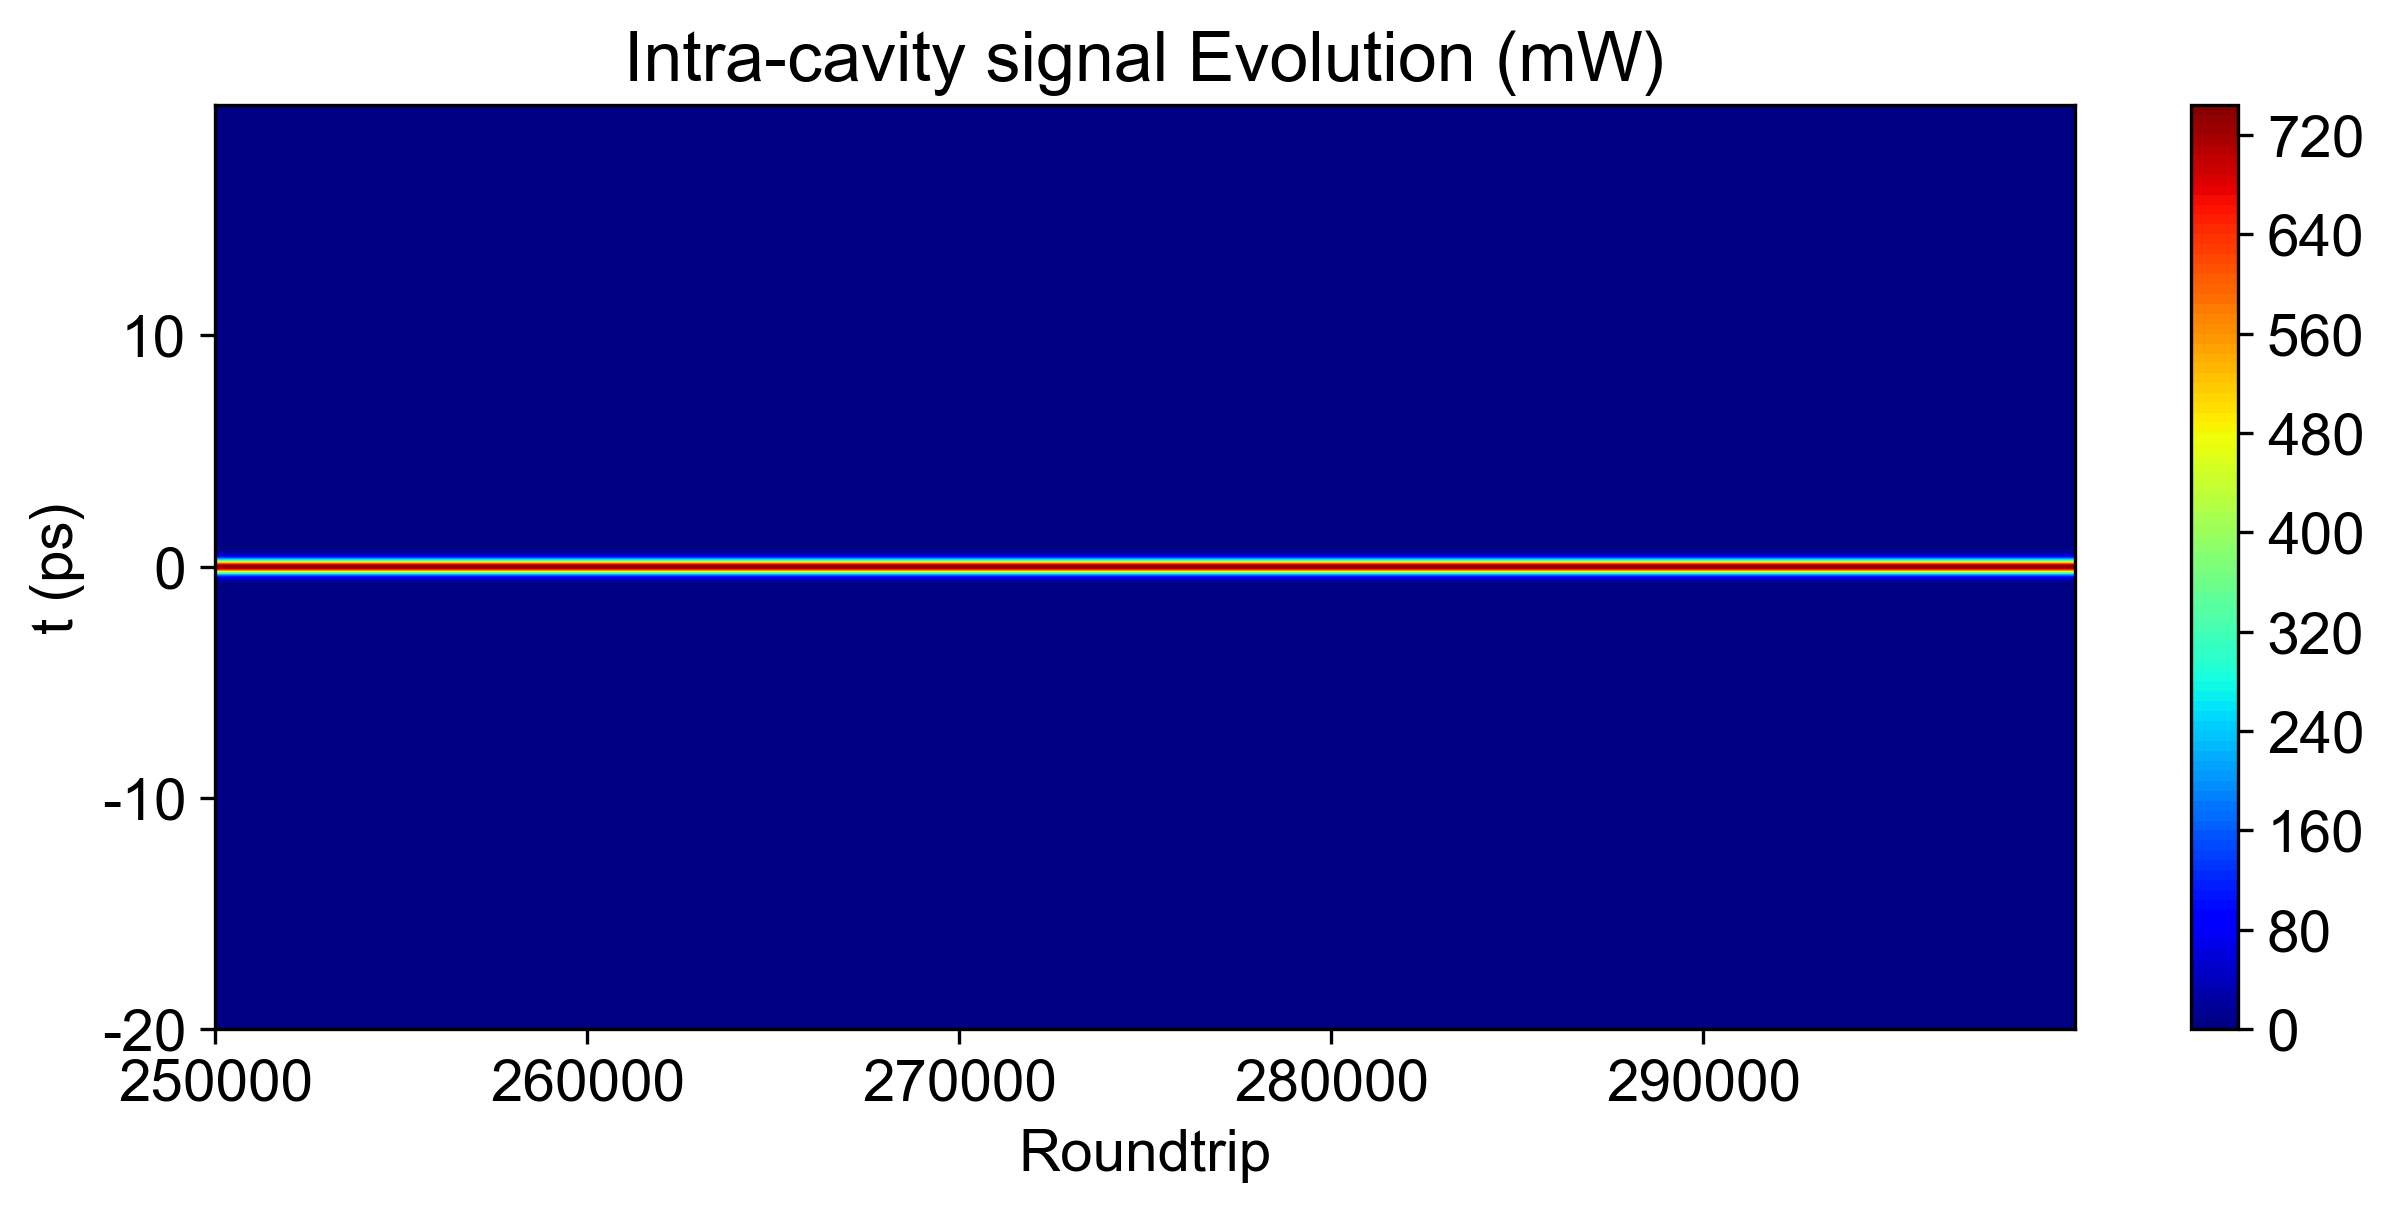
\includegraphics[width=0.48\linewidth]{figure/fig_17.png}
    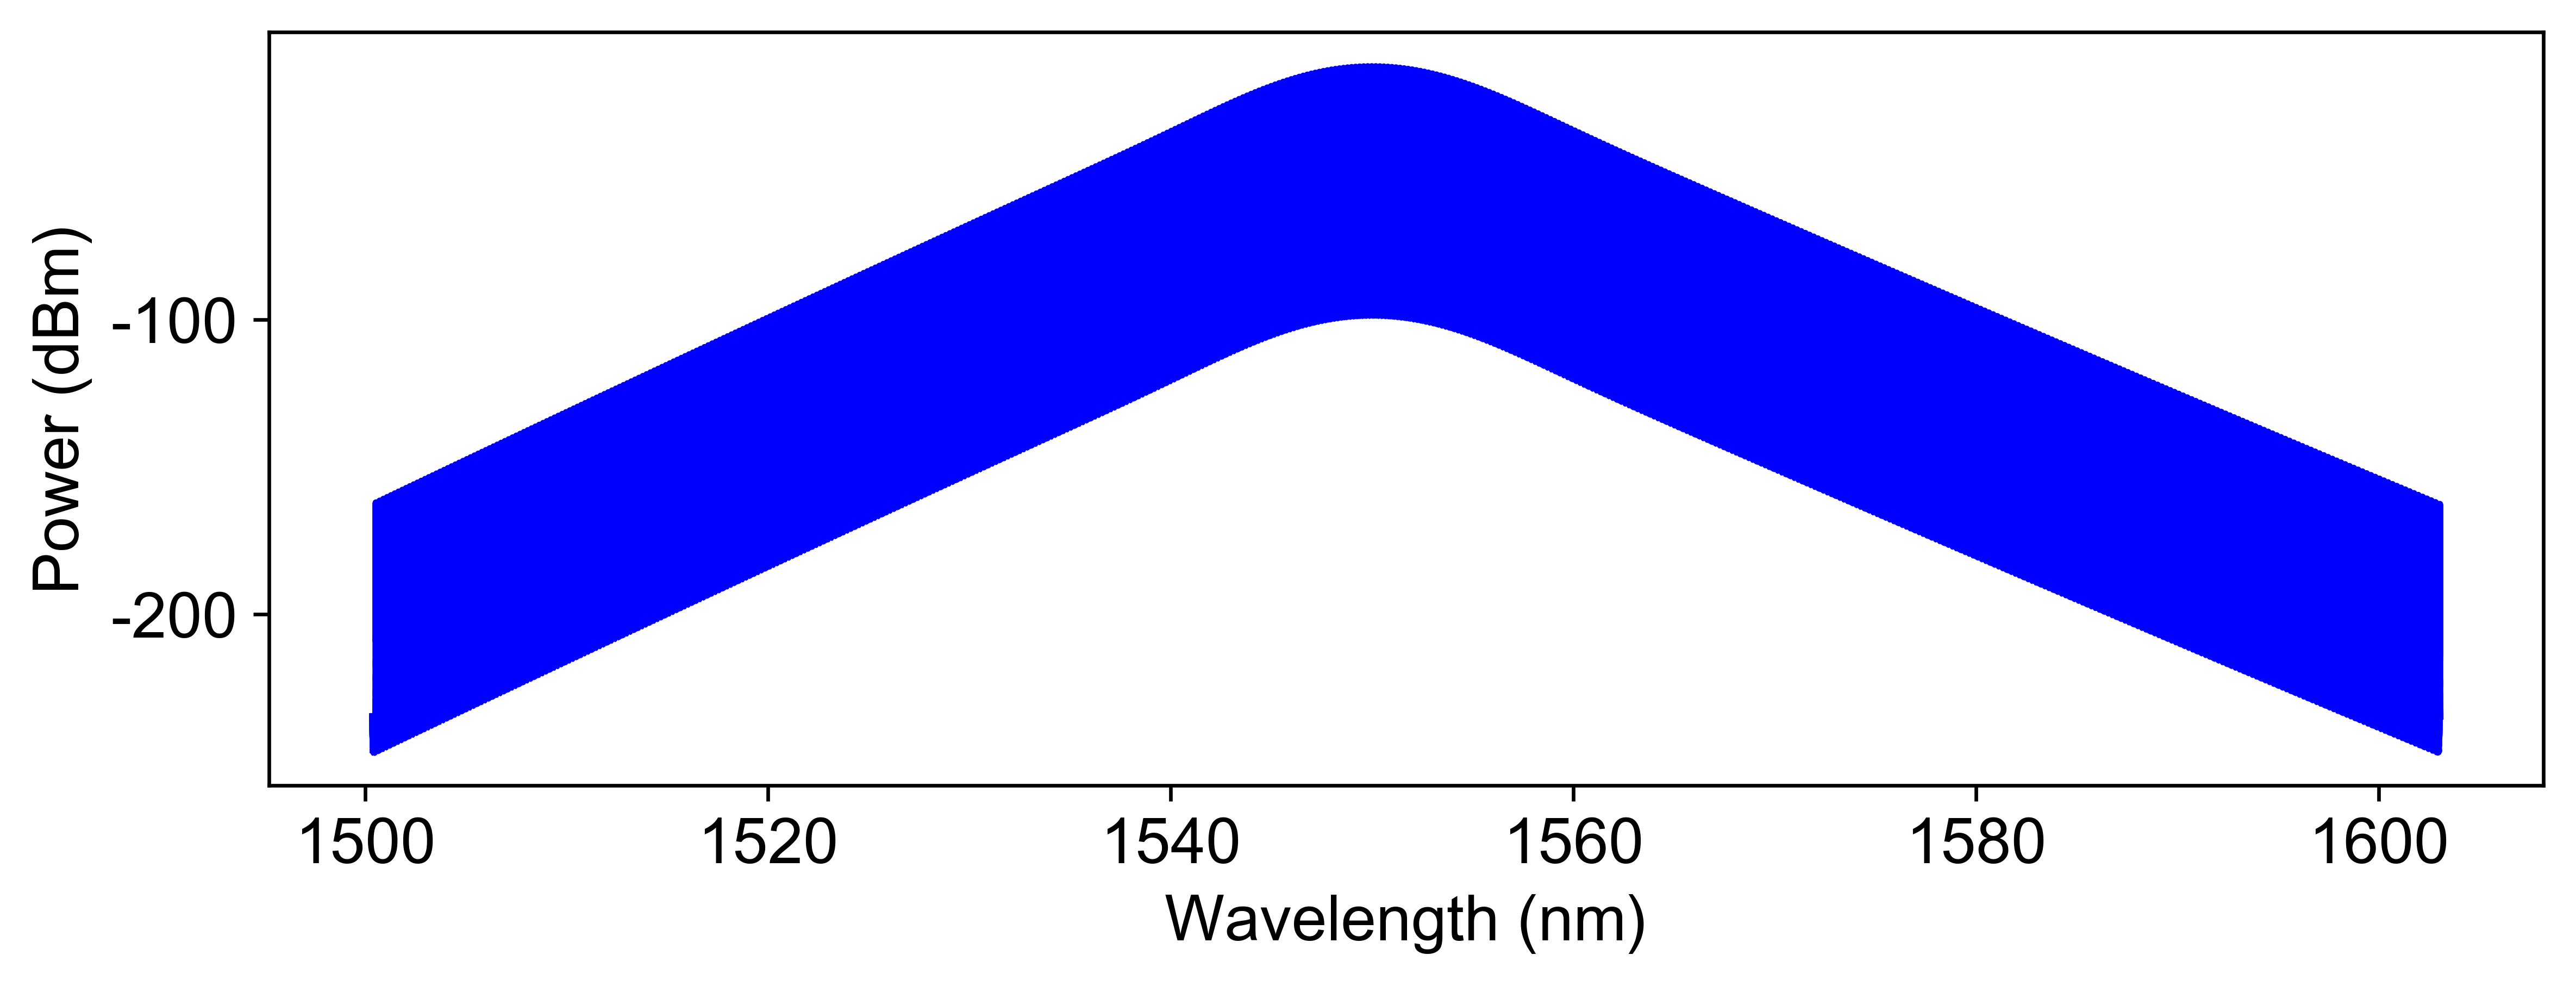
\includegraphics[width=0.48\linewidth]{figure/fig_17_0.png}
    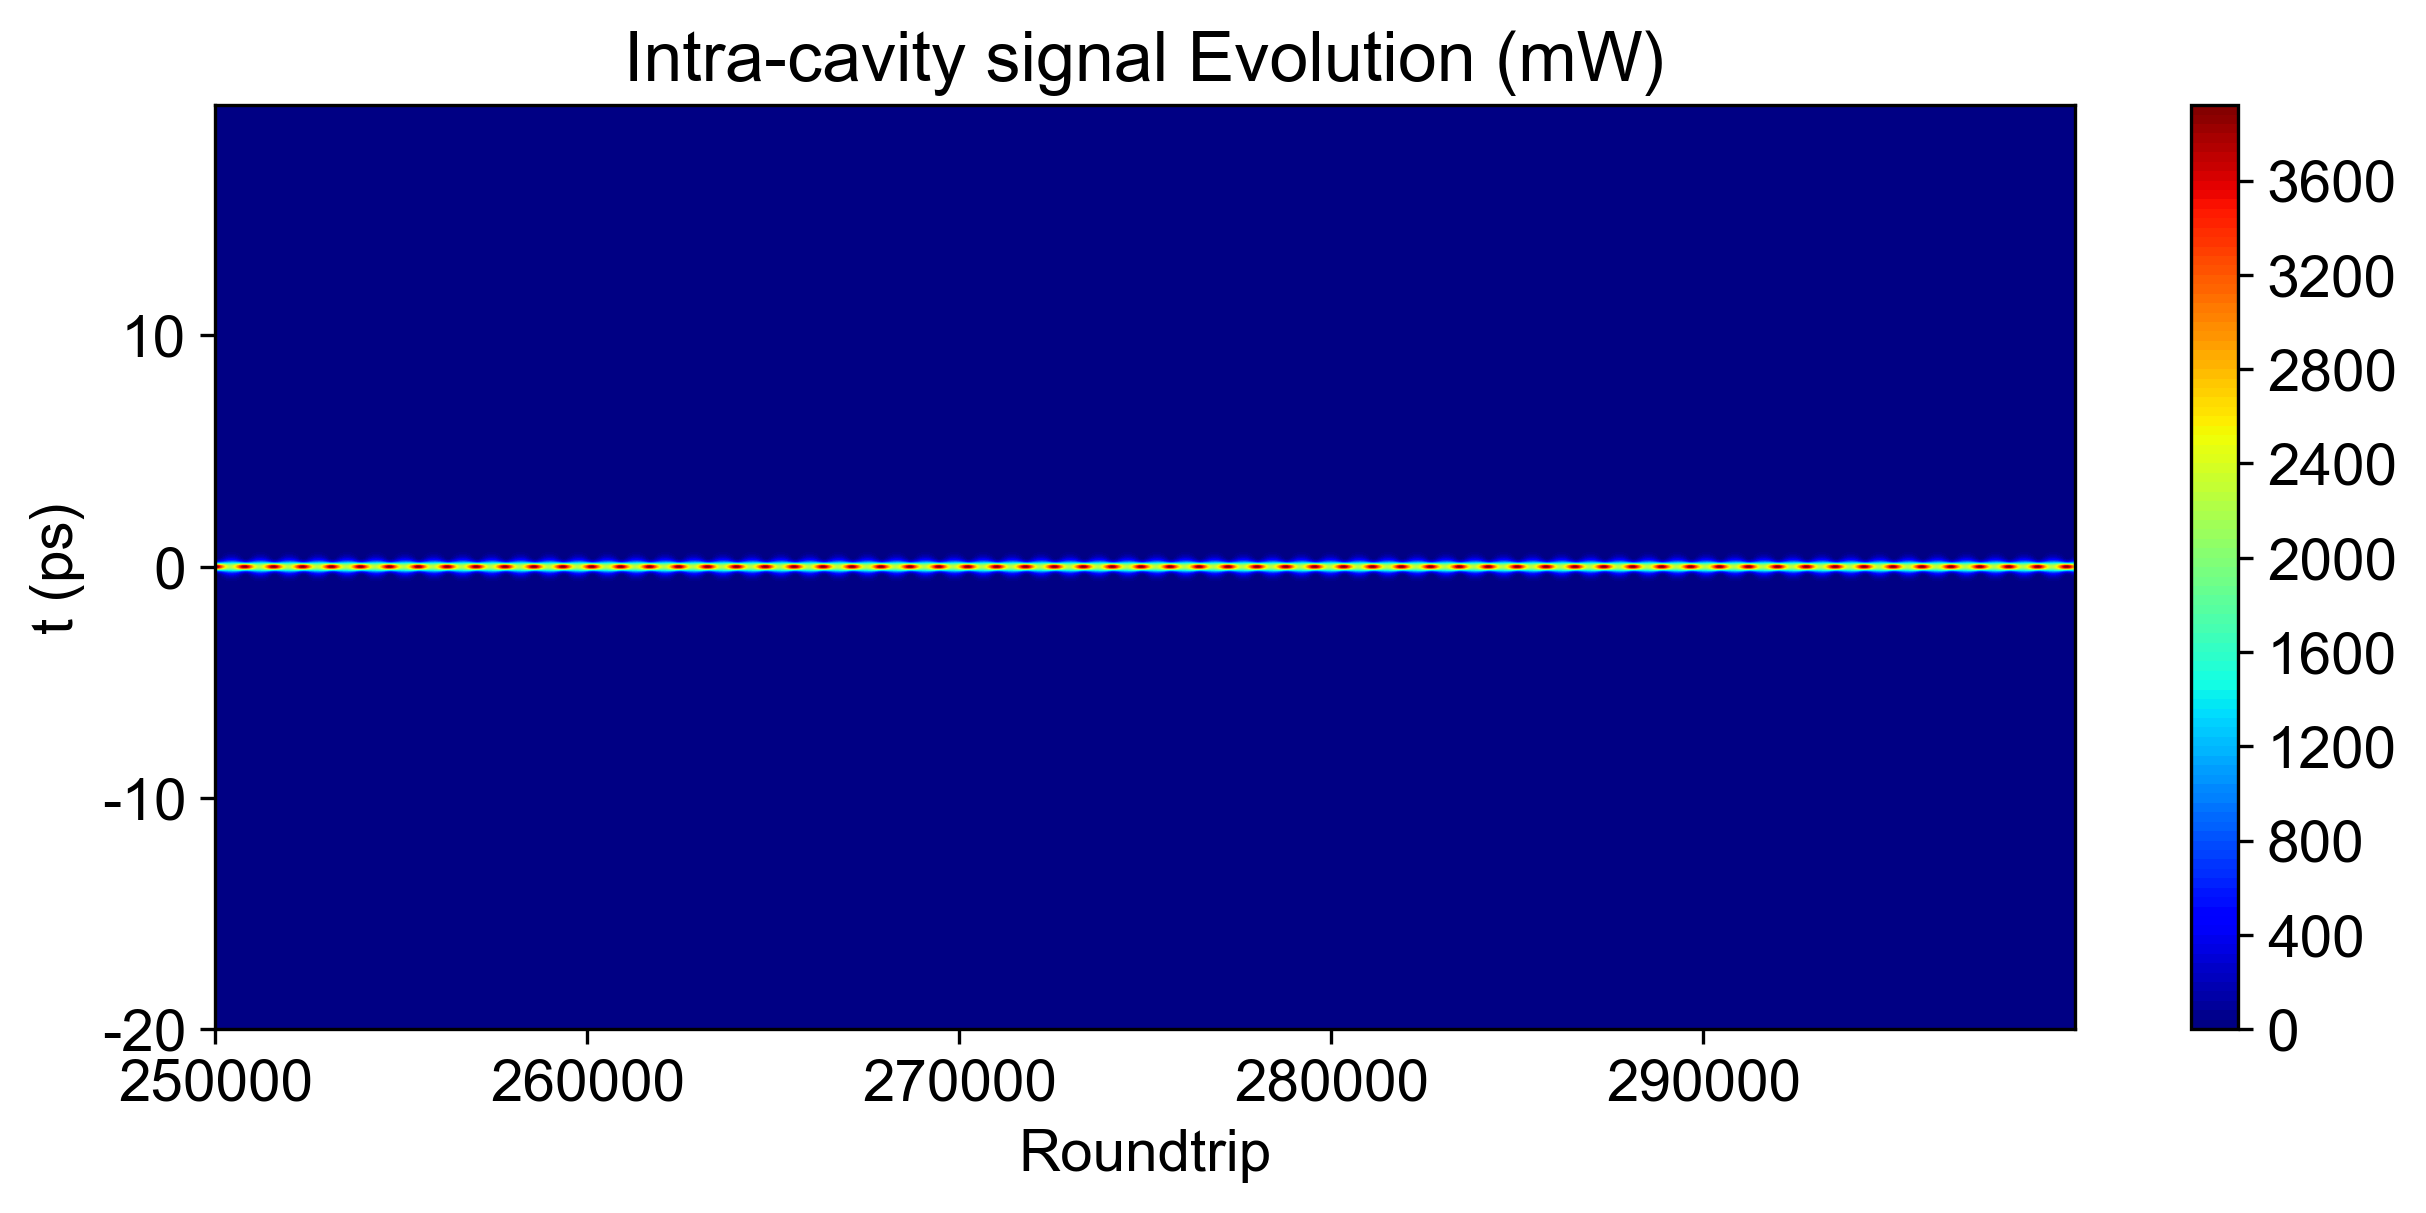
\includegraphics[width=0.48\linewidth]{figure/fig_18.png}
    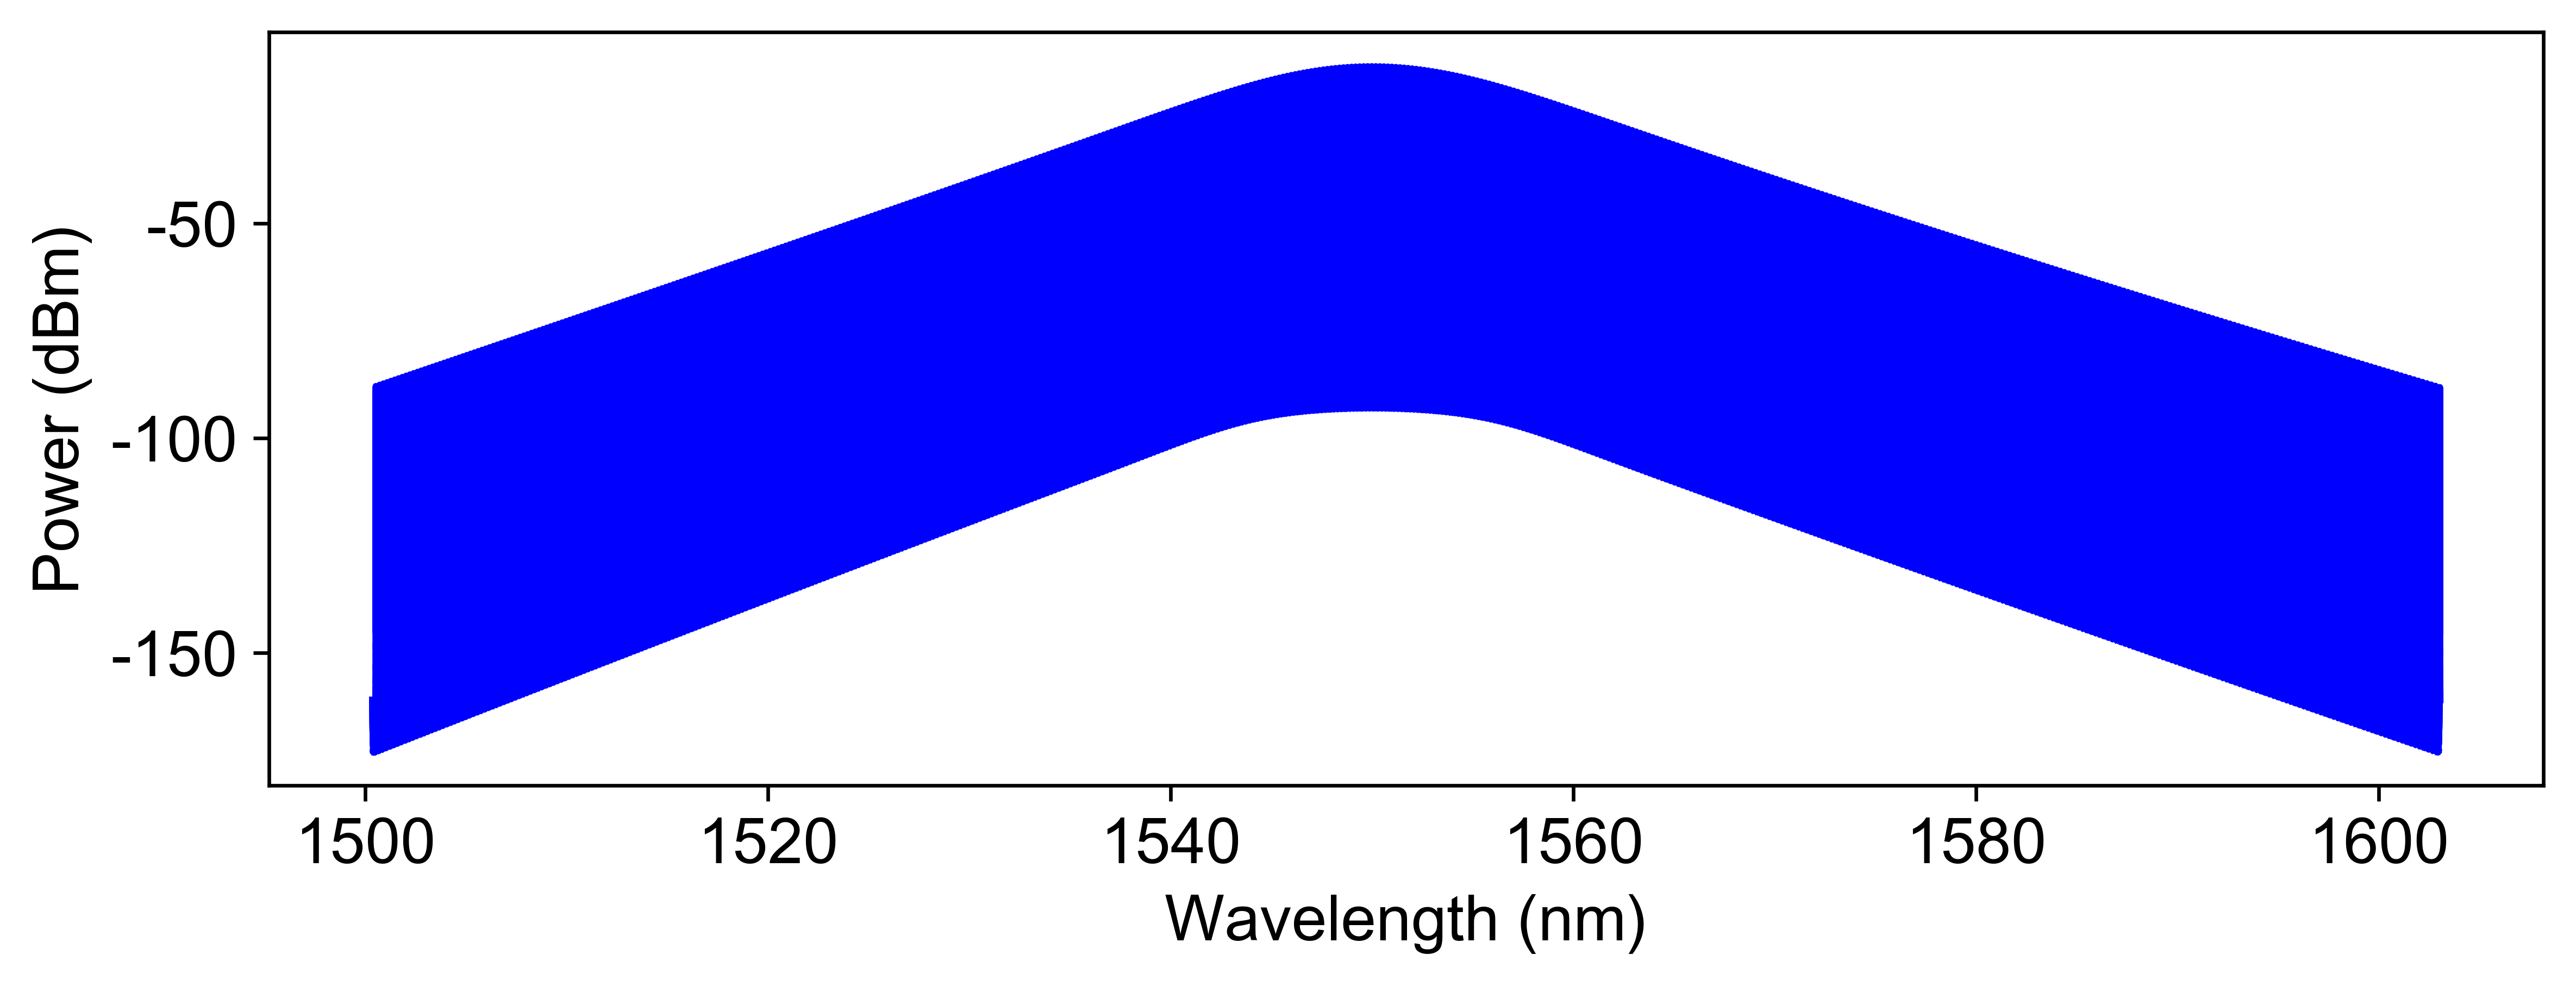
\includegraphics[width=0.48\linewidth]{figure/fig_18_0.png}
    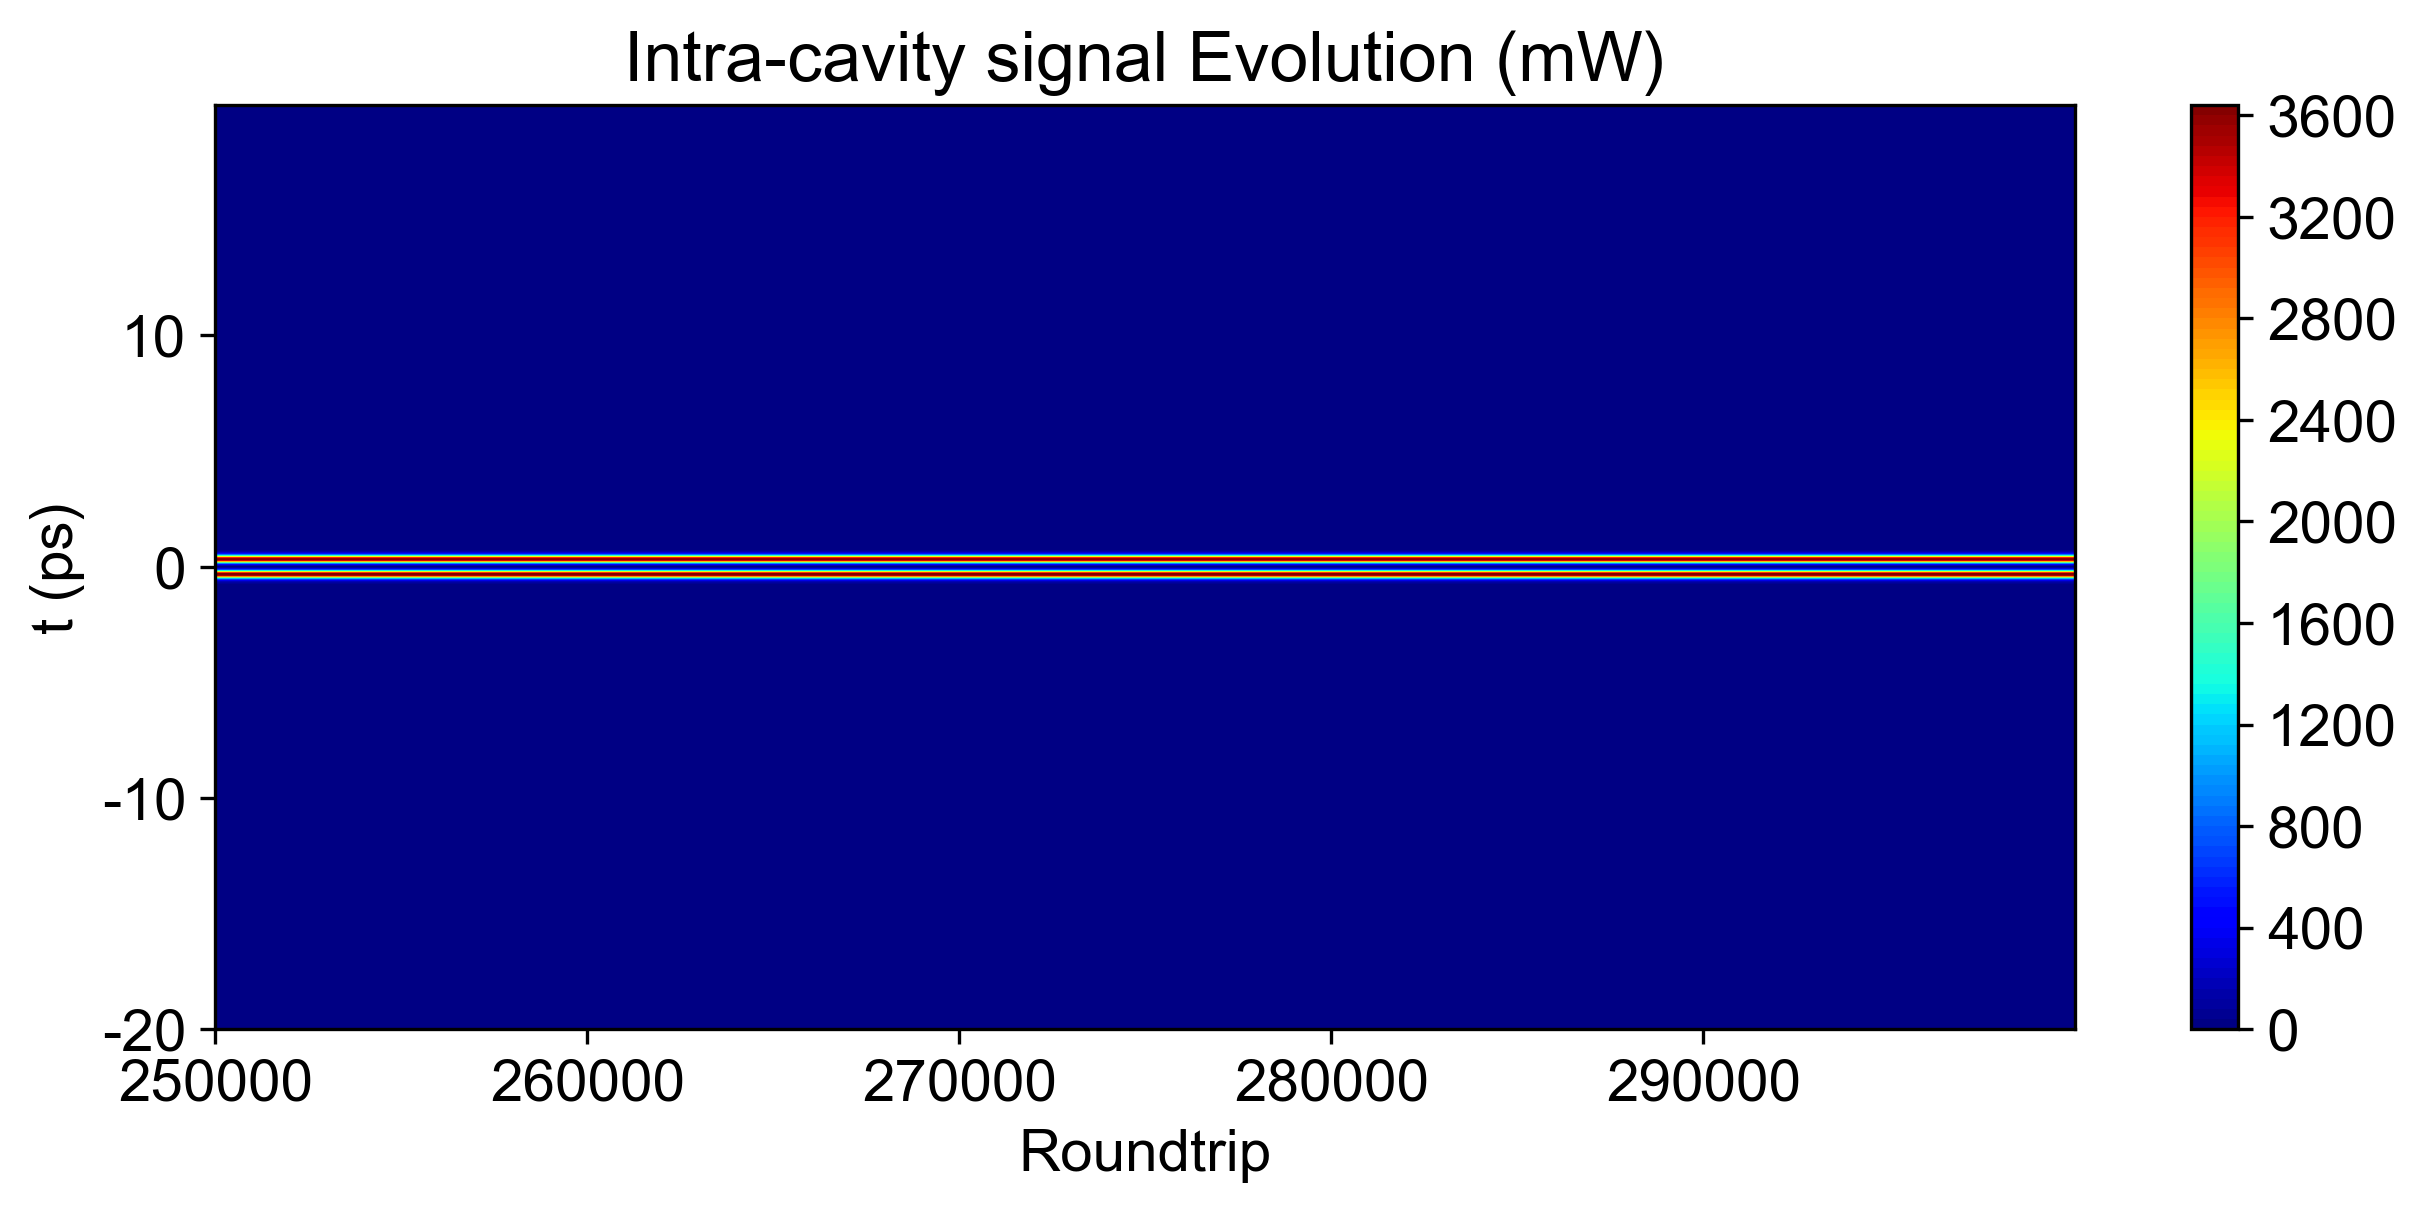
\includegraphics[width=0.48\linewidth]{figure/fig_19.png}
    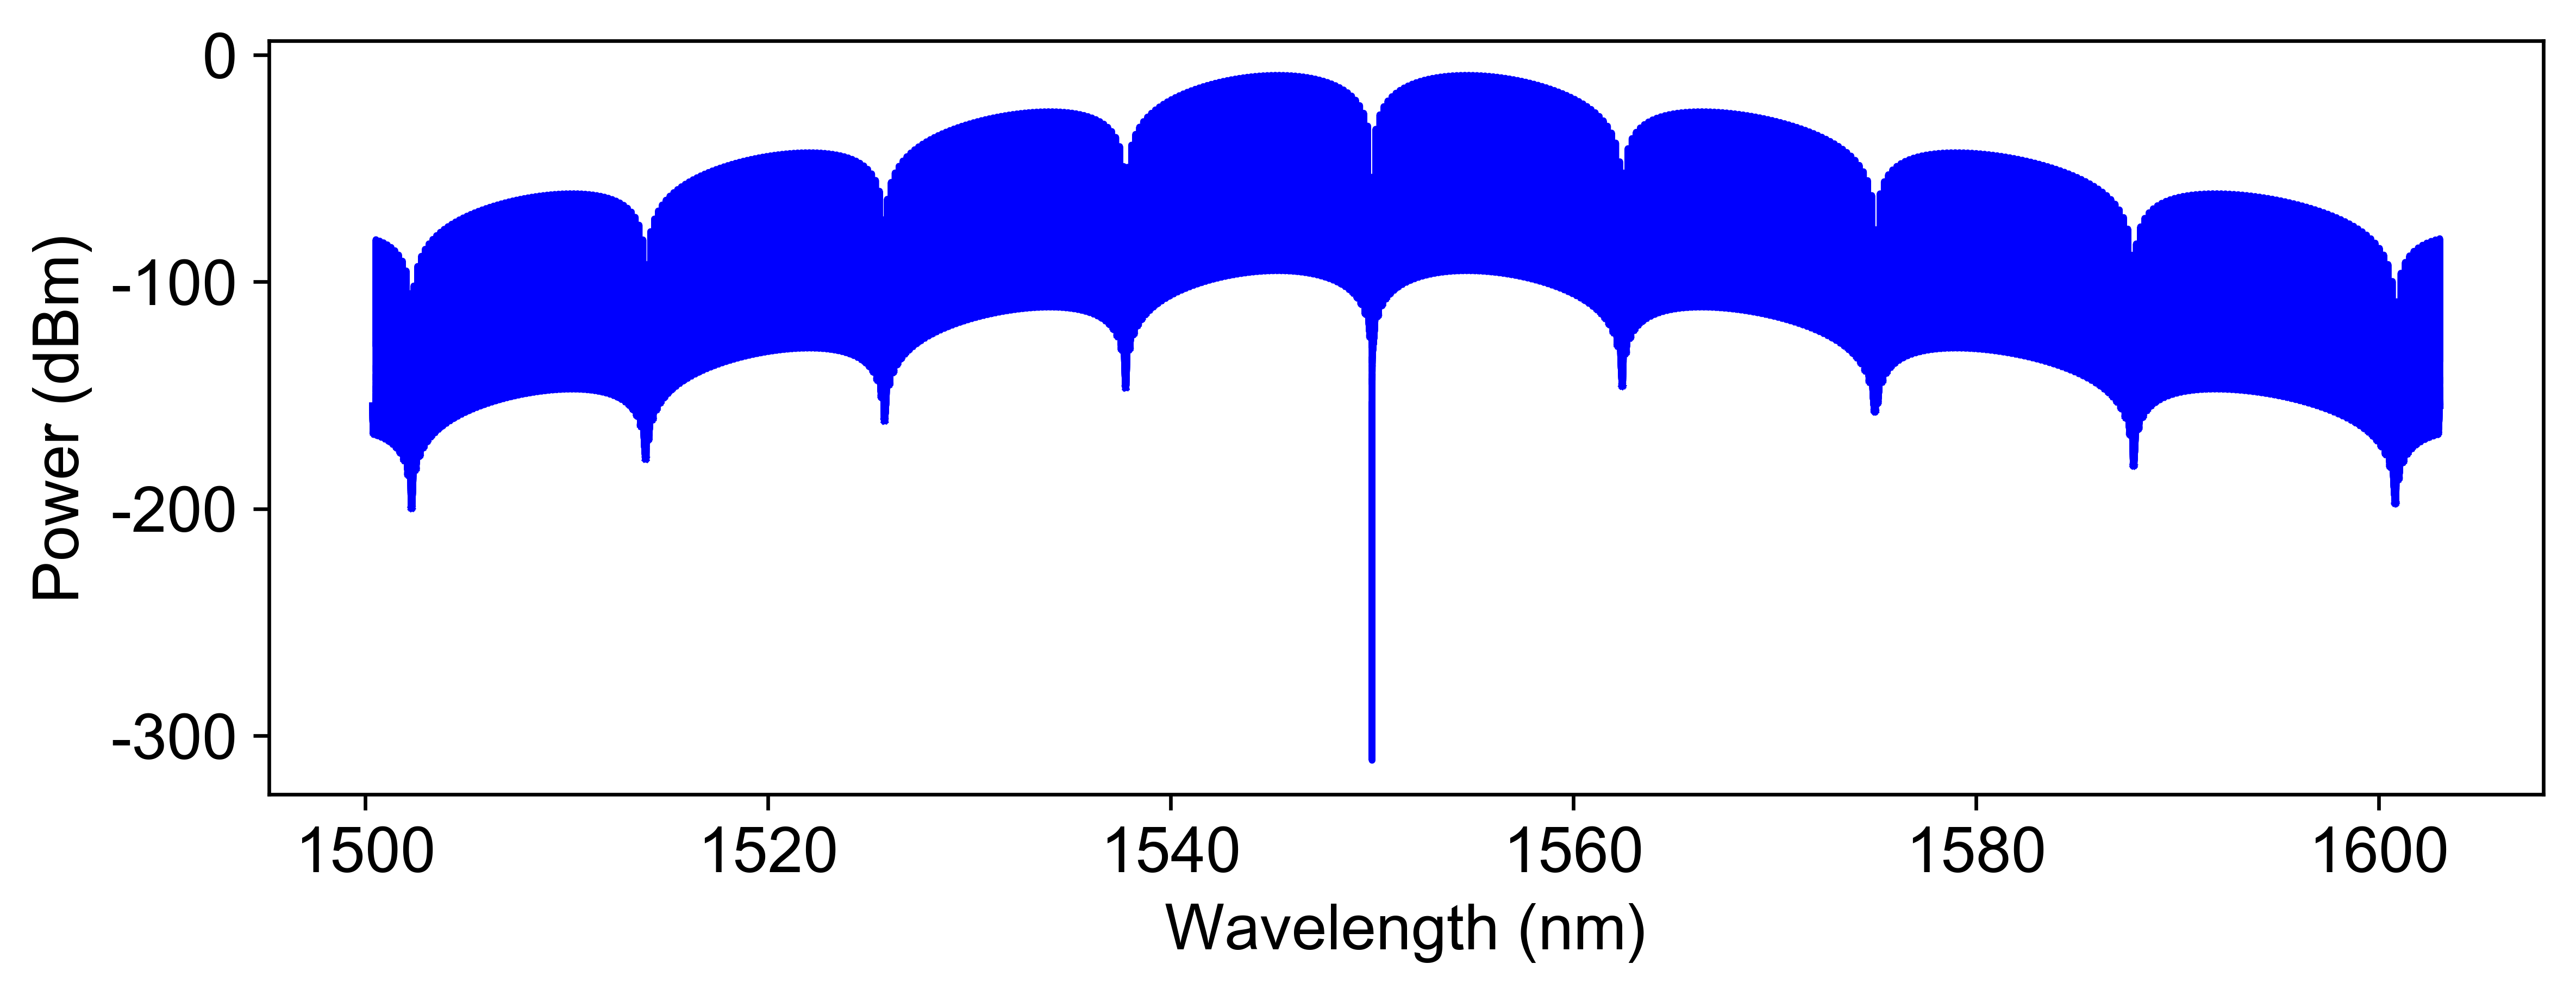
\includegraphics[width=0.48\linewidth]{figure/fig_19_0.png}
    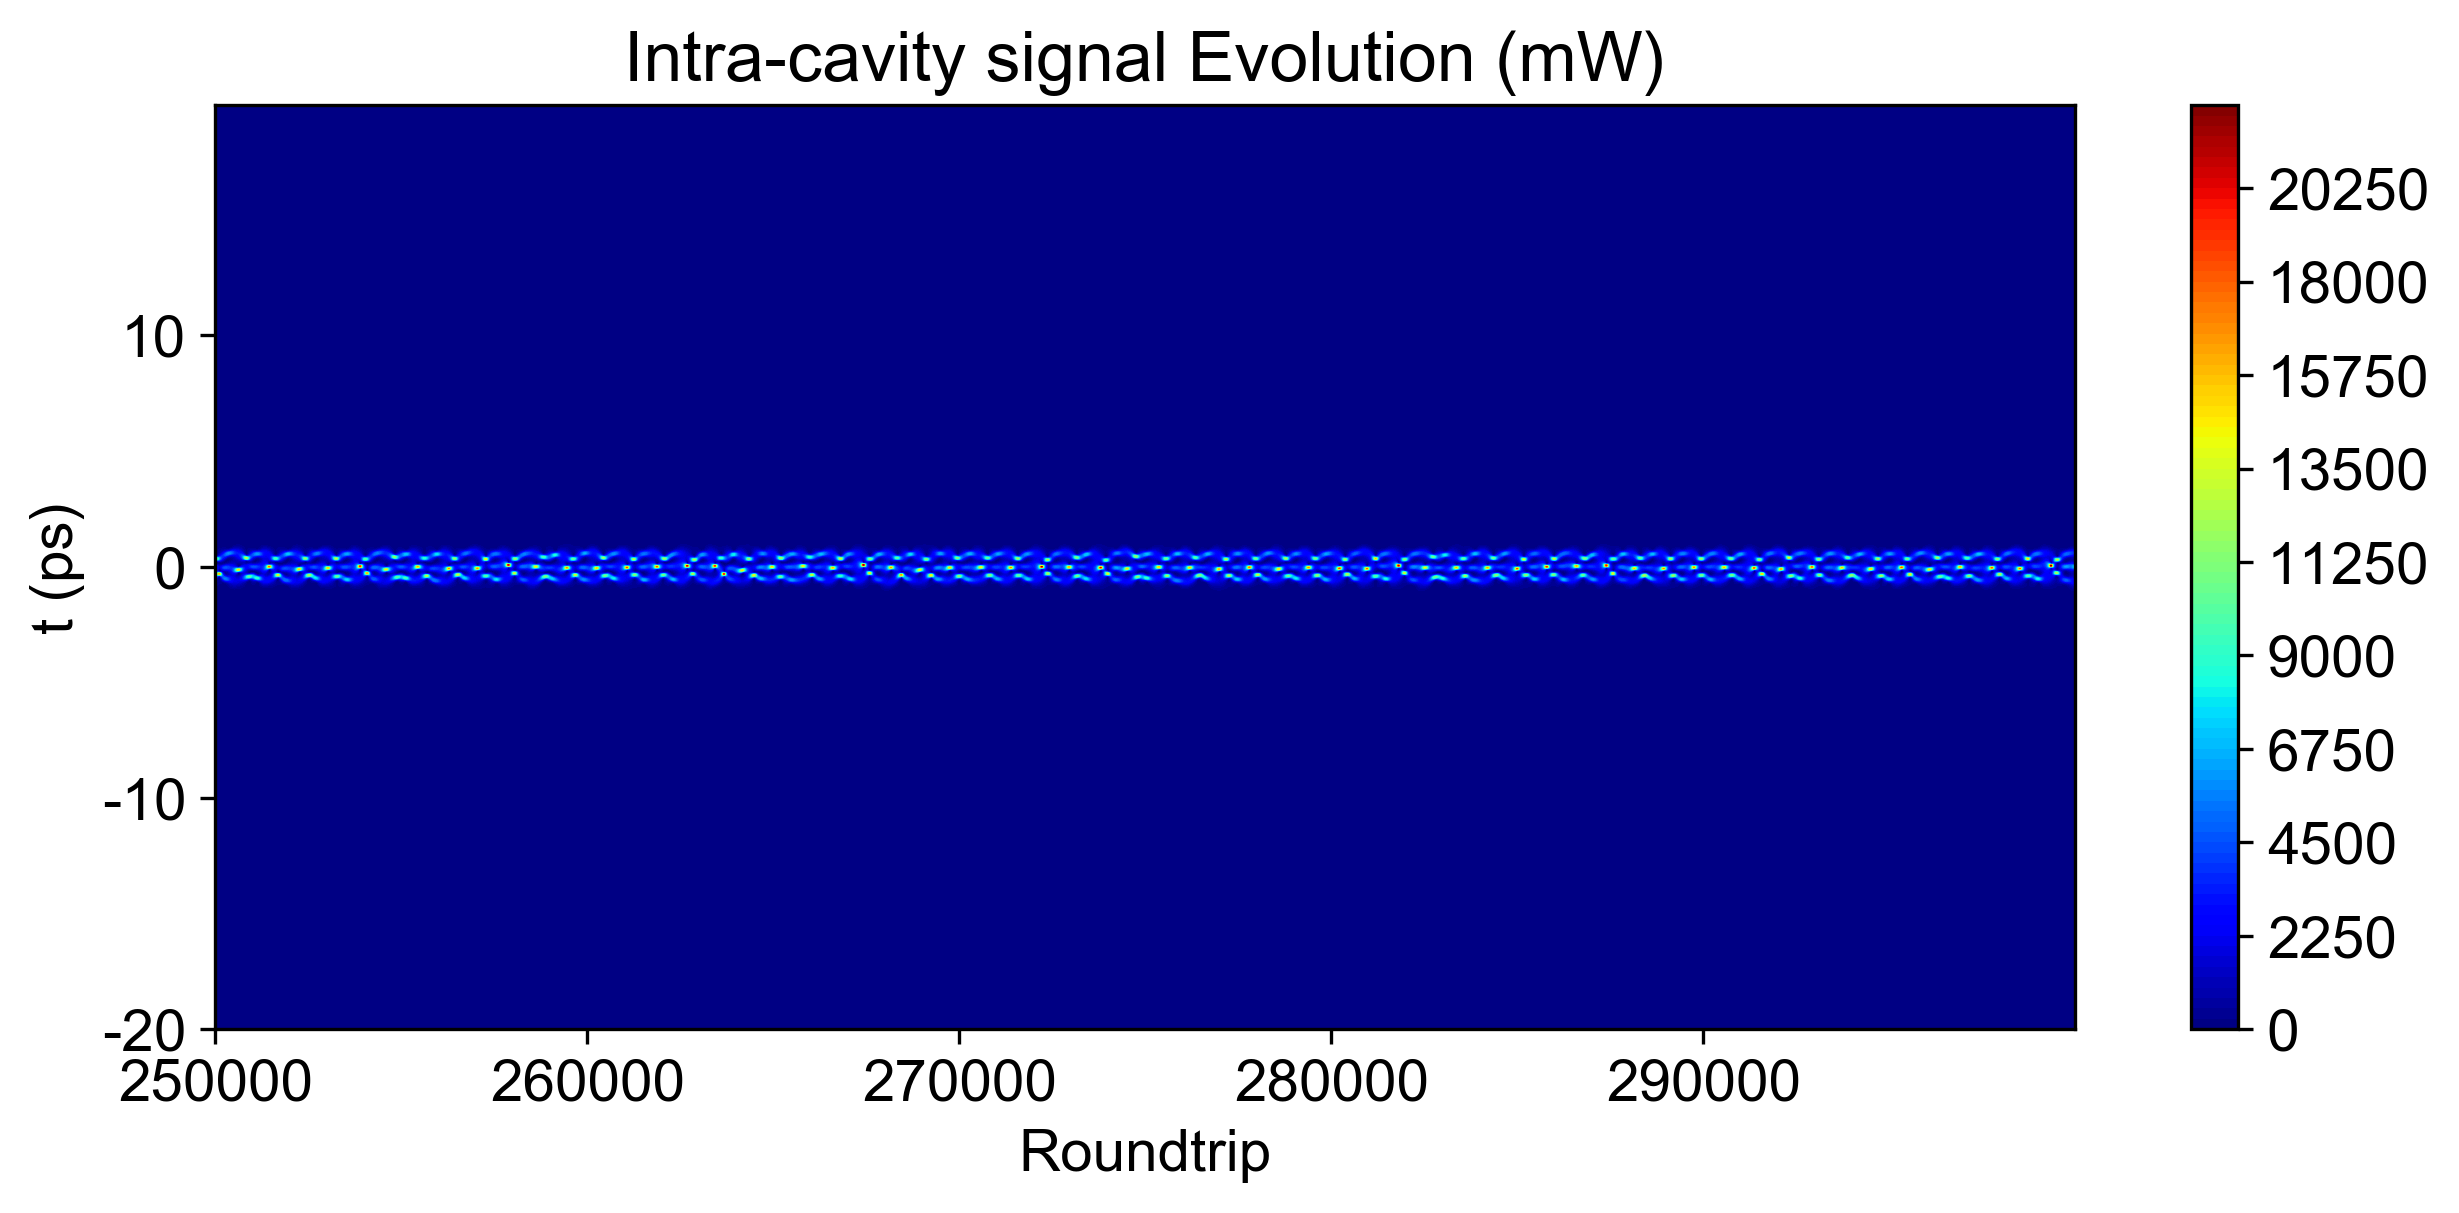
\includegraphics[width=0.48\linewidth]{figure/fig_20.png}
    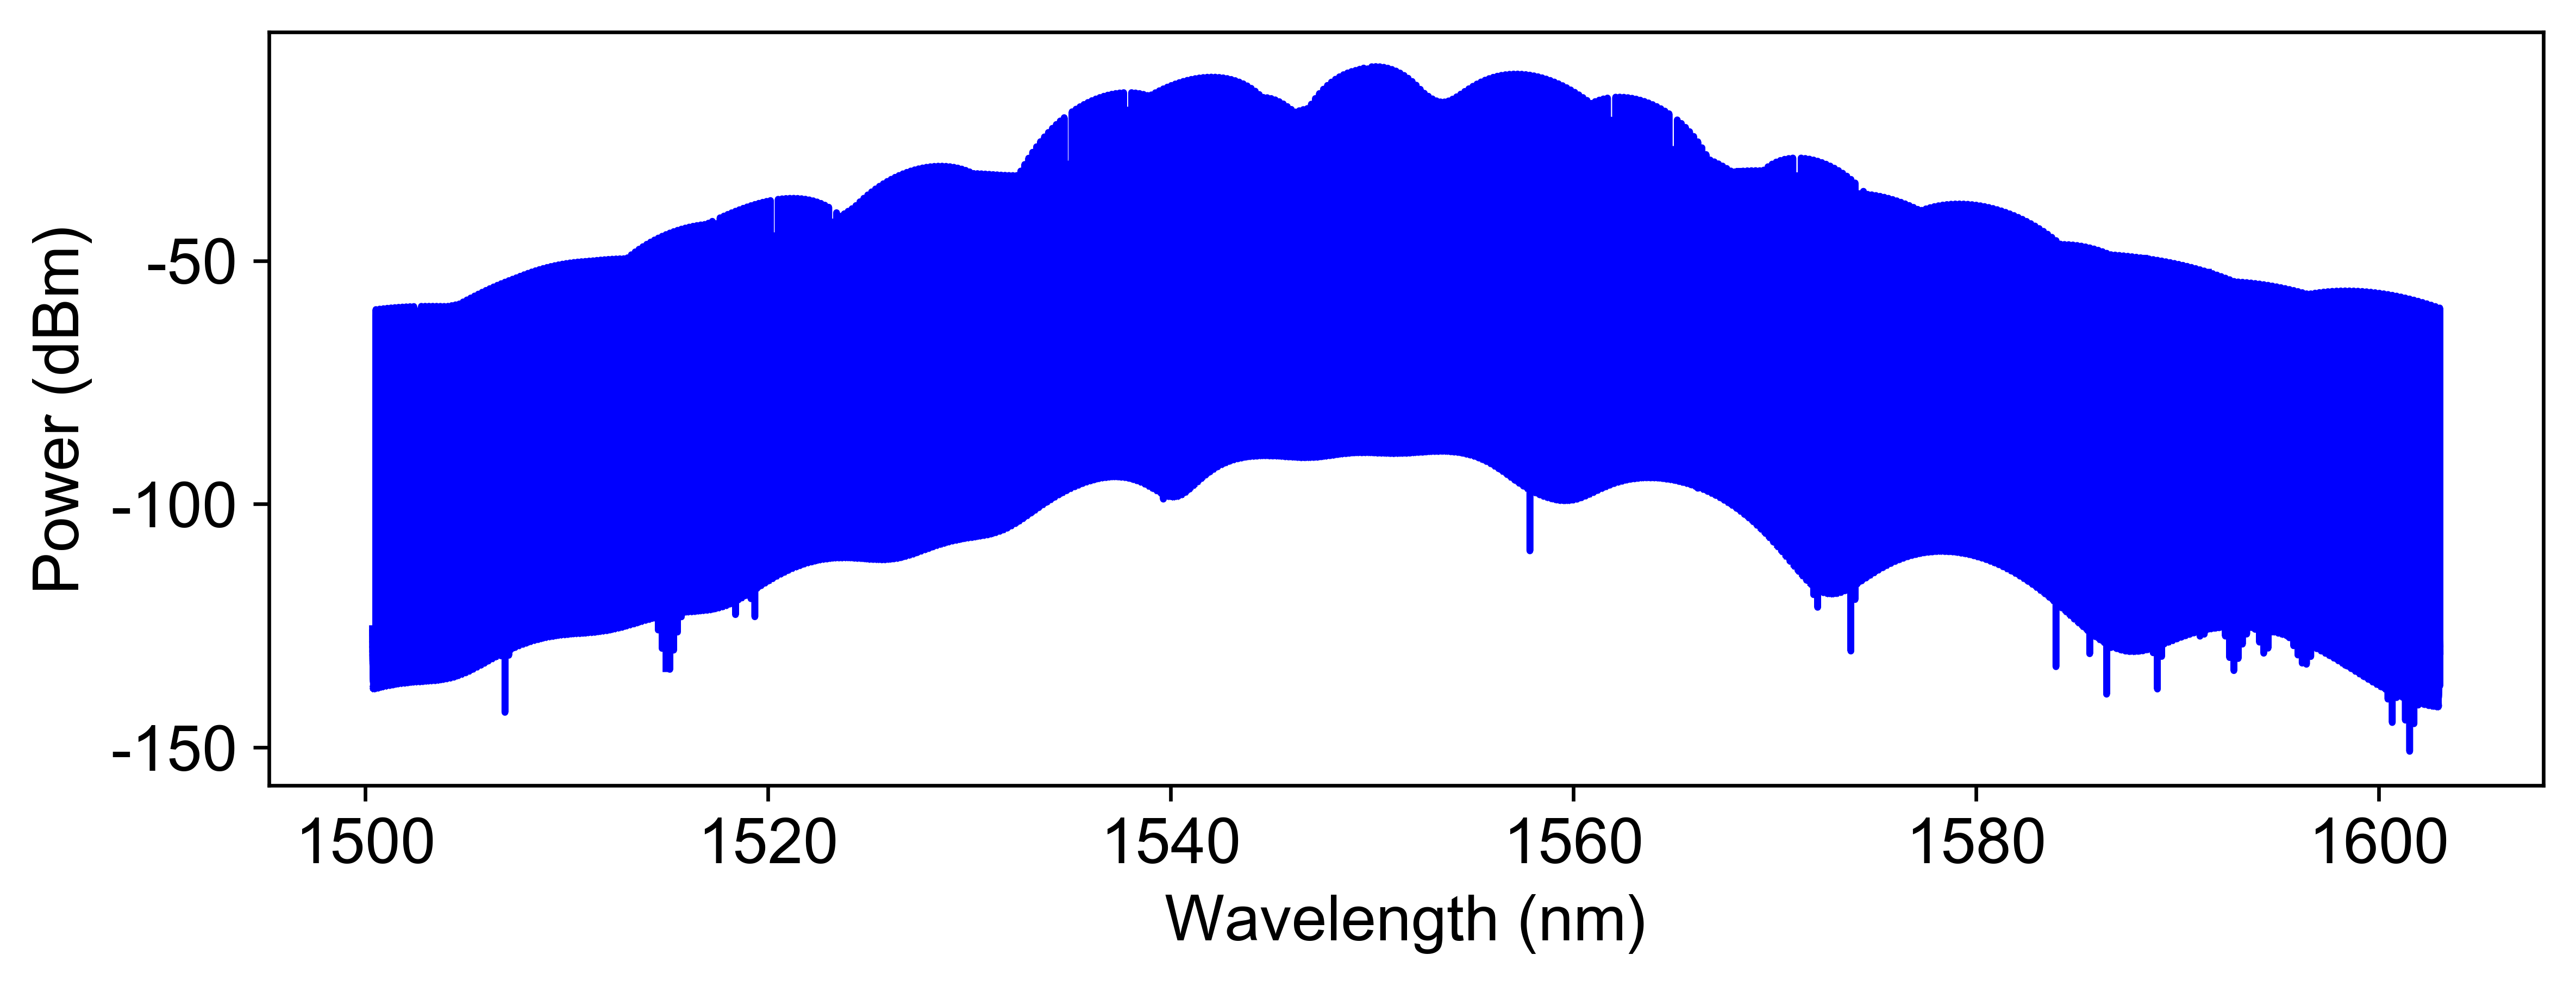
\includegraphics[width=0.48\linewidth]{figure/fig_20_0.png}
    \caption{左列:腔内信号光场的稳态,对应的光谱。从上到下泵浦功率依次为:20,50,100,200毫瓦。}
    \label{fig:enter-label}
\end{figure}
泵浦功率越小,越接近锁模态。
\subsection{重频}
以调制深度$M = 0.5$,泵浦功率$P_{in} = 100mW$,改变$FSR$进行仿真。\\
\begin{figure}[htbp]
    \centering
    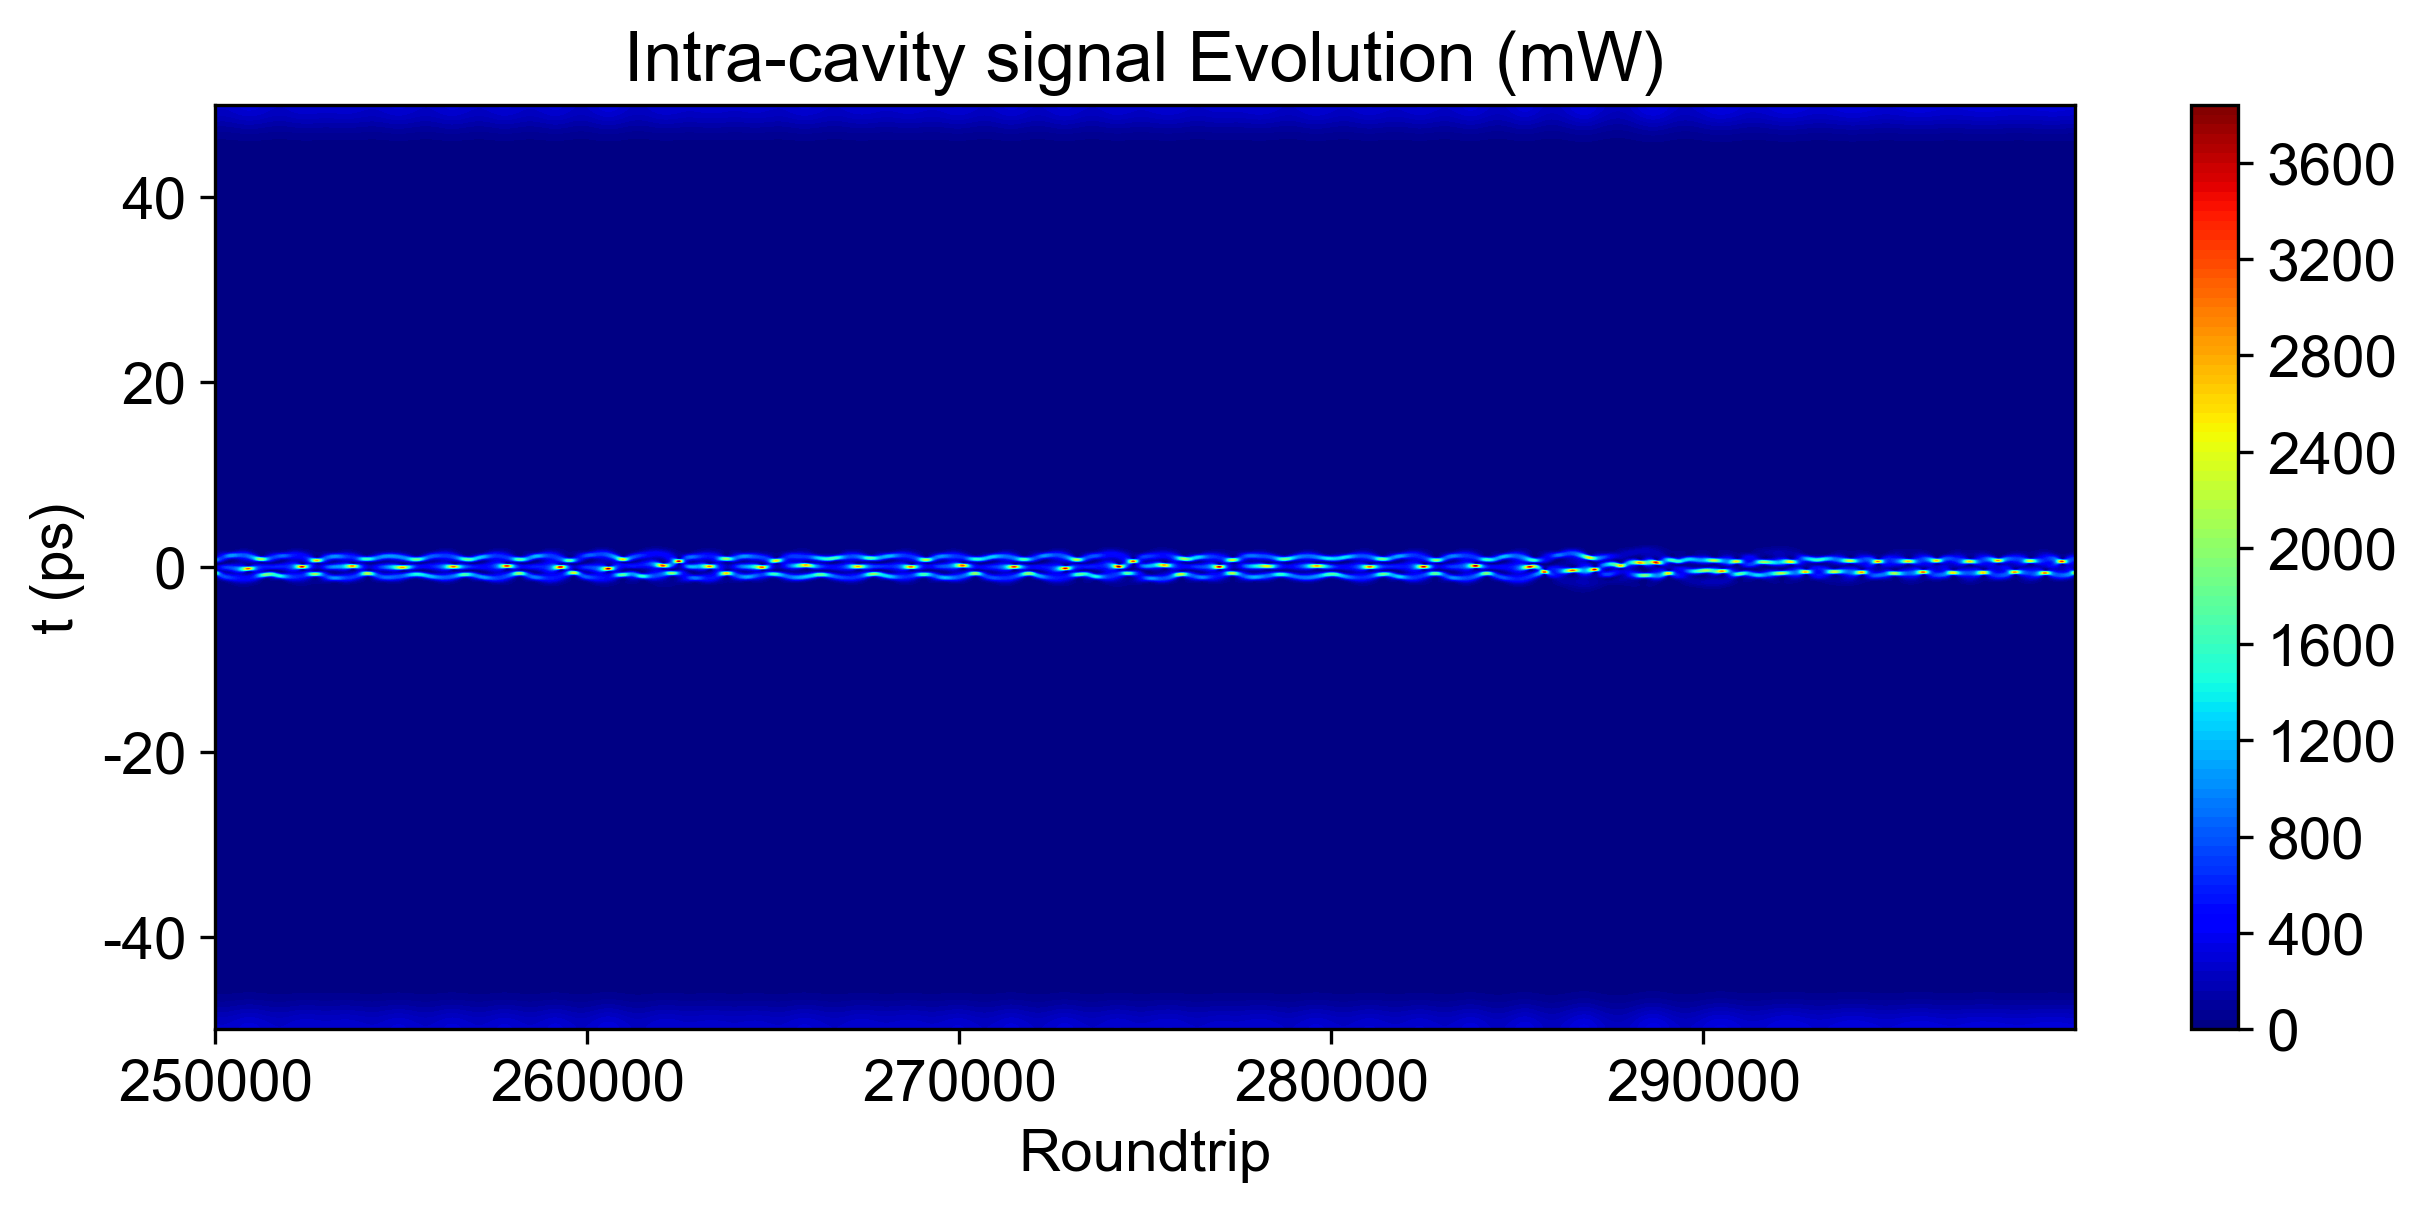
\includegraphics[width=0.48\linewidth]{figure/fig_21.png}
    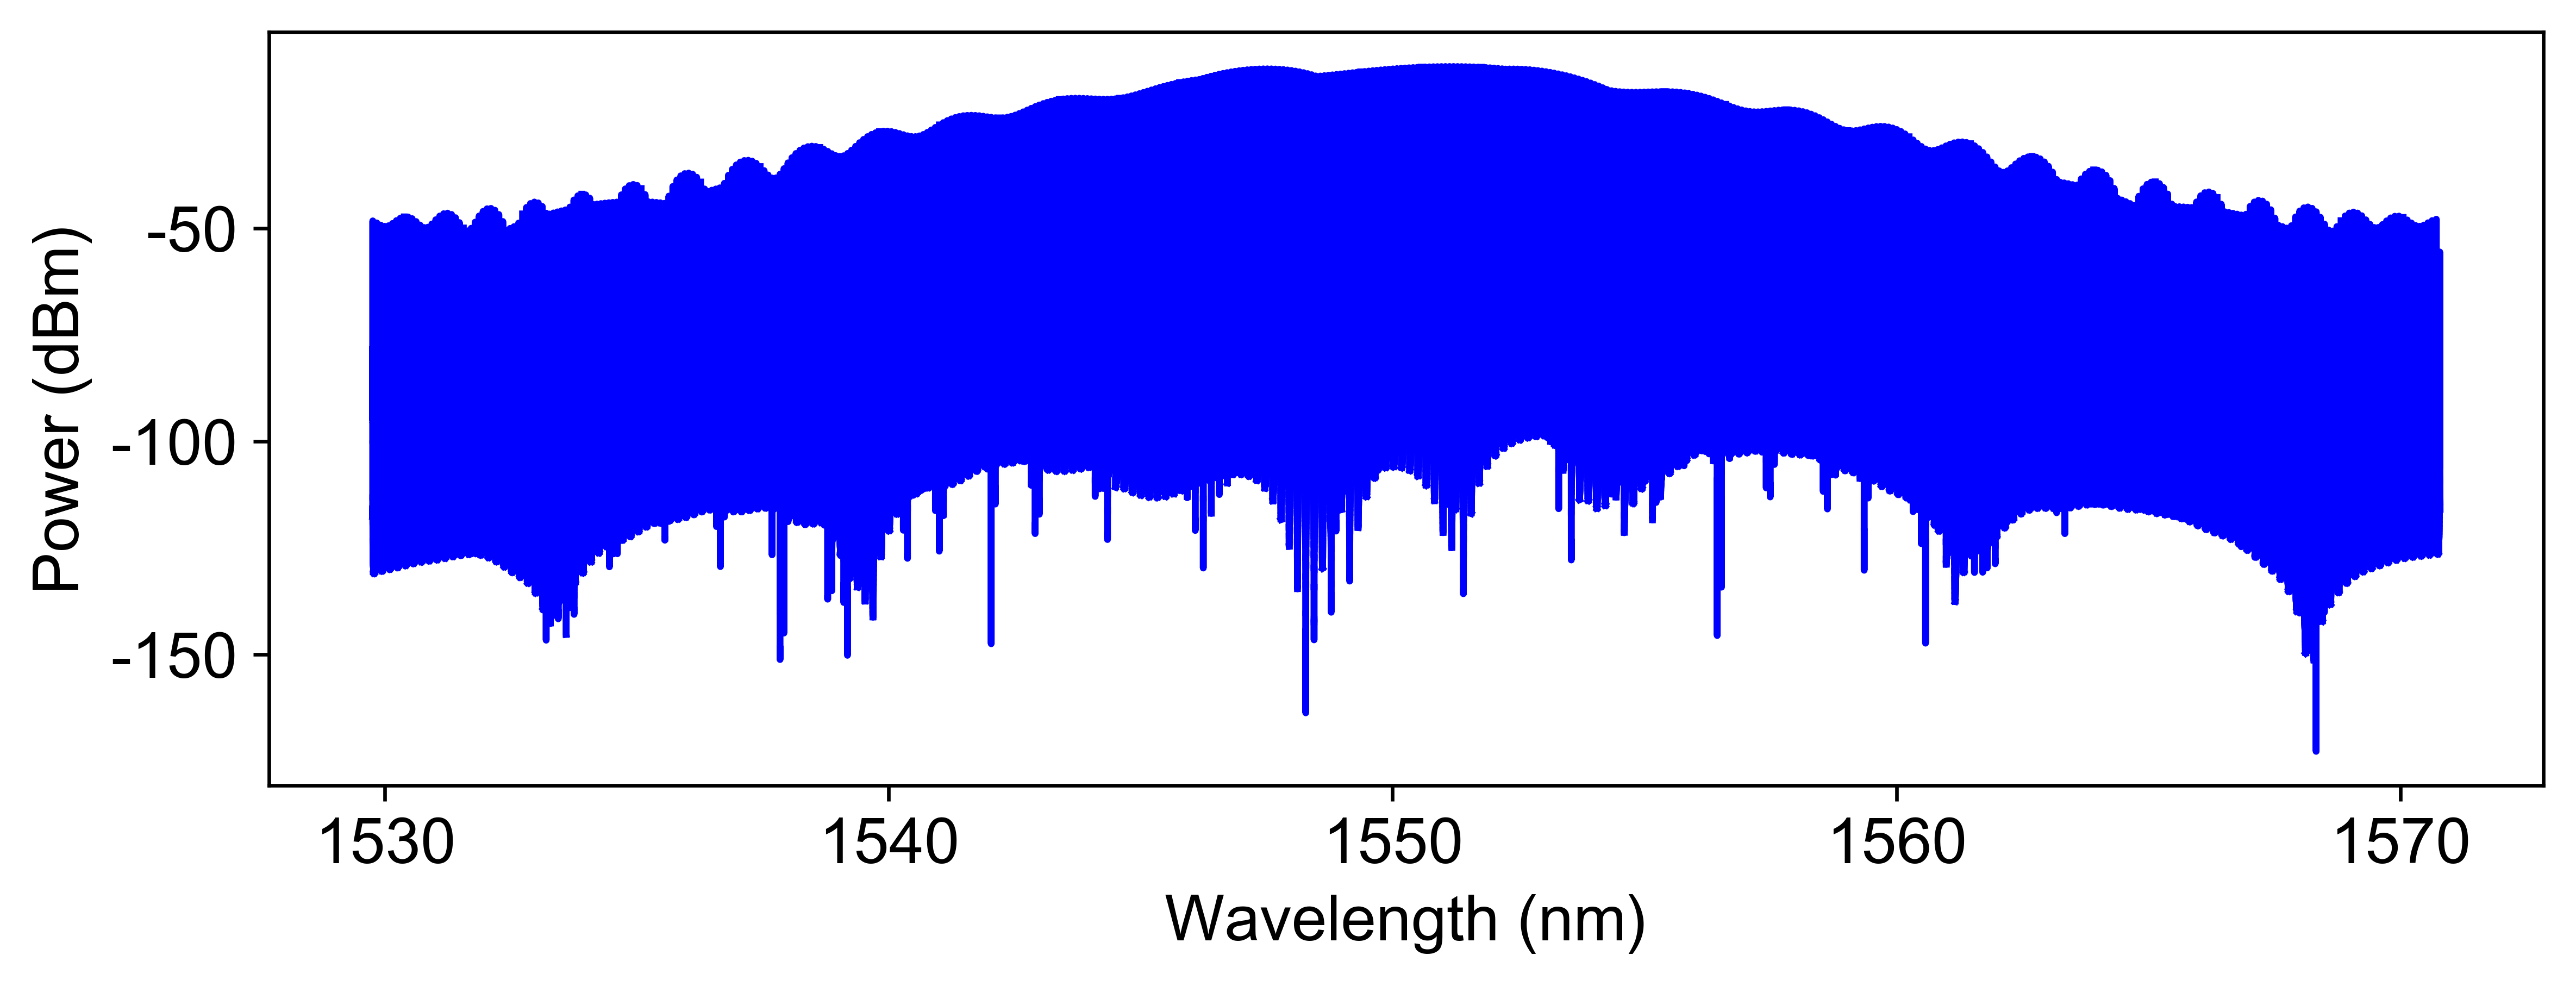
\includegraphics[width=0.48\linewidth]{figure/fig_21_0.png}
    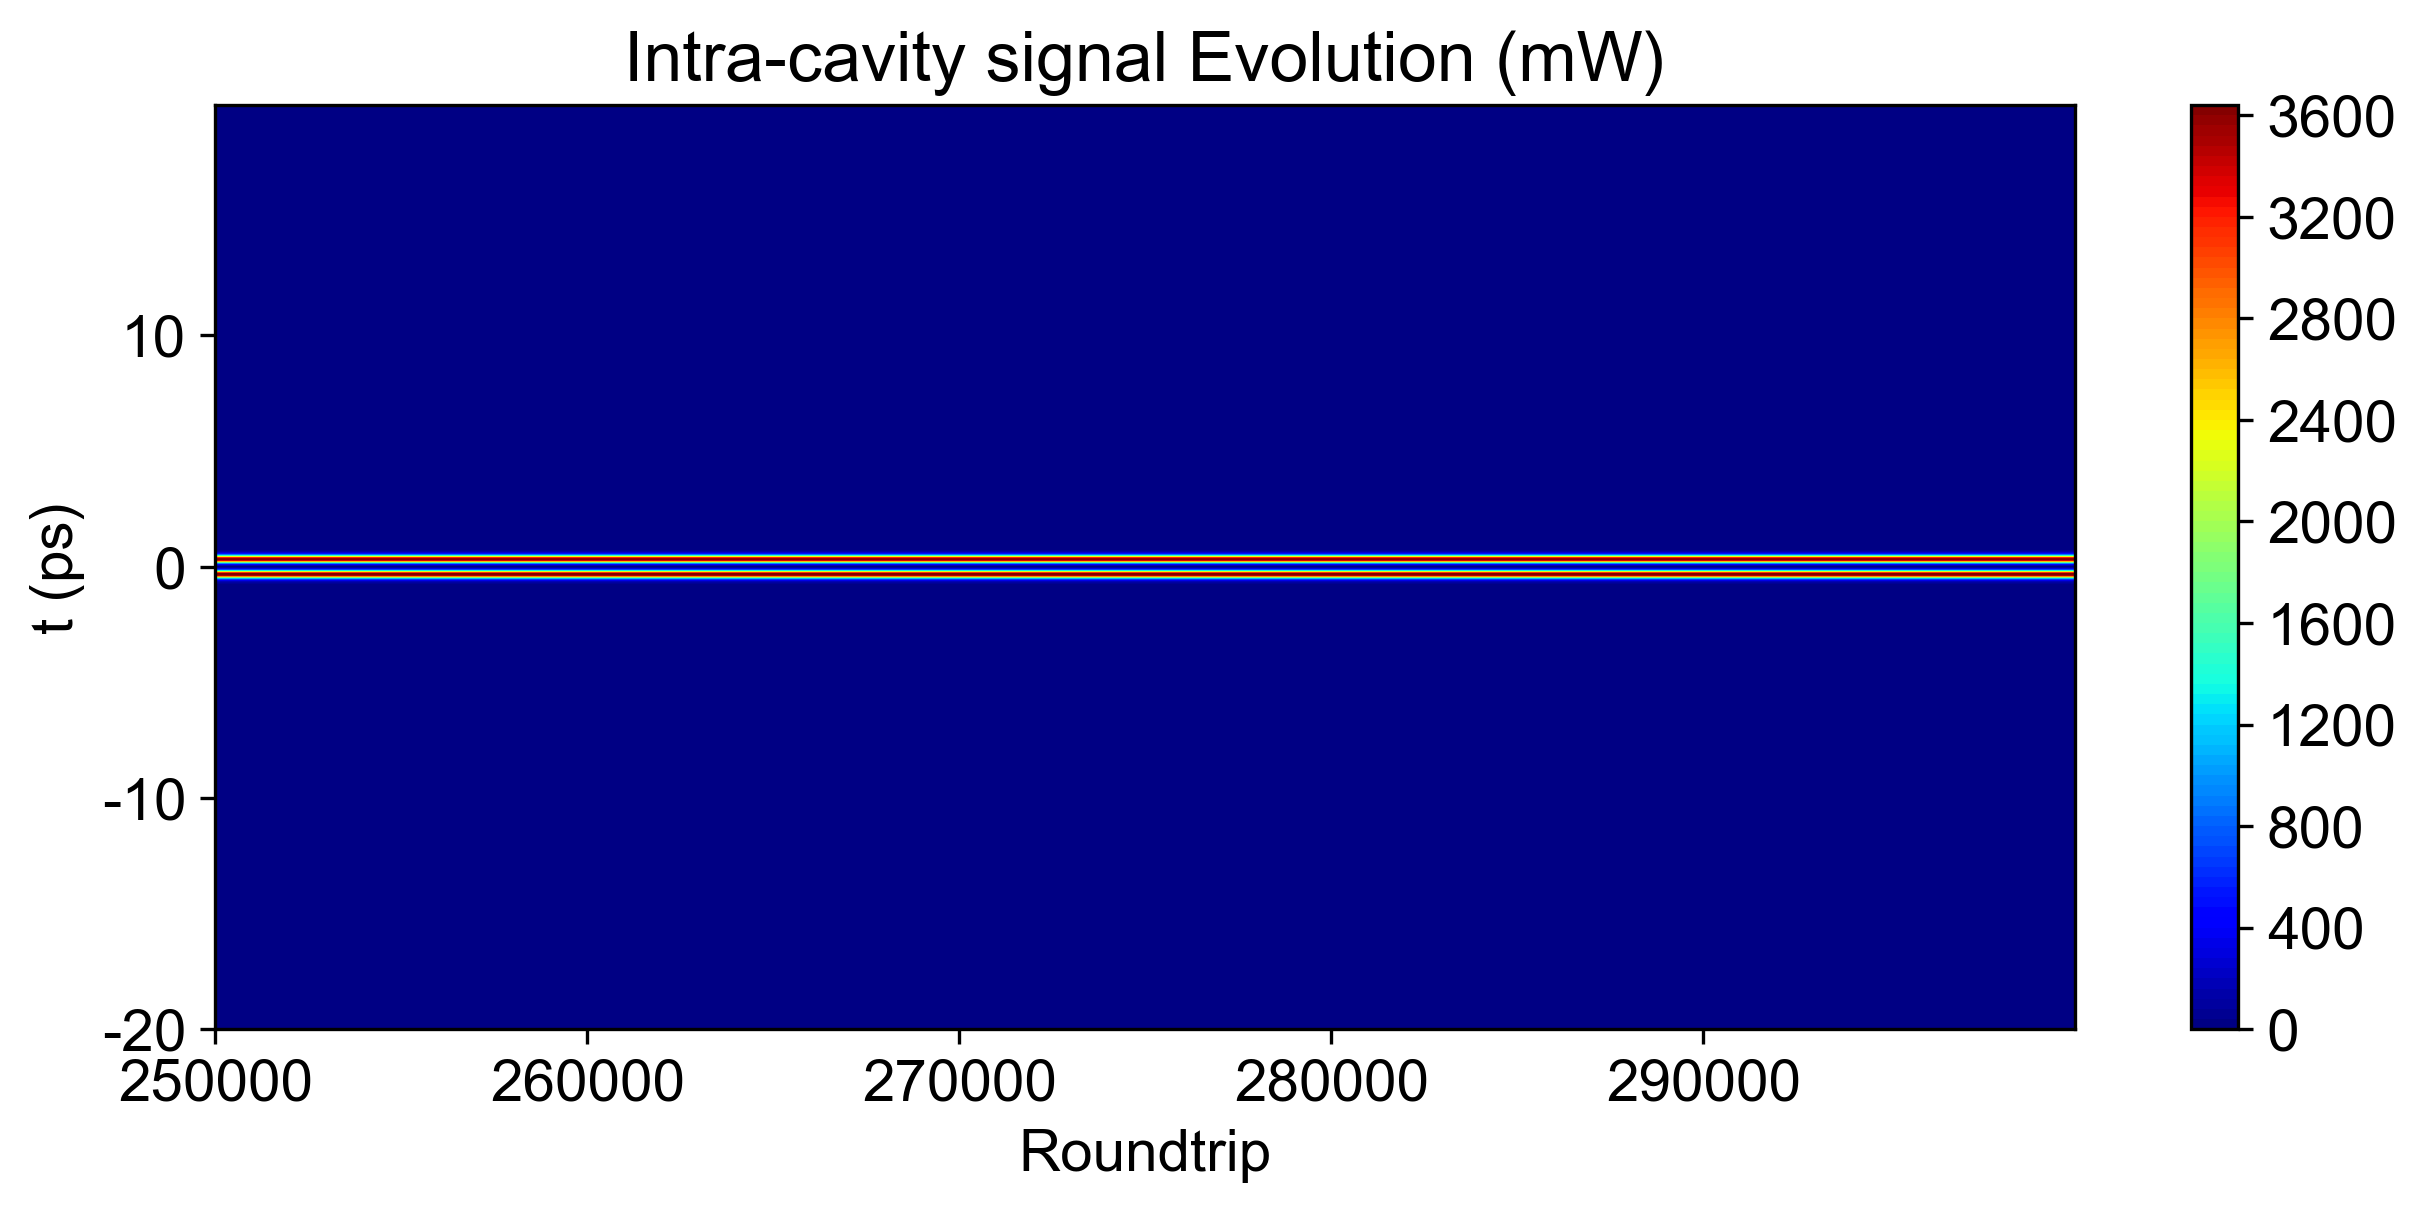
\includegraphics[width=0.48\linewidth]{figure/fig_22.png}
    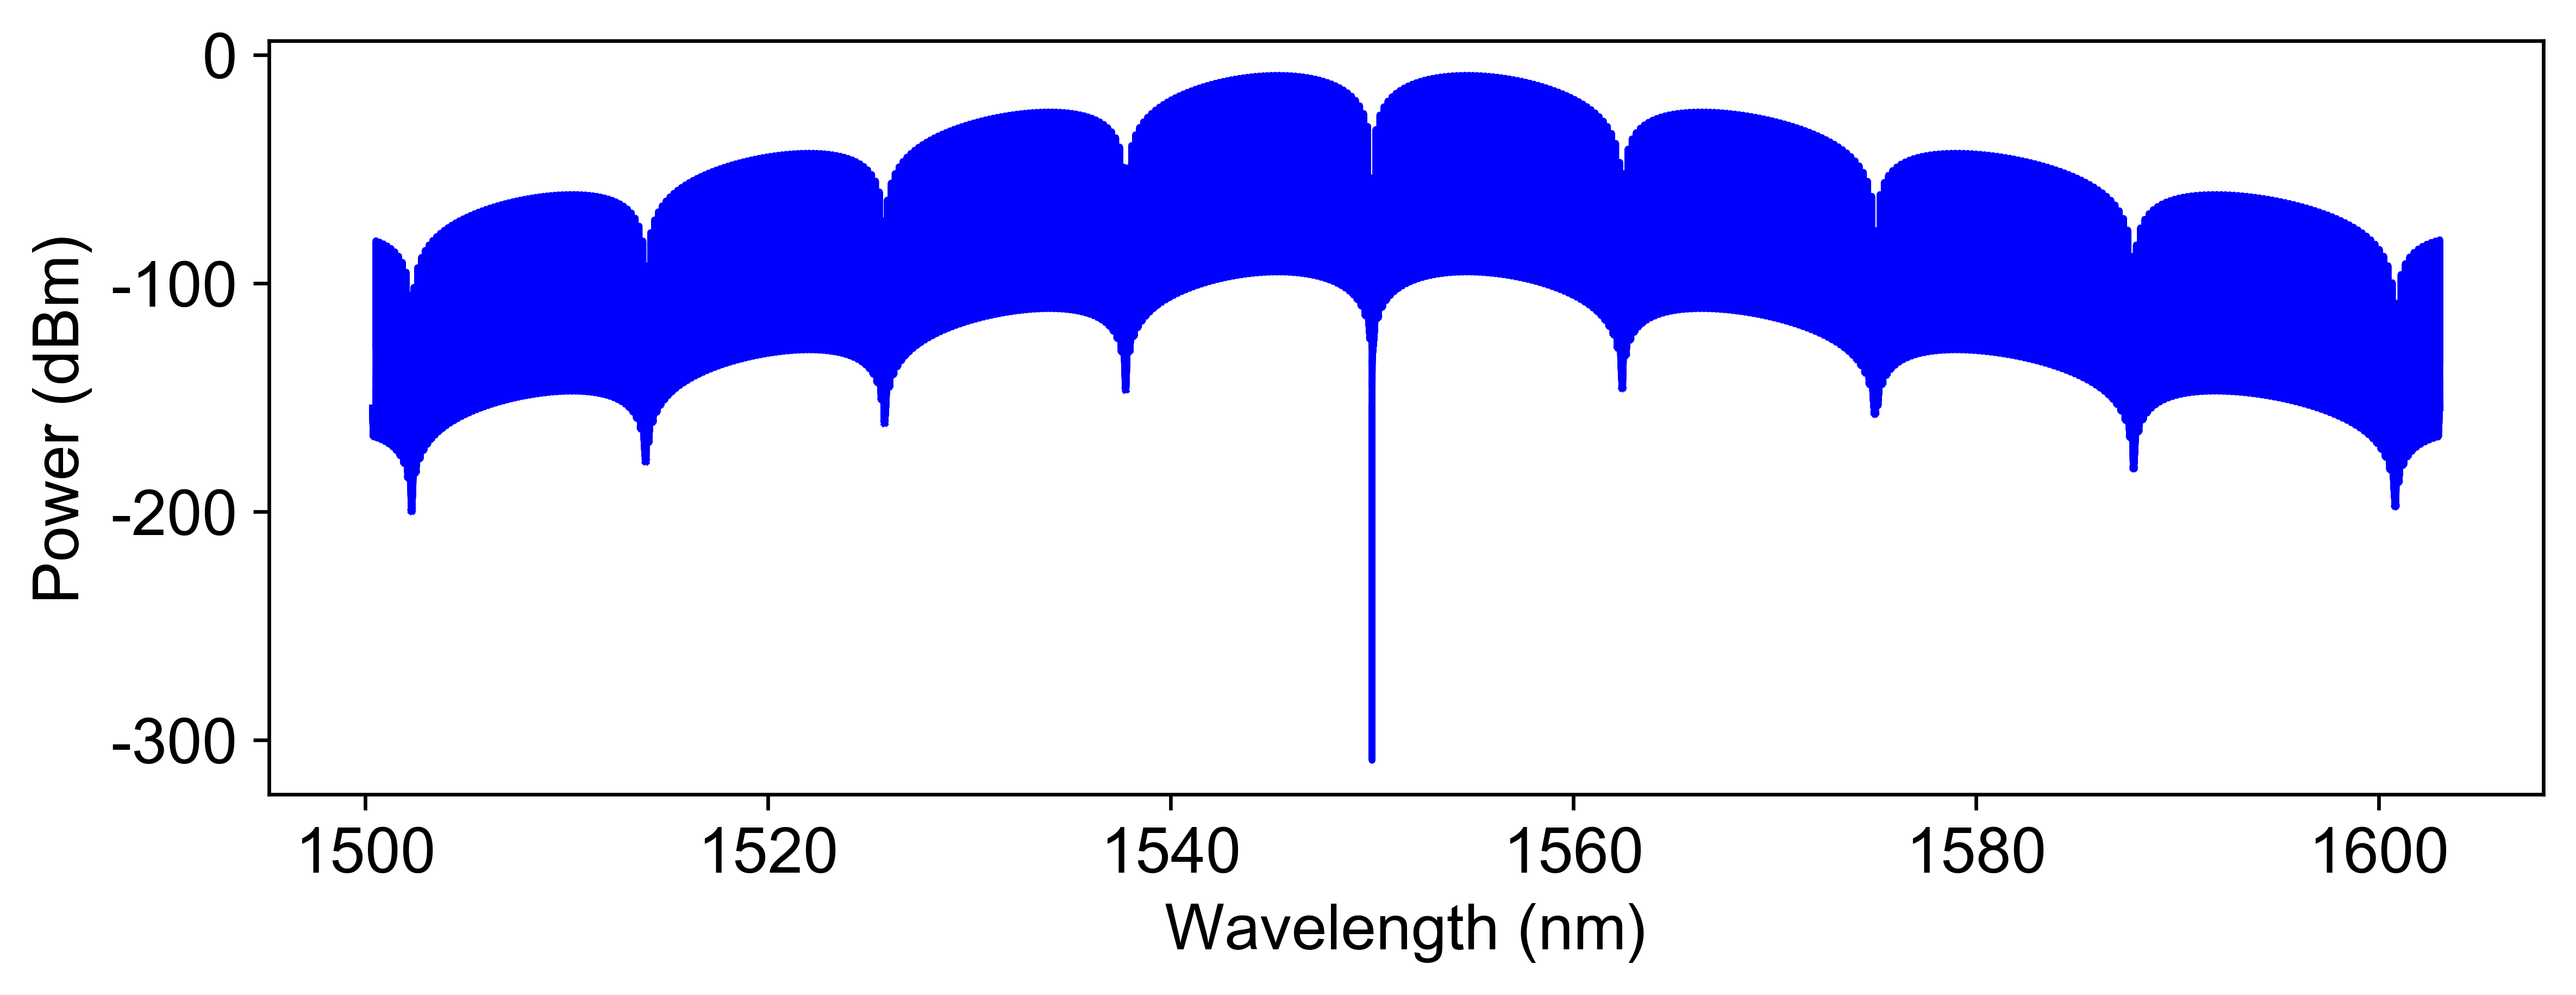
\includegraphics[width=0.48\linewidth]{figure/fig_22_0.png}
    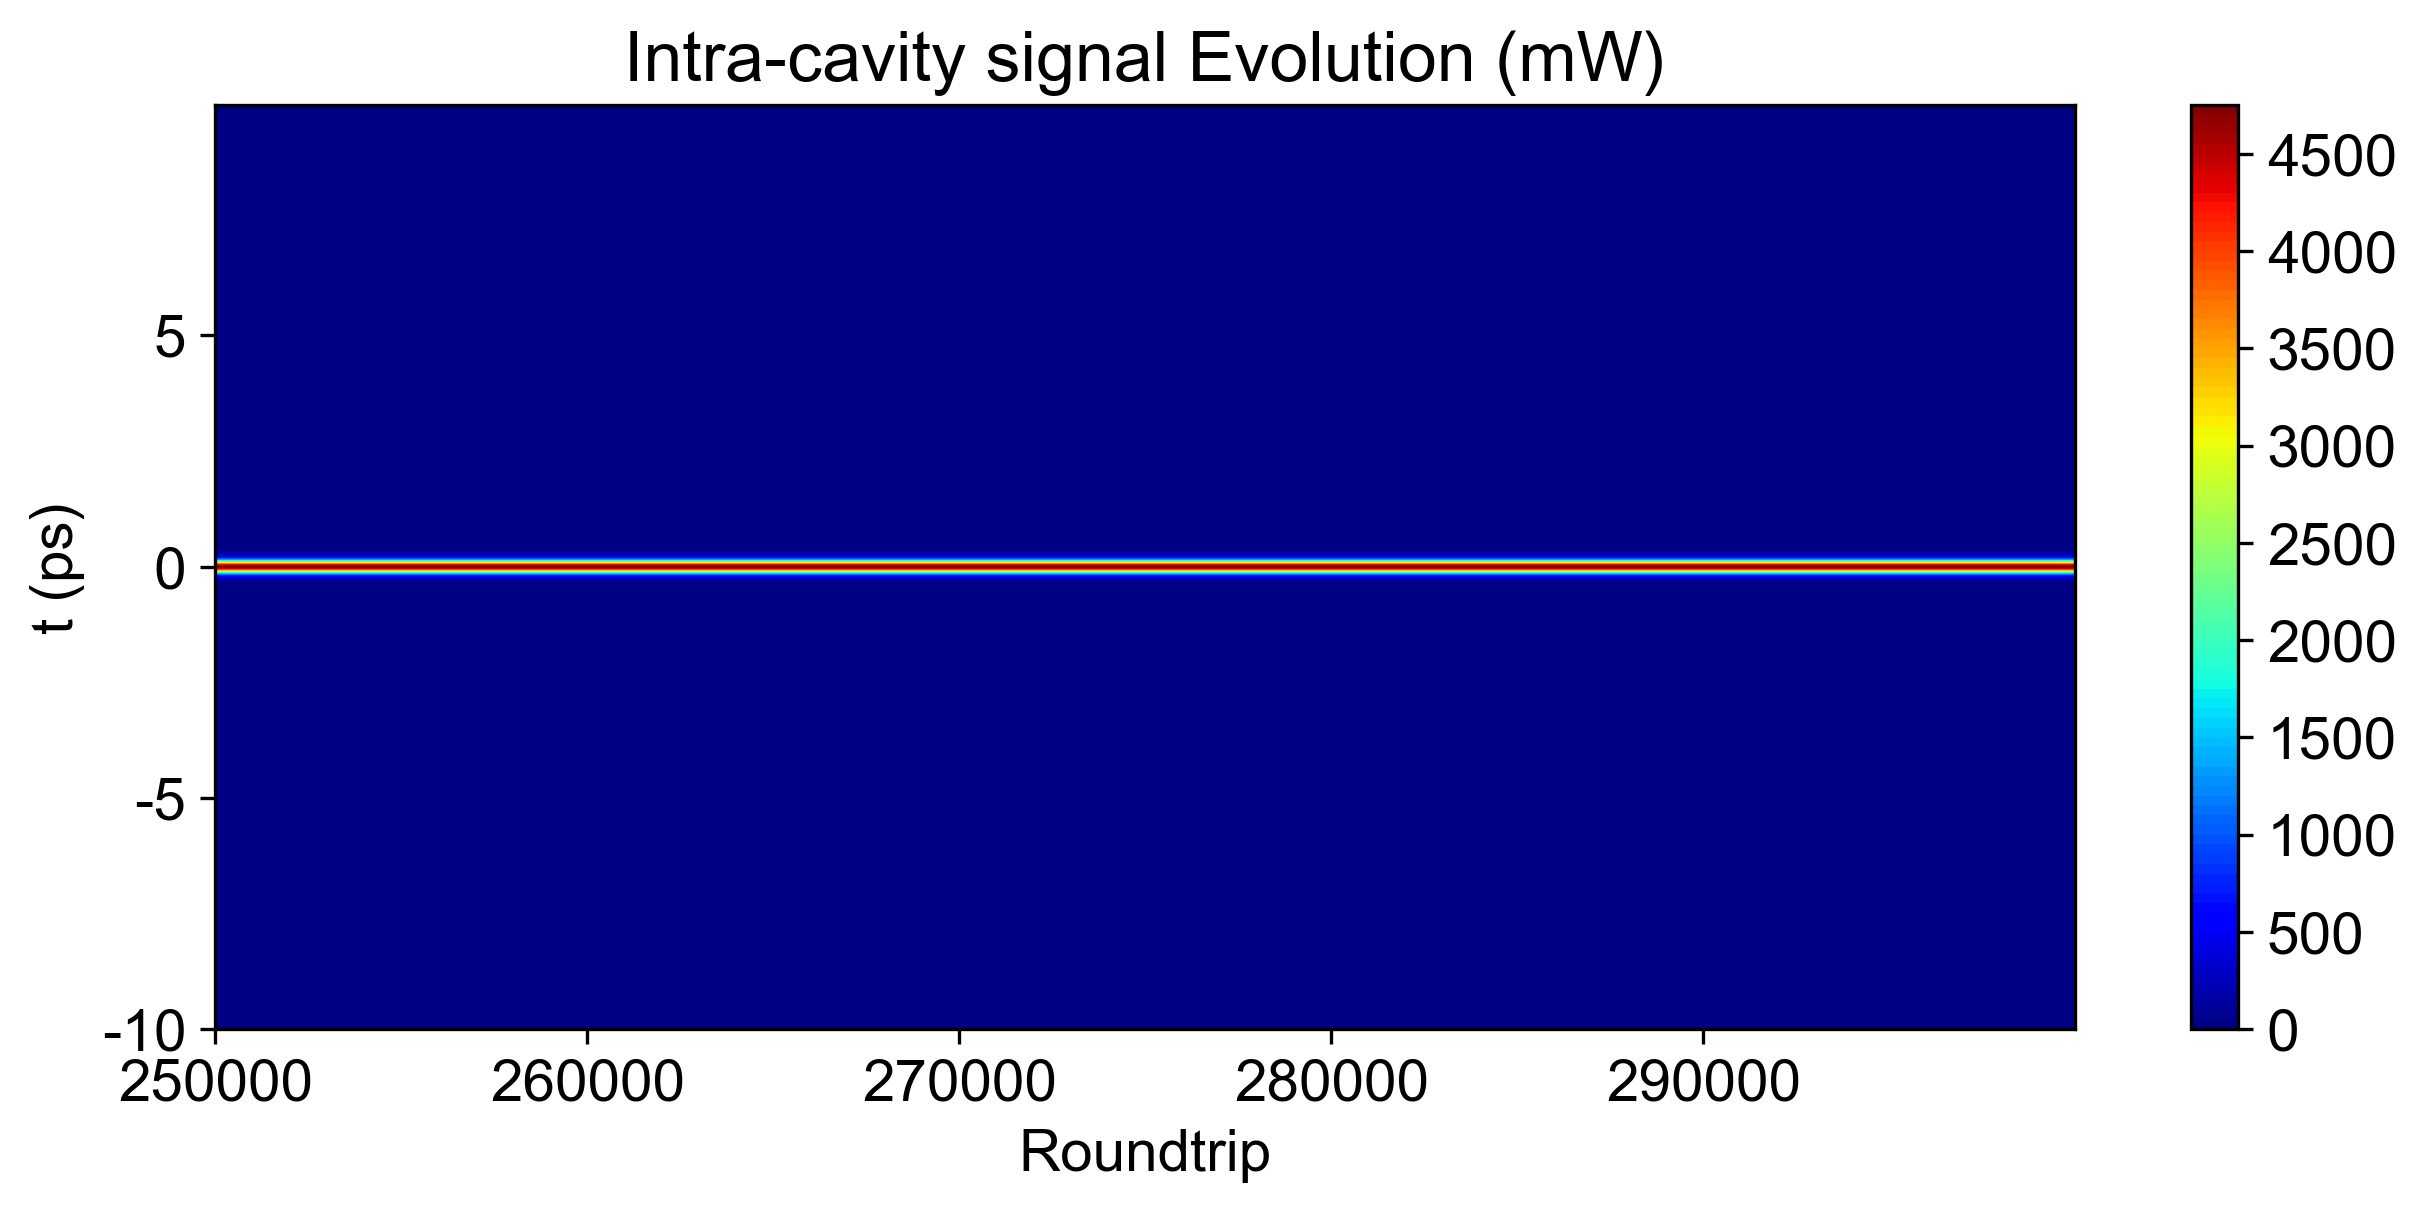
\includegraphics[width=0.48\linewidth]{figure/fig_23.png}
    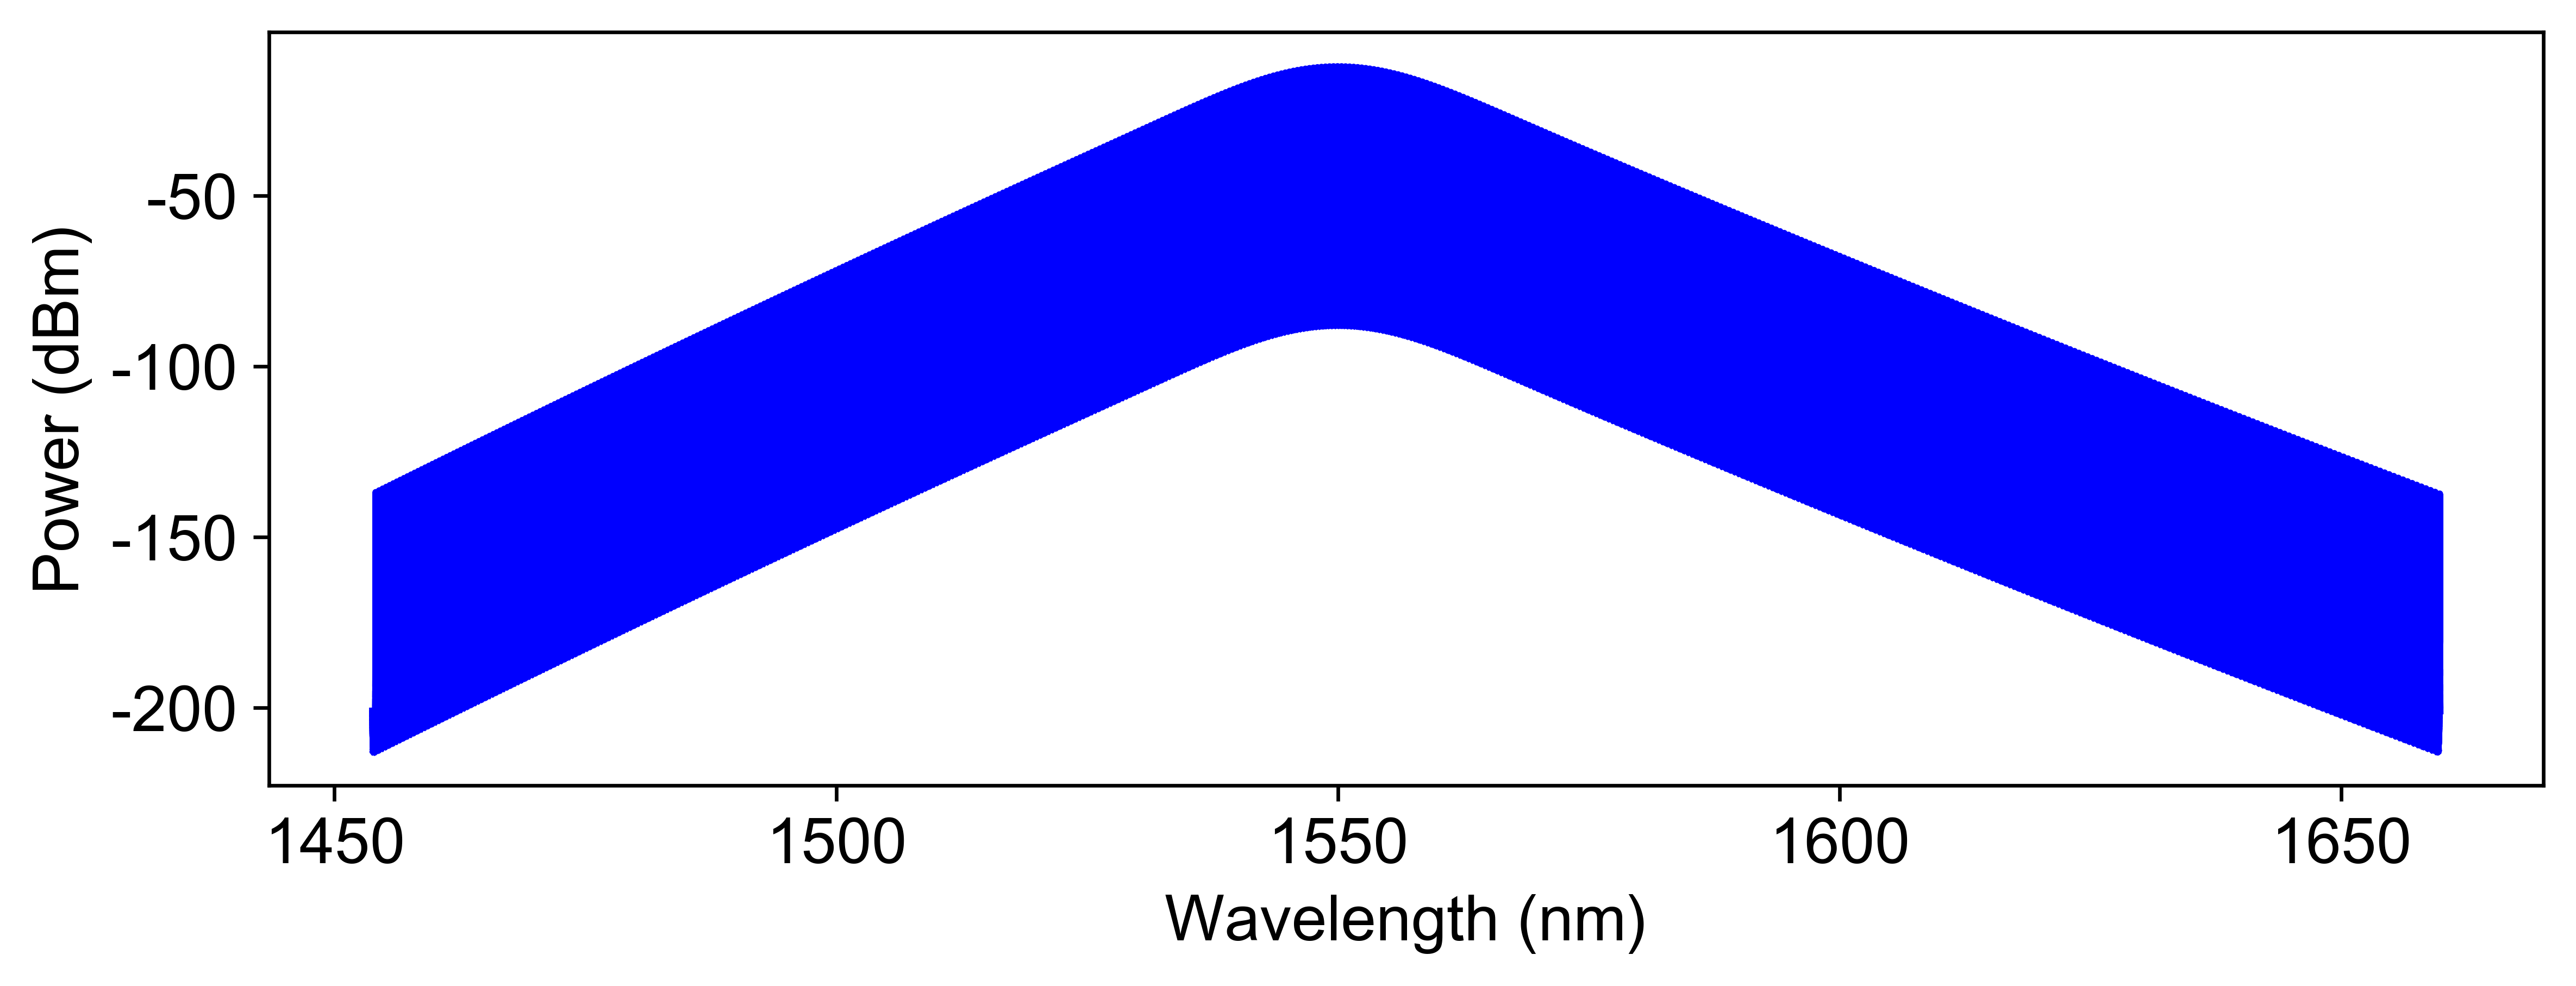
\includegraphics[width=0.48\linewidth]{figure/fig_23_0.png}
    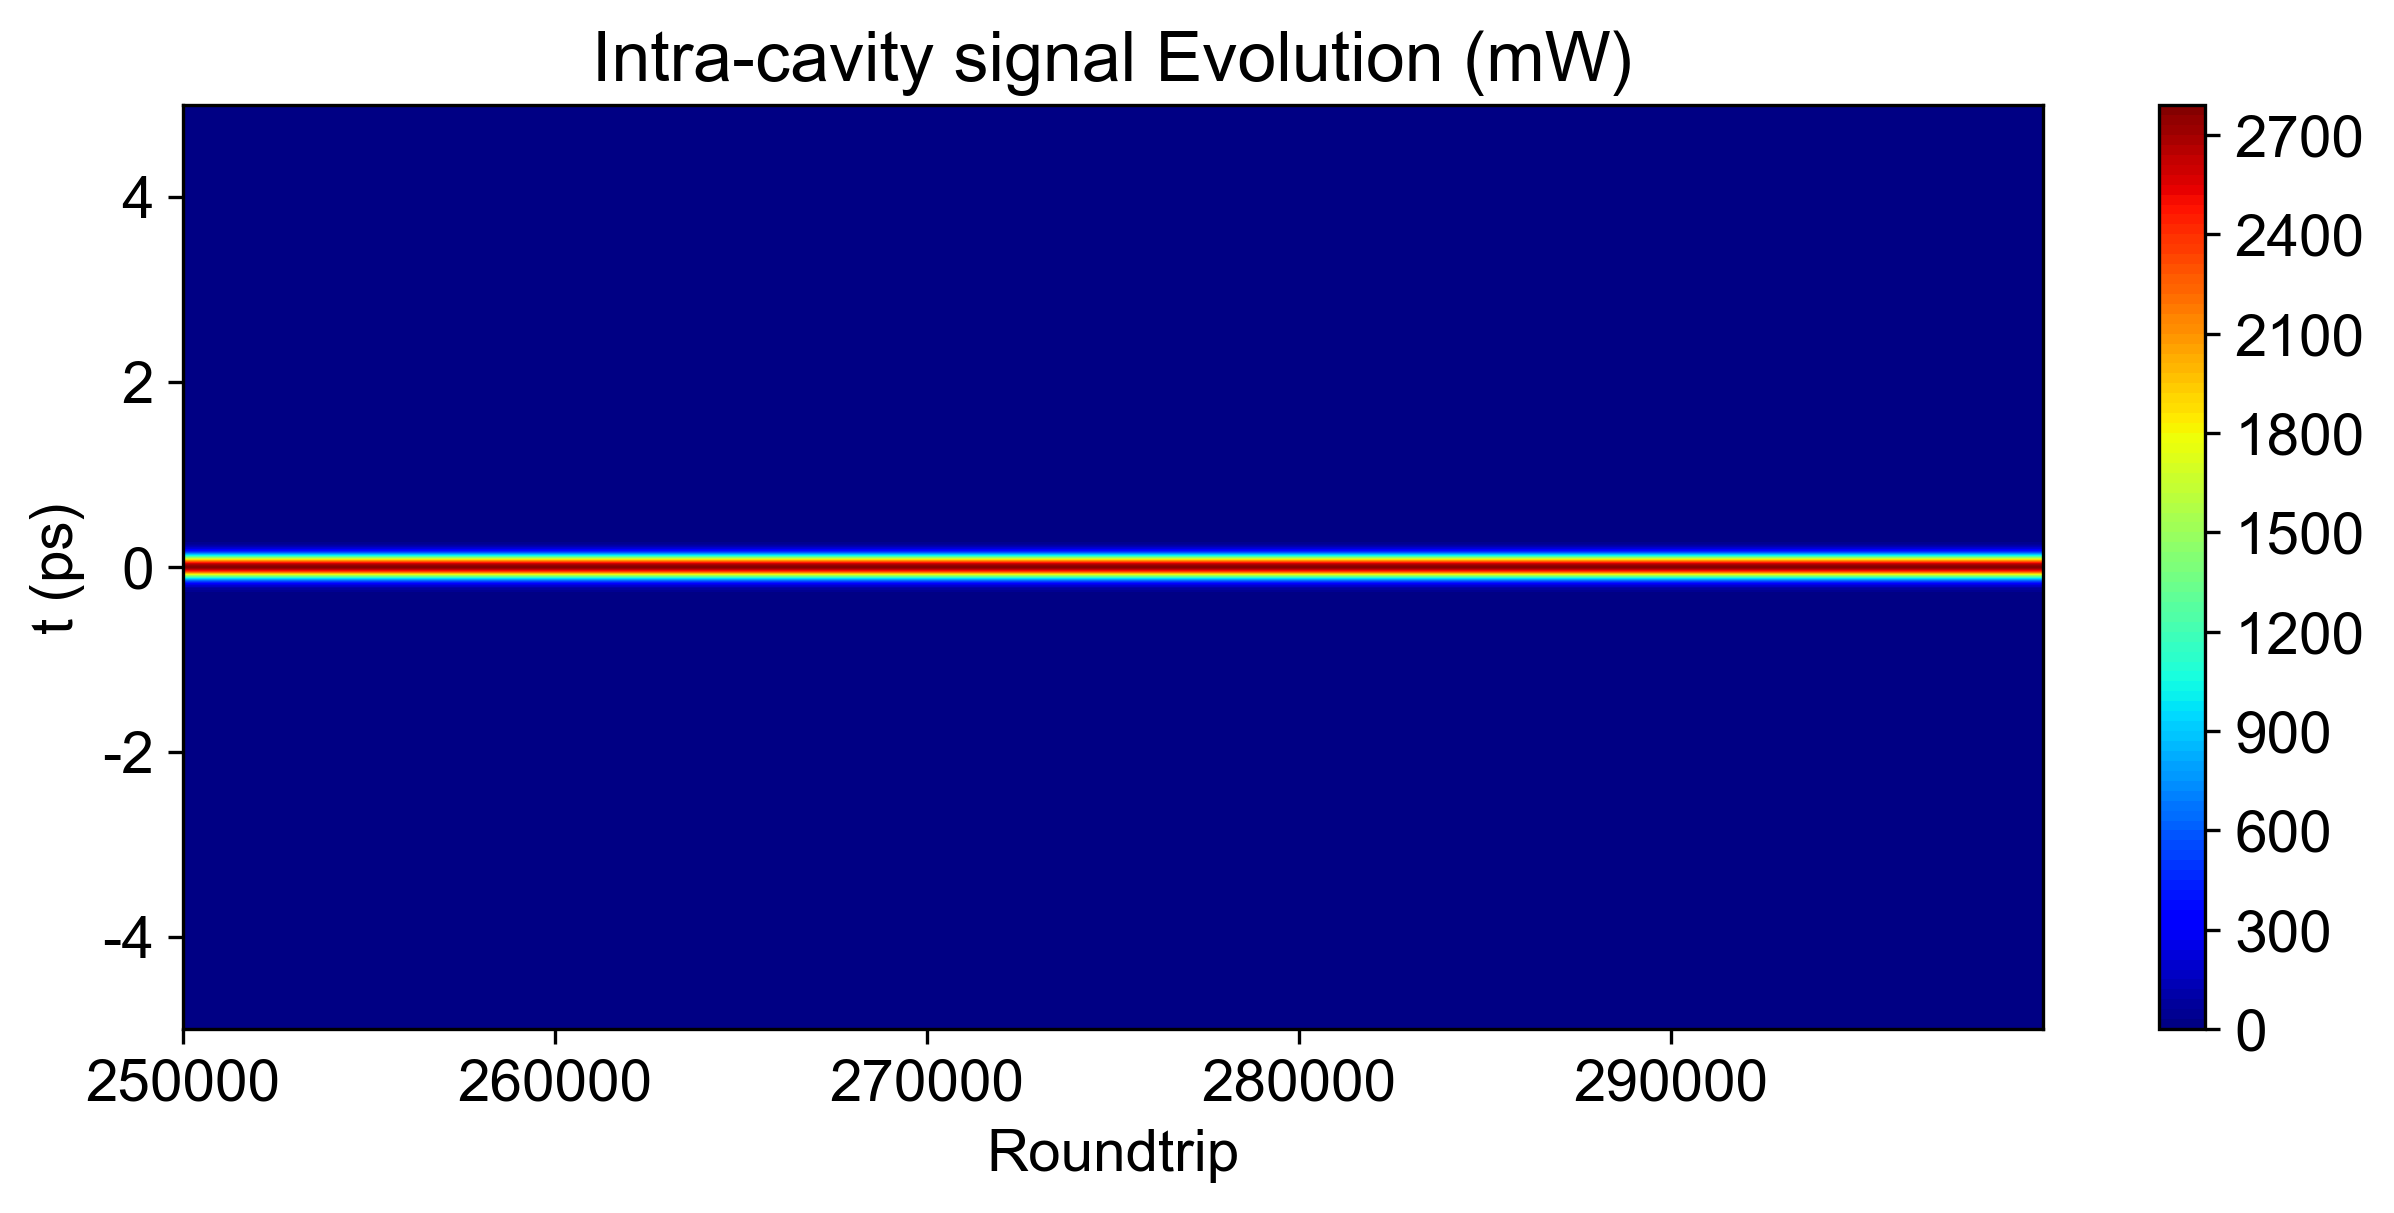
\includegraphics[width=0.48\linewidth]{figure/fig_24.png}
    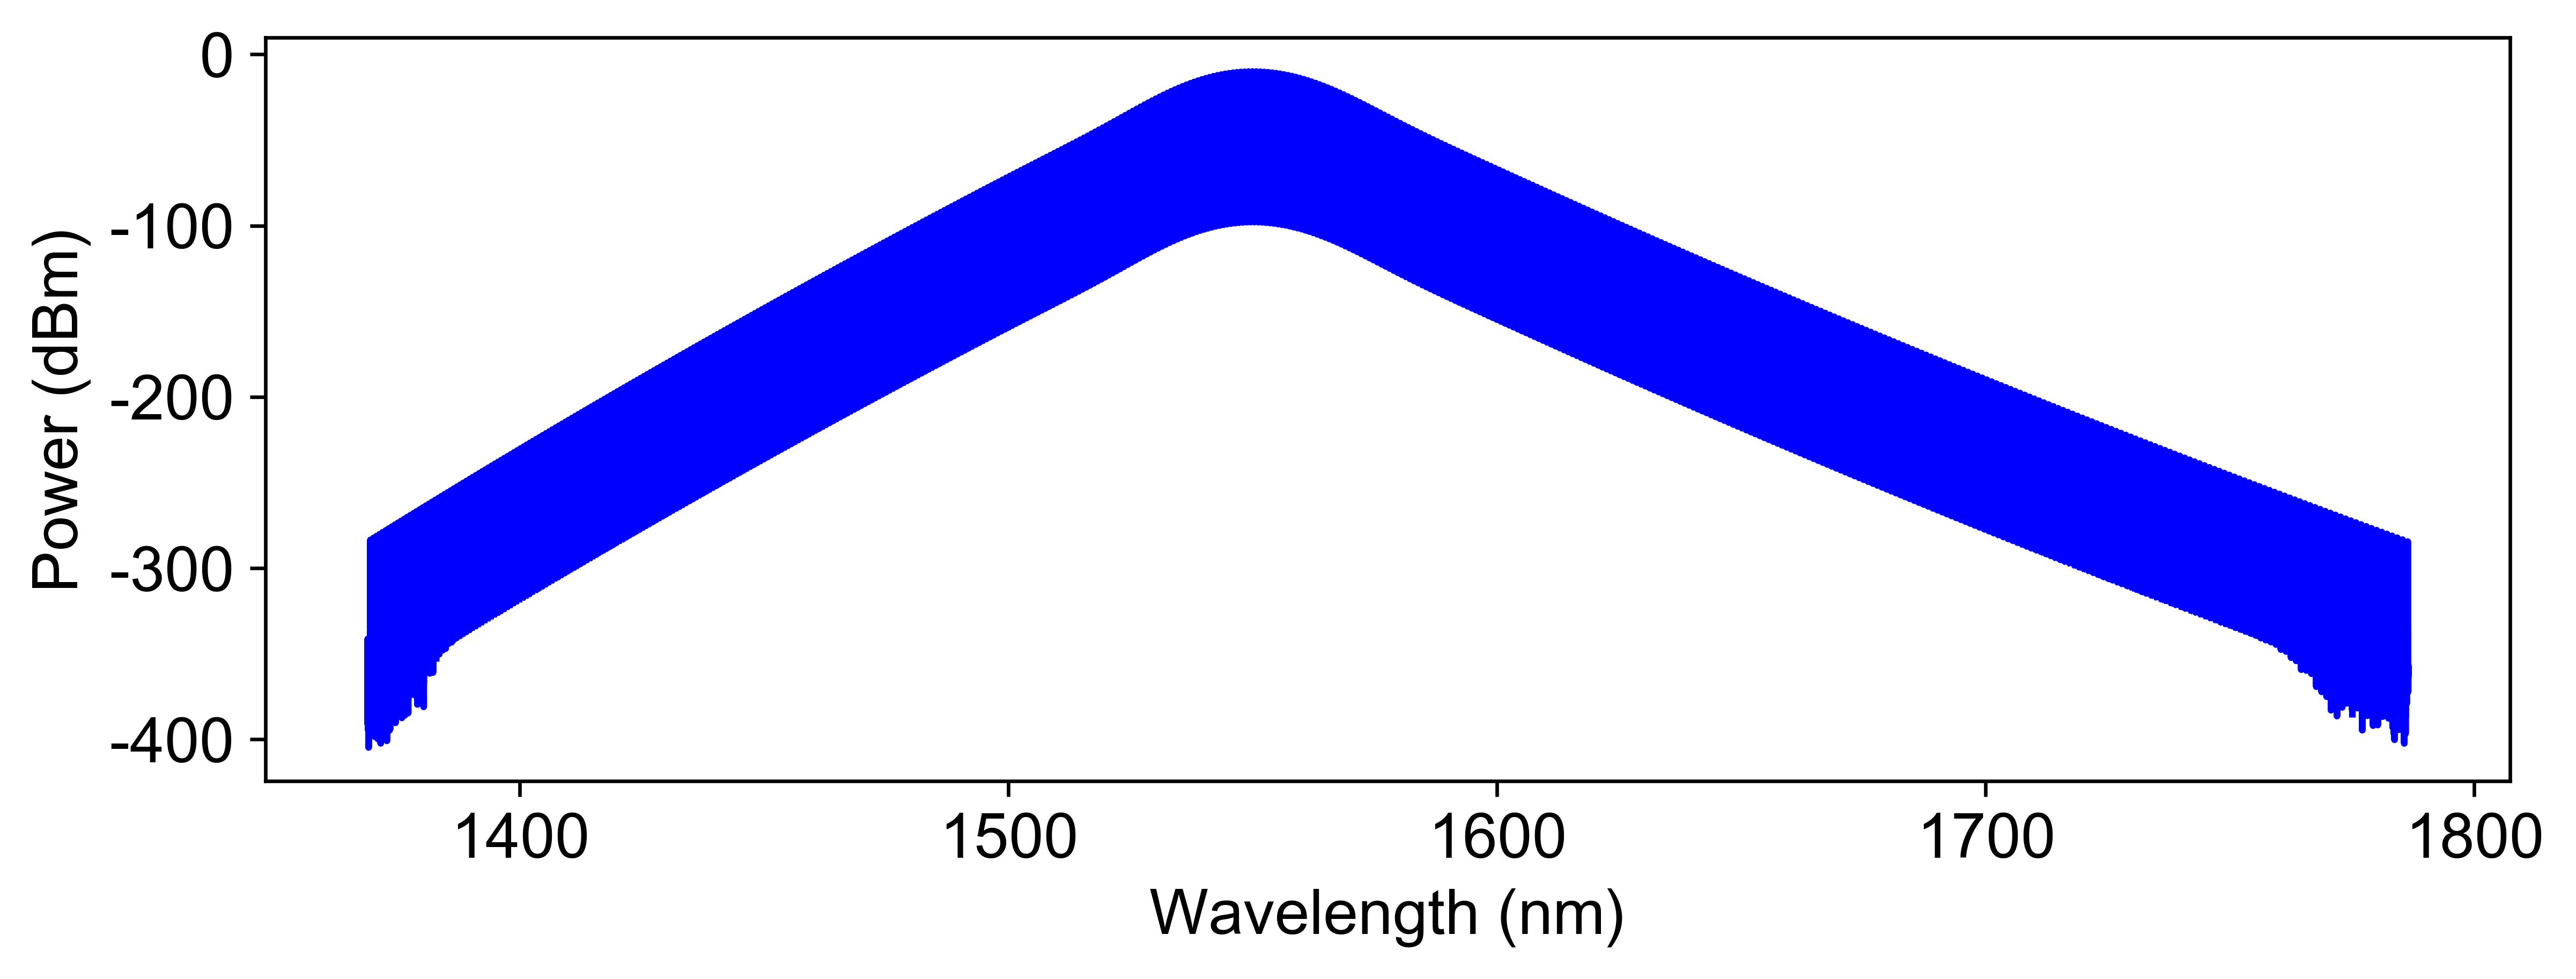
\includegraphics[width=0.48\linewidth]{figure/fig_24_0.png}
    \caption{左列:腔内信号光场的稳态,对应的光谱。从上到下$FSR$依次为:10,25,50,100GHz。}
    \label{fig:enter-label}
\end{figure}
$FSR$越大,越接近锁模态。
\section{泵浦转化效率}
% 只有在锁模的基础上讨论泵浦转化效率才有意义。\\
\begin{figure}[htbp]
    \centering
    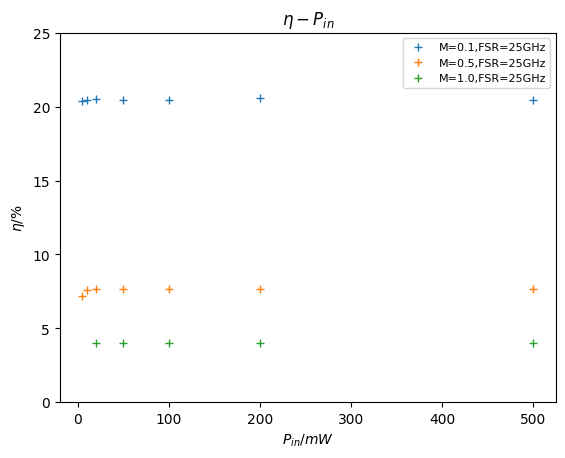
\includegraphics[width=0.99\linewidth]{figure/fig_25.png}
    \caption{不同调制深度下,泵浦转化效率和泵浦功率的关系图}
    \label{fig:enter-label}
\end{figure}
调制深度越大,泵浦光的耦合效率越低,因此转换效率越低。\\
泵浦功率变化时,增益介质的效率在饱和前都近似不变,锁模系统是线性的,不会饱和,因此转换效率近乎不变。\\
\section{本章小节}
调制深度,泵浦光功率,重频是影响锁模效果和泵浦转化效率的关键参数。本章通过数值仿真揭示了其定性关系。调制深度越大,锁模效果越好,但泵浦转化效率降低。重复频率越大,锁模效果越好,但泵浦转化效率降低。泵浦光功率越大,锁模效果越差,泵浦转化效率几乎不变,即输出功率正比于泵浦光功率。\\
本研究的目的是制造出重频在微波范围内、高转化效率、高功率的锁模激光器,但由于各参数的制约,三个条件不能同时满足。
